\documentclass[11pt,a4paper]{article}
% ============================================================
%  Shared preamble for the Medical Signal and Image Processing
%  Lab reports (English edition).  Compile with pdfLaTeX.
% ============================================================
\usepackage[T1]{fontenc}
\usepackage[utf8]{inputenc}
\usepackage{mathpazo}                     % Palatino text and math
\usepackage[scaled=0.92]{helvet}          % sans-serif for headings
\usepackage{courier}                      % monospace for code
\usepackage{amsmath,amssymb,bm}
\usepackage{microtype}
\usepackage[a4paper,left=2.4cm,right=2.4cm,top=2.9cm,bottom=2.5cm,headheight=22pt]{geometry}
\usepackage{xcolor}
\usepackage{graphicx}
\usepackage{float}
\usepackage{placeins}
\usepackage{booktabs,array,multirow,tabularx,longtable}
\usepackage{enumitem}
\usepackage{siunitx}
\usepackage{caption,subcaption}
\usepackage{fancyhdr}
\usepackage{titlesec}
\usepackage{listings}
\usepackage[most]{tcolorbox}
\usepackage{tikz}
\usepackage[colorlinks=true,linkcolor=primary,citecolor=primary,urlcolor=primary]{hyperref}

\linespread{1.06}
\setlength{\parindent}{0pt}
\setlength{\parskip}{0.55em}
\emergencystretch=3em

% ---------- colours ----------
\definecolor{primary}{HTML}{1B6B87}
\definecolor{accent}{HTML}{C2522B}
\definecolor{soft}{HTML}{EAF3F6}
\definecolor{ink}{HTML}{22313A}
\definecolor{muted}{HTML}{6B7A83}

% ---------- headings ----------
\titleformat{\section}
  {\sffamily\bfseries\LARGE\color{primary}}{\thesection}{0.7em}{}
  [{\vspace{-0.2em}\color{primary!35}\titlerule[0.8pt]}]
\titleformat{\subsection}
  {\sffamily\bfseries\large\color{ink}}{\thesubsection}{0.6em}{}
\titleformat{\subsubsection}
  {\sffamily\bfseries\normalsize\color{primary}}{\thesubsubsection}{0.5em}{}
\titlespacing*{\section}{0pt}{1.6em}{0.9em}
\titlespacing*{\subsection}{0pt}{1.3em}{0.5em}
\titlespacing*{\subsubsection}{0pt}{1.0em}{0.3em}

% ---------- header / footer ----------
\pagestyle{fancy}
\fancyhf{}
\renewcommand{\headrulewidth}{0.4pt}
\renewcommand{\headrule}{\hbox to\headwidth{\color{primary!45}\leaders\hrule height \headrulewidth\hfill}}
\fancyhead[L]{\sffamily\small\color{muted}Medical Signal and Image Processing Lab}
\fancyhead[R]{\sffamily\small\color{muted}\reportshorttitle}
\fancyfoot[C]{\sffamily\small\color{muted}\thepage}
\fancypagestyle{plain}{\fancyhf{}\fancyfoot[C]{\sffamily\small\color{muted}\thepage}\renewcommand{\headrulewidth}{0pt}}

% ---------- captions ----------
\captionsetup{font={small,sf},labelfont={bf,color=primary},labelsep=period,
  format=plain,justification=centering,skip=6pt}
\captionsetup[table]{position=above,skip=5pt}
\renewcommand{\arraystretch}{1.18}

% ---------- code listings ----------
\lstdefinestyle{code}{
  basicstyle=\ttfamily\footnotesize,
  keywordstyle=\color{primary}\bfseries,
  commentstyle=\color{muted}\itshape,
  stringstyle=\color{accent},
  backgroundcolor=\color{soft},
  frame=single, rulecolor=\color{primary!30},
  framerule=0.5pt, xleftmargin=0pt, framexleftmargin=4pt,
  aboveskip=0.8em, belowskip=0.6em, breaklines=true,
  showstringspaces=false, columns=fullflexible, keepspaces=true,
  upquote=true, tabsize=2}
\lstset{style=code}

% ---------- boxes ----------
\newtcolorbox{keyresult}[1][]{enhanced,breakable,
  colback=soft,colframe=primary,boxrule=0pt,
  borderline west={3pt}{0pt}{primary},
  arc=2pt,left=10pt,right=10pt,top=7pt,bottom=7pt,
  fonttitle=\sffamily\bfseries,coltitle=primary,
  attach boxed title to top left={yshift=-2mm,xshift=0mm},
  boxed title style={colback=white,boxrule=0pt,top=0pt,bottom=0pt,left=0pt},
  #1}
\newtcolorbox{notebox}[1][]{enhanced,breakable,
  colback=white,colframe=accent!70,boxrule=0pt,
  borderline west={3pt}{0pt}{accent},
  arc=2pt,left=10pt,right=10pt,top=6pt,bottom=6pt,#1}
\newtcolorbox{taskbox}[1][Task]{enhanced,breakable,
  colback=black!4,colframe=black!4,boxrule=0pt,
  borderline west={2.5pt}{0pt}{muted},
  arc=1pt,left=9pt,right=9pt,top=5pt,bottom=5pt,
  fontupper=\small,
  title={\sffamily\bfseries\scriptsize\textcolor{muted}{\MakeUppercase{#1}}},
  coltitle=muted,fonttitle=\sffamily\bfseries\scriptsize,
  attach title to upper={\par\smallskip}}
\newcommand{\pending}[1]{%
  \begin{tcolorbox}[enhanced,colback=white,colframe=white,boxrule=0pt,
    borderline={0.6pt}{0pt}{muted,dashed},arc=2pt,left=8pt,right=8pt,top=5pt,bottom=5pt]
    \sffamily\small\color{muted}Translation pending: #1
  \end{tcolorbox}}

% ---------- question / answer helpers ----------
\newcommand{\question}[2]{%
  \subsection*{\textcolor{accent}{Q#1}\texorpdfstring{\hspace{0.6em}}{ }#2}%
  \addcontentsline{toc}{subsection}{Q#1\texorpdfstring{\quad}{ }#2}}
\newcommand{\answer}{\textbf{\textsf{\textcolor{primary}{Answer.}}}\ }

% ---------- convenient units / symbols ----------
\newcommand{\mV}{\si{\milli\volt}}
\newcommand{\Hz}{\si{\hertz}}

% ---------- title page ----------
% needs: \reportnumber \reporttitle \reportsubtitle
%        \authorone \authortwo \instructor \semester  (authors.tex)
\newcommand{\makereporttitle}{%
  \begingroup
    \thispagestyle{empty}
    \centering
    \vspace*{1.2cm}
    
\includegraphics[width=3.2cm]{sharif-logo.png}\par\vspace{0.9cm}
    {\sffamily\bfseries\Large\color{ink}Sharif University of Technology\par}
    \vspace{0.3cm}
    {\sffamily\large\color{muted}Medical Signal and Image Processing Lab\par}
    \vspace{1.0cm}
    {\color{primary}\rule{0.55\textwidth}{1.2pt}\par}
    \vspace{1.0cm}
    {\sffamily\small\color{accent}\textls[150]{\MakeUppercase{\reportnumber}}\par}
    \vspace{0.5cm}
    {\sffamily\bfseries\fontsize{26}{31}\selectfont\color{primary}\reporttitle\par}
    \vspace{0.6cm}
    {\sffamily\large\color{ink}\reportsubtitle\par}
    \vspace{1.0cm}
    {\color{primary}\rule{0.55\textwidth}{1.2pt}\par}
    \vspace{1.6cm}
    {\sffamily\bfseries\color{muted}\small\textls[100]{PREPARED BY}\par}
    \vspace{0.4cm}
    {\sffamily\Large\color{ink}\authorone\par}
    \vspace{0.2cm}
    {\sffamily\Large\color{ink}\authortwo\par}
    \vspace{1.3cm}
    {\sffamily\color{muted}Instructor:\ \textbf{\color{ink}\instructor}\par}
    \vfill
    {\sffamily\color{muted}\semester\par}
    \vspace{0.8cm}
    \clearpage
  \endgroup}
% inline reference markers such as [1, 2] (the reference list is added in the final part)
\newcommand{\rc}[1]{[#1]}

% Author and course metadata (shared by all reports).
\newcommand{\authorone}{Mohammad Reza Mahdavi}
\newcommand{\authortwo}{Reza Kazemeini Moghaddam}
\newcommand{\instructor}{Marzieh Barakat}
\newcommand{\semester}{Fall Semester 2026}


\newcommand{\reportnumber}{Experiment 1}
\newcommand{\reporttitle}{Display and Analysis of Biosignals}
\newcommand{\reportsubtitle}{Sampling, Fourier Transform and Time--Frequency Analysis of EEG, ECG, EOG and EMG}
\newcommand{\reportshorttitle}{Biosignal Time--Frequency Analysis}

\graphicspath{{figures/}}
\hypersetup{pdftitle={Experiment 1: Display and Analysis of Biosignals},pdfauthor={\authorone, \authortwo}}

\begin{document}
\makereporttitle
\tableofcontents
\clearpage

\section{Objective and Analysis Method}

The aim of this experiment is to examine the relation between the temporal shape of vital signals and their frequency content, and how this content changes over time. With real data, we examine the brain signal before and during seizure activity, the cardiac signal with different kinds of beats, eye movements, and healthy and diseased muscle activity. For each part, we interpret the time-domain display, the Fourier transform and the spectrogram together, because a single overall spectrum does not specify when events occur.

\subsection{Data and Physical Axes}

The data were read from the four files that accompany the exercise statement. For all signals, the time axis was built from the number of samples and the sampling frequency. In time slicing, the beginning of an interval is included and its end is excluded; a five-second interval therefore contains exactly five times the sampling rate in samples. The original data of none of the parts were rewritten.

\begin{center}
\begin{tabular}{@{}lccc@{}}
\toprule
\textbf{Data} & \textbf{Sampling rate (Hz)} & \textbf{Channels} & \textbf{Duration (s)}\\
\midrule
EEG & 256  & 32 & 64\\
ECG & 360  & 2  & 1805.556\\
EOG & 128  & 2  & 60\\
EMG & 4000 & $1\times3$ & 12.715\ /\ 27.584\ /\ 36.965\\
\bottomrule
\end{tabular}
\end{center}

The EMG durations in the table are given in the order healthy, myopathy, neuropathy. The \texttt{TIME} vector in the ECG file has 720000 values, whereas the signal matrix has 650000 rows; this vector was therefore set aside and the correct time axis was reconstructed. For amplitudes that have no calibration factor in the exercise file, the recorded unit or a.u.\ (arbitrary units) is used. The general physiological amplitude range given in the course notes does not, on its own, determine the conversion factor of these files to volts.

\subsection{Fourier Transform and Power Spectral Density}

For a signal with $N$ samples, the frequency axis and the Fourier transform are defined as
\begin{equation}
X[k]=\sum_{n=0}^{N-1}x[n]\,e^{-j2\pi kn/N},\qquad
f_k=\frac{k f_s}{N},\qquad
t_n=\frac{n}{f_s}.
\label{eq:dft}
\end{equation}
The one-sided amplitude spectrum was built from the absolute value of the FFT divided by $N$. The amplitude of the interior points is doubled, but the DC and Nyquist points are not. The unit of this spectrum is the same as that of the signal amplitude. The power spectral density (PSD) is a different quantity, with units of squared amplitude per hertz. Welch's method reduces the fluctuation of the spectral estimate by averaging the spectra of overlapping windows. To compare the structure of the oscillations, the mean of each segment was removed before spectral analysis; the time-domain plots show the raw data.

\subsection{Time--Frequency Analysis}

\begin{equation}
\mathrm{STFT}(m,k)=\sum_{n}x[n]\,w[n-mH]\,e^{-j2\pi kn/N_{\mathrm{FFT}}},\qquad
H=L-N_{\mathrm{overlap}}.
\label{eq:stft}
\end{equation}
The spectrogram is drawn from the power of the short-time transform. A longer window improves the frequency resolution and weakens the time localization. Zero-padding only makes the frequency display grid finer; it does not create new information or any real additional resolution. To compare spectrograms, the same color scale is used within each set.

\section{Part 1: Brain Signal (EEG)}

\begin{taskbox}[Part 1: introduction in the lab manual]
A segment of EEG is provided in the file \texttt{sig\_EEG.mat}. The file contains a matrix \texttt{Z}, a 32-channel signal over time samples. The sampling frequency and the channel labels (in channel order) are stored in the variable \texttt{des}. The signal belongs to an epileptic patient and was recorded before and during a seizure. Since the signal is real, muscle artifacts are clearly visible in it.
\end{taskbox}

\subsection{Question 1: Displaying Channel 5}
\begin{taskbox}
Plot the signal of the 5th channel in the time domain. Set the time axis so that it is displayed in seconds. Set the figure height and width manually so that the changes of the signal shape over time are clearly visible. Write the channel label as the y-axis label or the figure title.
\end{taskbox}

According to the data labels, channel 5 is C3; this name refers to the left central region of the hemisphere in the electrode naming scheme. Figure~\ref{fig:c3full} shows the complete 64-second recording with the time axis in seconds. The differences in waveform shape across the recording, and the growth of amplitude in the later parts, can be seen. The last sample lies at 63.9961 seconds, and the recording length follows from the number of samples divided by the sampling rate.

\begin{figure}[H]
\centering
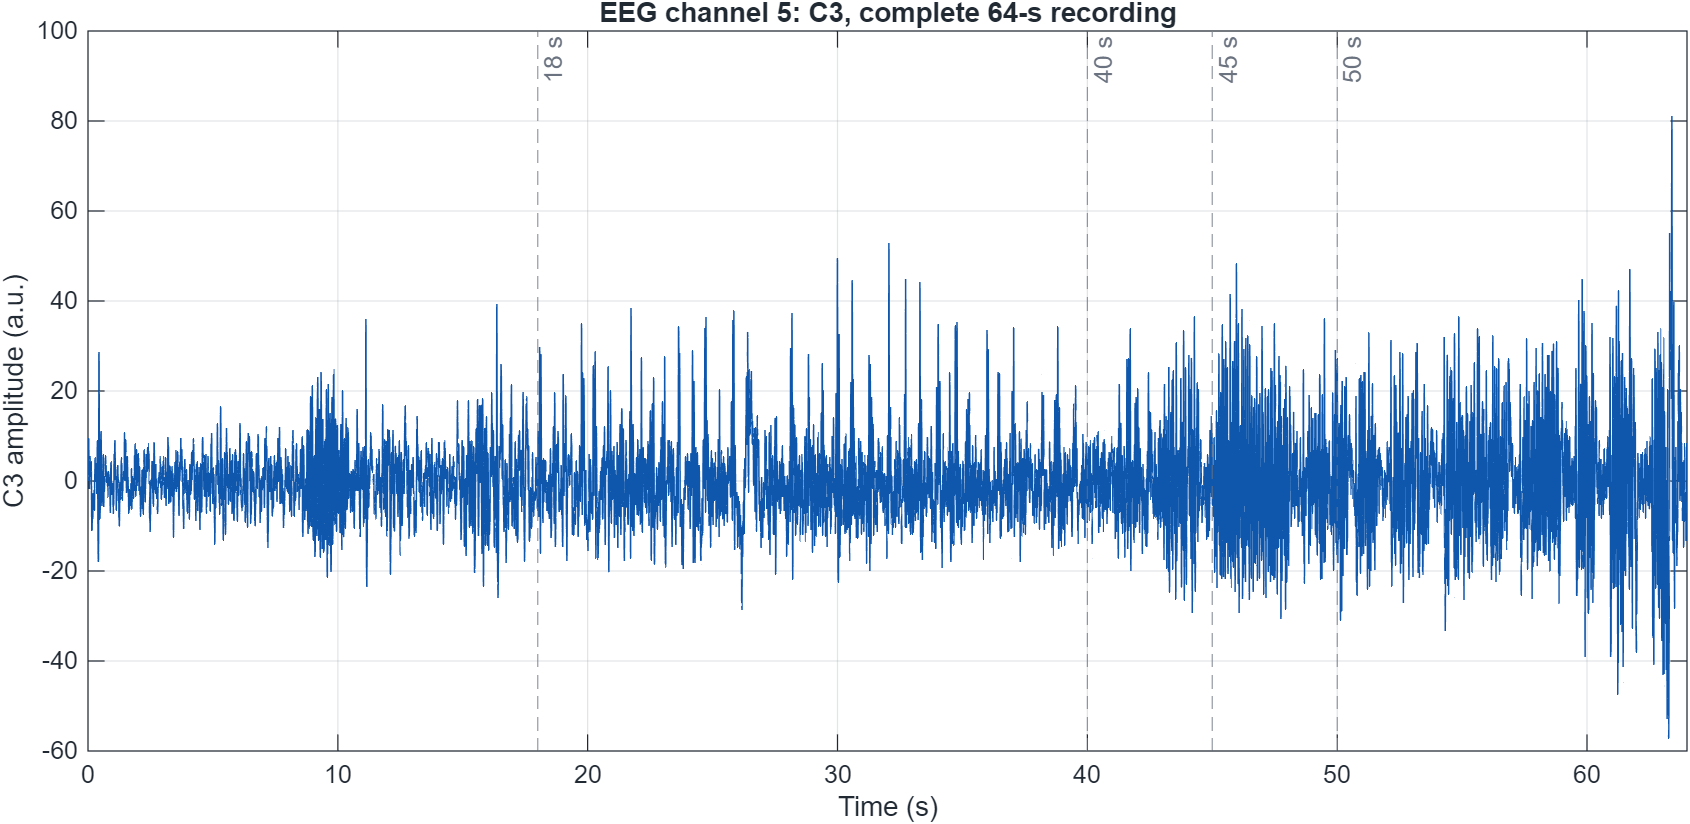
\includegraphics[width=\textwidth]{fig01_c3_full_recording.png}
\caption{Time display of the complete channel 5 (C3) and approximate boundaries for the morphology examination.}
\label{fig:c3full}
\end{figure}

\paragraph{Time--frequency spectrogram of the whole C3 signal.} To complete the time display, Figure~\ref{fig:c3stft} shows the distribution of power density over the entire 64-second recording. A two-second Hamming window with a 0.25~s step was used, and the mean of each window was removed. A warmer color indicates a greater power density; the color value is in dB relative to $1\ \mathrm{a.u.}^2/\mathrm{Hz}$ and is not the direct amplitude of the wave. For example, 10~dB corresponds to $10\ \mathrm{a.u.}^2/\mathrm{Hz}$.

\begin{figure}[H]
\centering
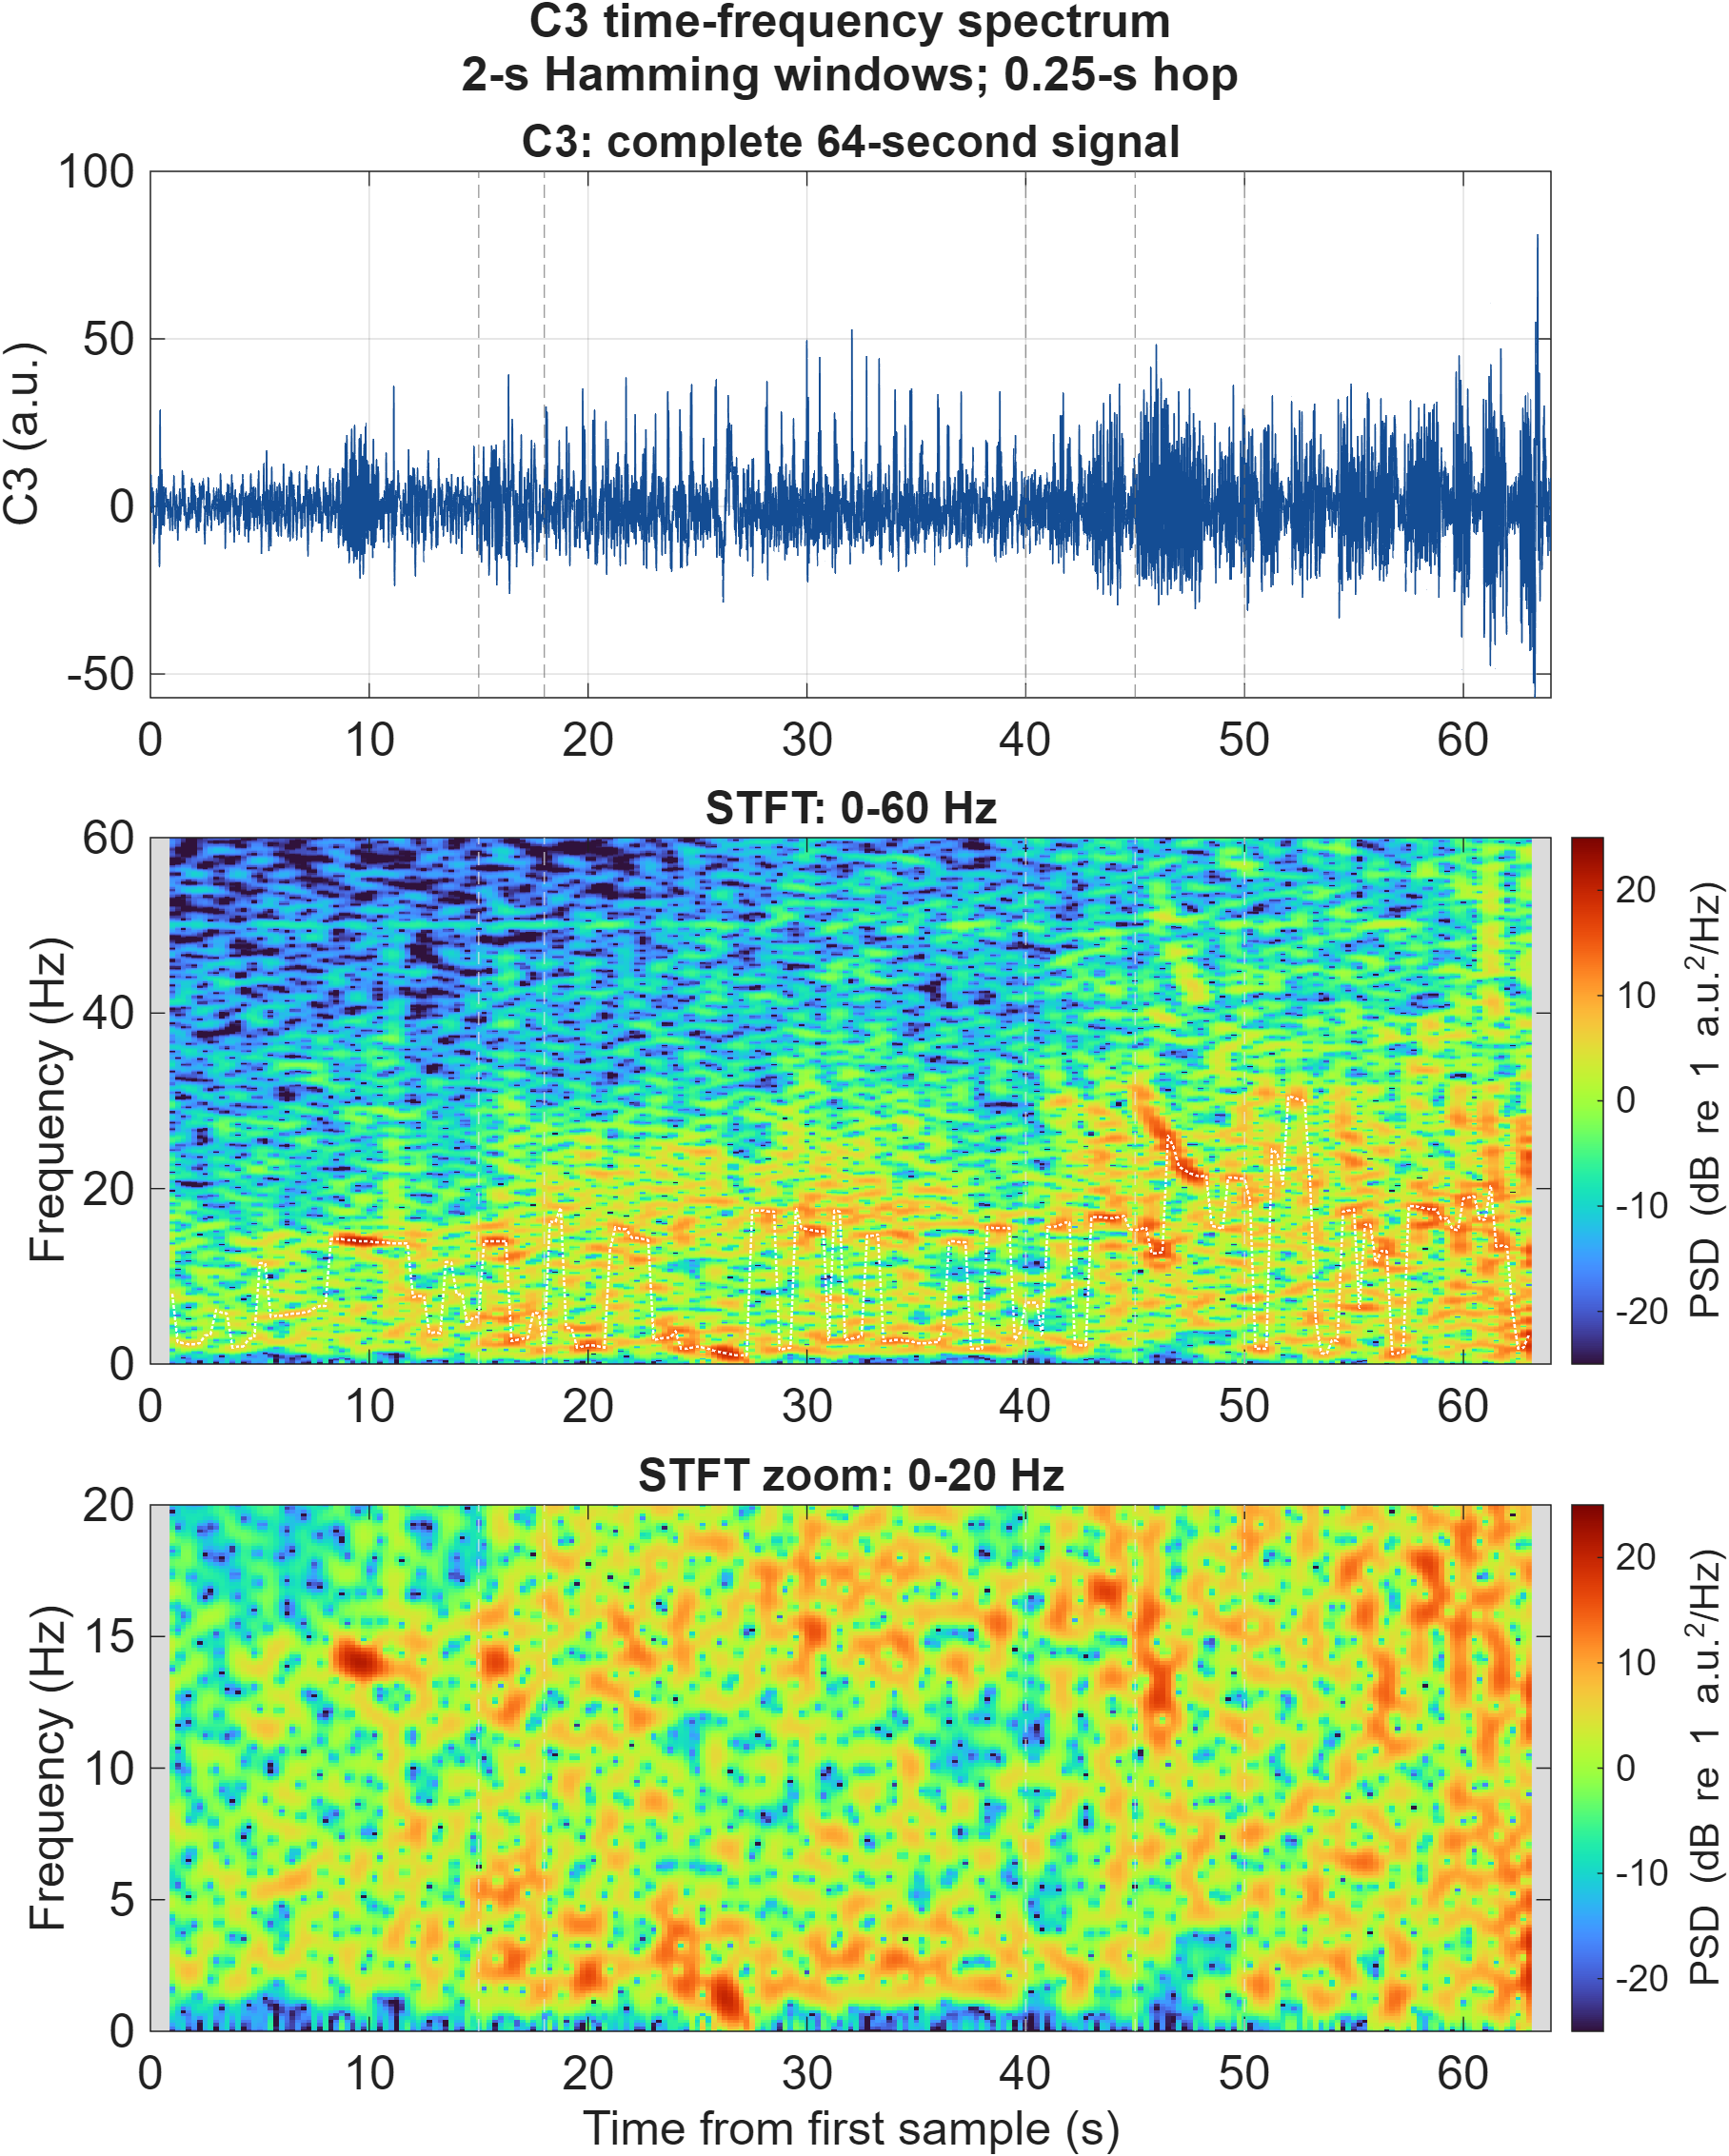
\includegraphics[width=0.82\textwidth]{fig02_c3_stft_full_recording.png}
\caption{Waveform and spectrogram of the whole C3 channel over 0--60~Hz and 0--20~Hz with the same color scale; the white line marks the strongest peak of each window, only within 1--40~Hz.}
\label{fig:c3stft}
\end{figure}

The times are window centers; the gray margins do not have a complete window. The spacing of the FFT grid is 0.125~Hz, but this value comes from zero-padding, and the true resolution is limited by the window length; the equivalent noise bandwidth of the window is about 0.68~Hz. This display complements Question~1 and does not change the settings requested for Question~8.

\subsection{Question 2: Examining Waveform Changes}
\begin{taskbox}
Examine the temporal-morphological features of the signal at different times (the first 15 seconds, approximately 18 to 40 seconds, approximately 45 to 50 seconds, and the final part from 50 seconds to the end of the signal). What notable features are seen in the signal?
\end{taskbox}

In the first 15 seconds, the background oscillations have a lower amplitude. In the range of 18 to 40 seconds, sharp discharges with a relatively regular repetition are seen on top of the background activity. In 45 to 50 seconds, the oscillations are denser and faster. From 50 seconds onward, the waves become more irregular and contain slower components and larger transients. In Figure~\ref{fig:c3four} each interval is displayed separately; the vertical scale of each panel must be read, and the apparent height on the page is not an independent measure of amplitude.

\begin{center}
\begin{tabular}{@{}ccc@{}}
\toprule
\textbf{Interval (s)} & \textbf{Peak-to-peak amplitude} & \textbf{AC RMS}\\
\midrule
0--15  & 59.41  & 6.09\\
18--40 & 81.34  & 8.79\\
45--50 & 78.80  & 12.50\\
50--64 & 138.08 & 13.18\\
\bottomrule
\end{tabular}
\end{center}

The amplitude values in the table are in a.u. The increase of the RMS from about 6.09 at the beginning of the recording to 13.18 at its end is consistent with the growth of amplitude. Nevertheless, part of the fast variation may be due to muscle artifacts, and its exact share cannot be separated from a single channel.

\begin{figure}[H]
\centering
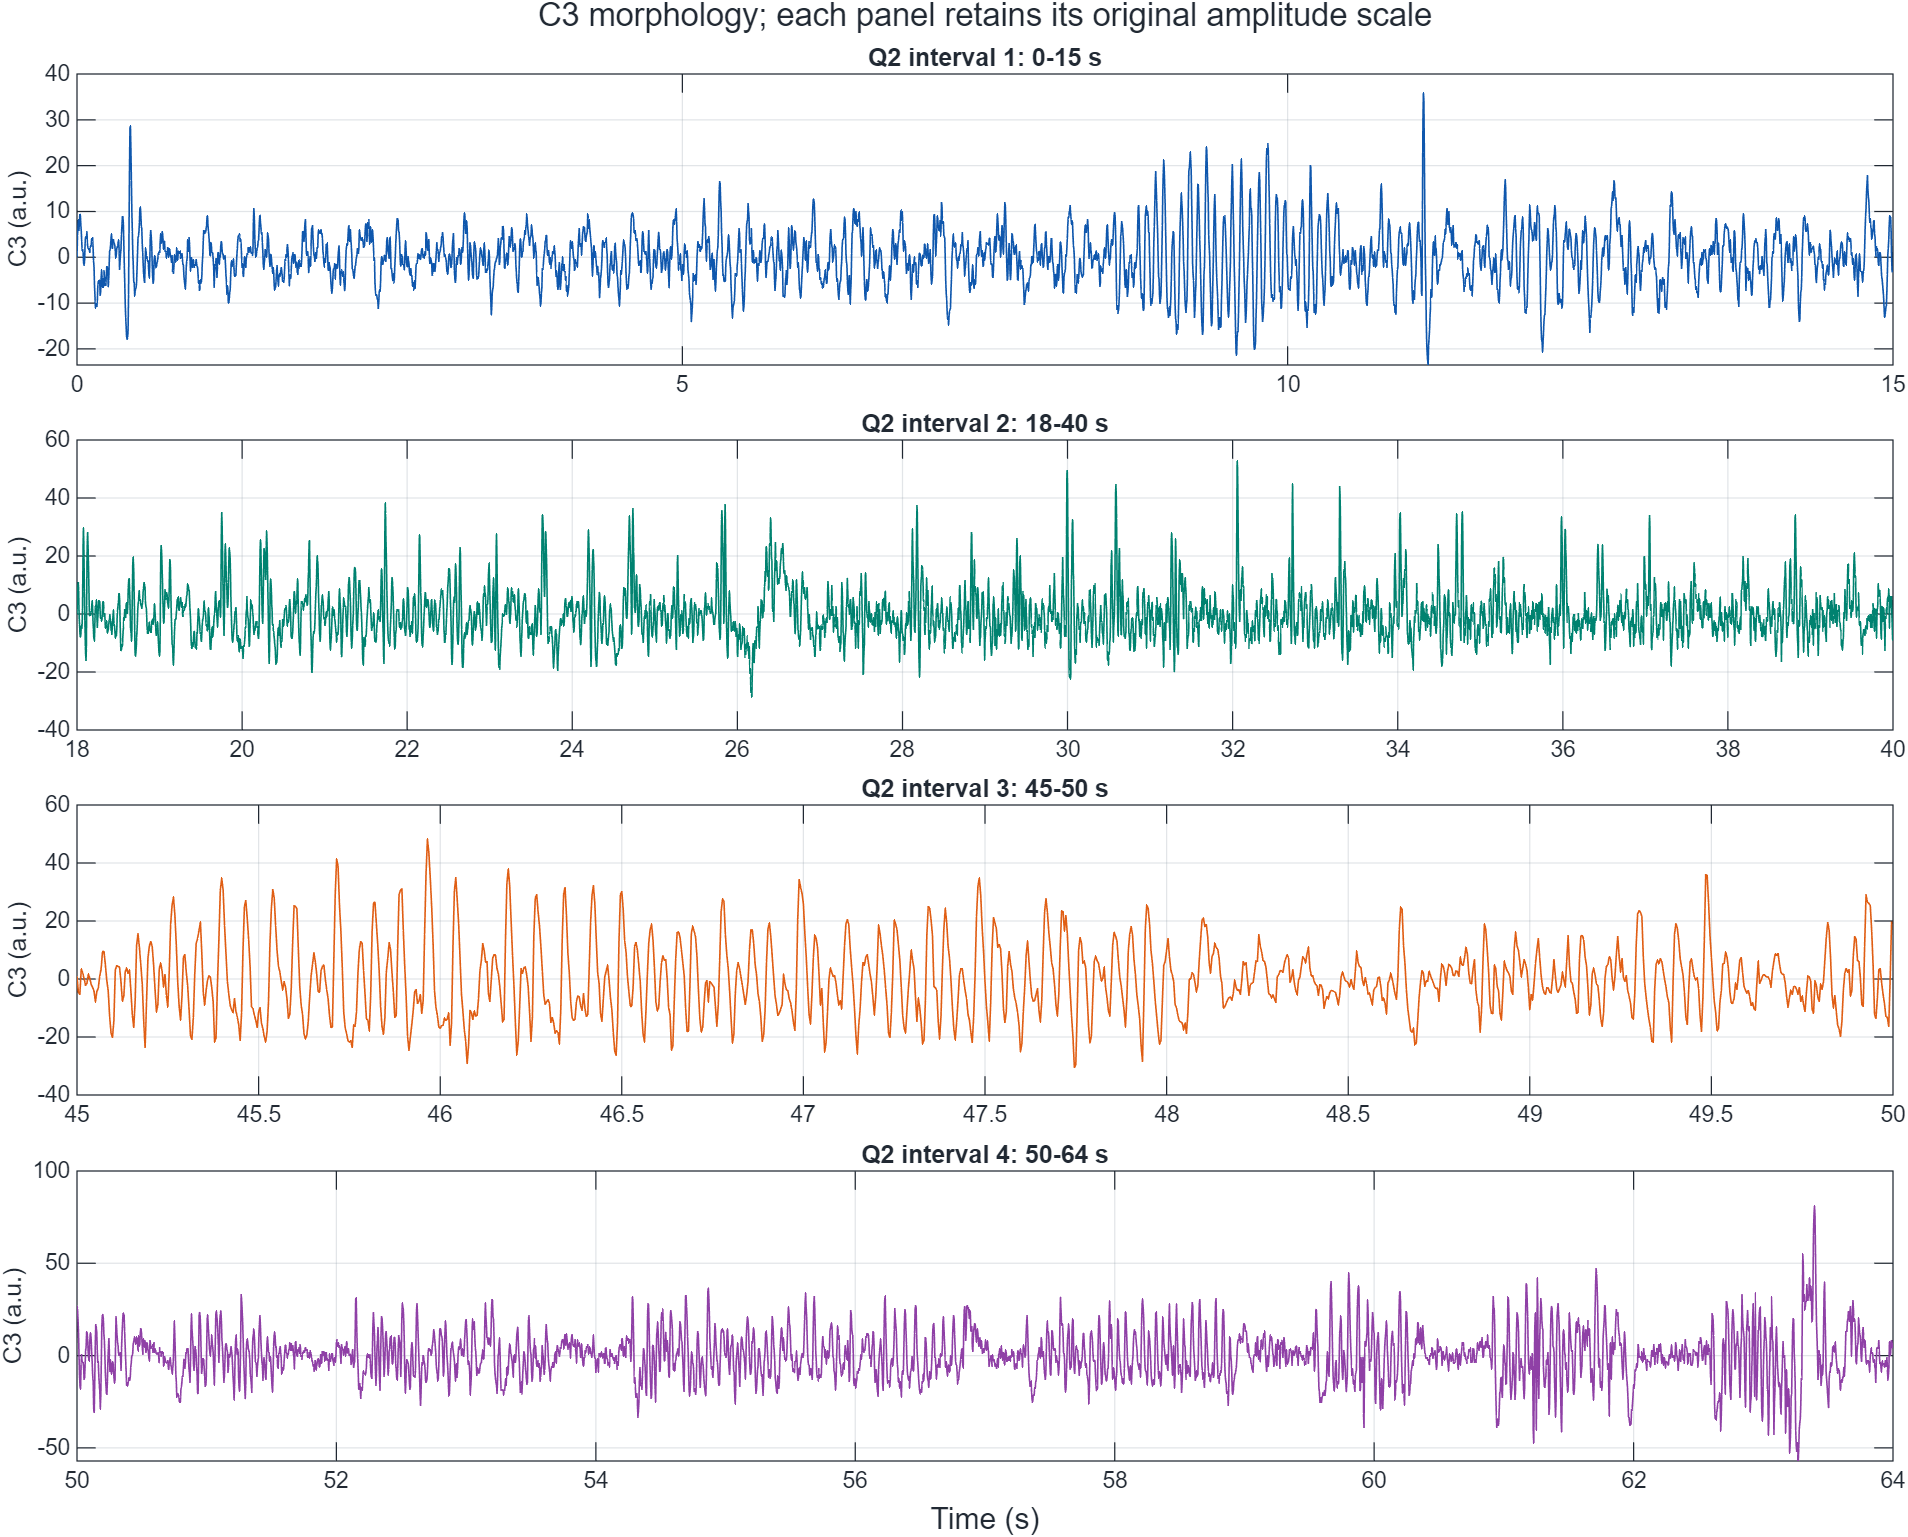
\includegraphics[width=\textwidth]{fig03_c3_four_intervals.png}
\caption{The four time intervals requested for examining the waveform shape of the brain channel.}
\label{fig:c3four}
\end{figure}

\subsection{Question 3: Comparison with Another Channel}
\begin{taskbox}
Plot another channel of your choice. Is the signal shape over time the same as in the 5th channel?
\end{taskbox}

Channel C4 was chosen for comparison with C3. The comparison of the two channels is shown in Figure~\ref{fig:c3c4}, and the display of all channels in Figure~\ref{fig:all32}.

\answer Overall, the signals of different channels share similarities in the general pattern of activity. For example, up to about second 27, and especially in the interval from 1 to 26 seconds, the general trend of variation is roughly similar. Nevertheless, the intensity, the time of occurrence and the clarity of the activities can differ from one channel to another, and some activities are not seen at the same level in all channels.

For instance, the relatively regular spikes present in channel C3 are seen in the other channels with the same regularity and prominence, or with a smaller amplitude. Also, the slower and more irregular envelopes seen in C3 from about second 40 onward do not appear in the same form in the other channels. By contrast, in the final part of the recording, high-power spikes are seen in different channels, which is one of the observable similarities among them.

\begin{figure}[H]
\centering
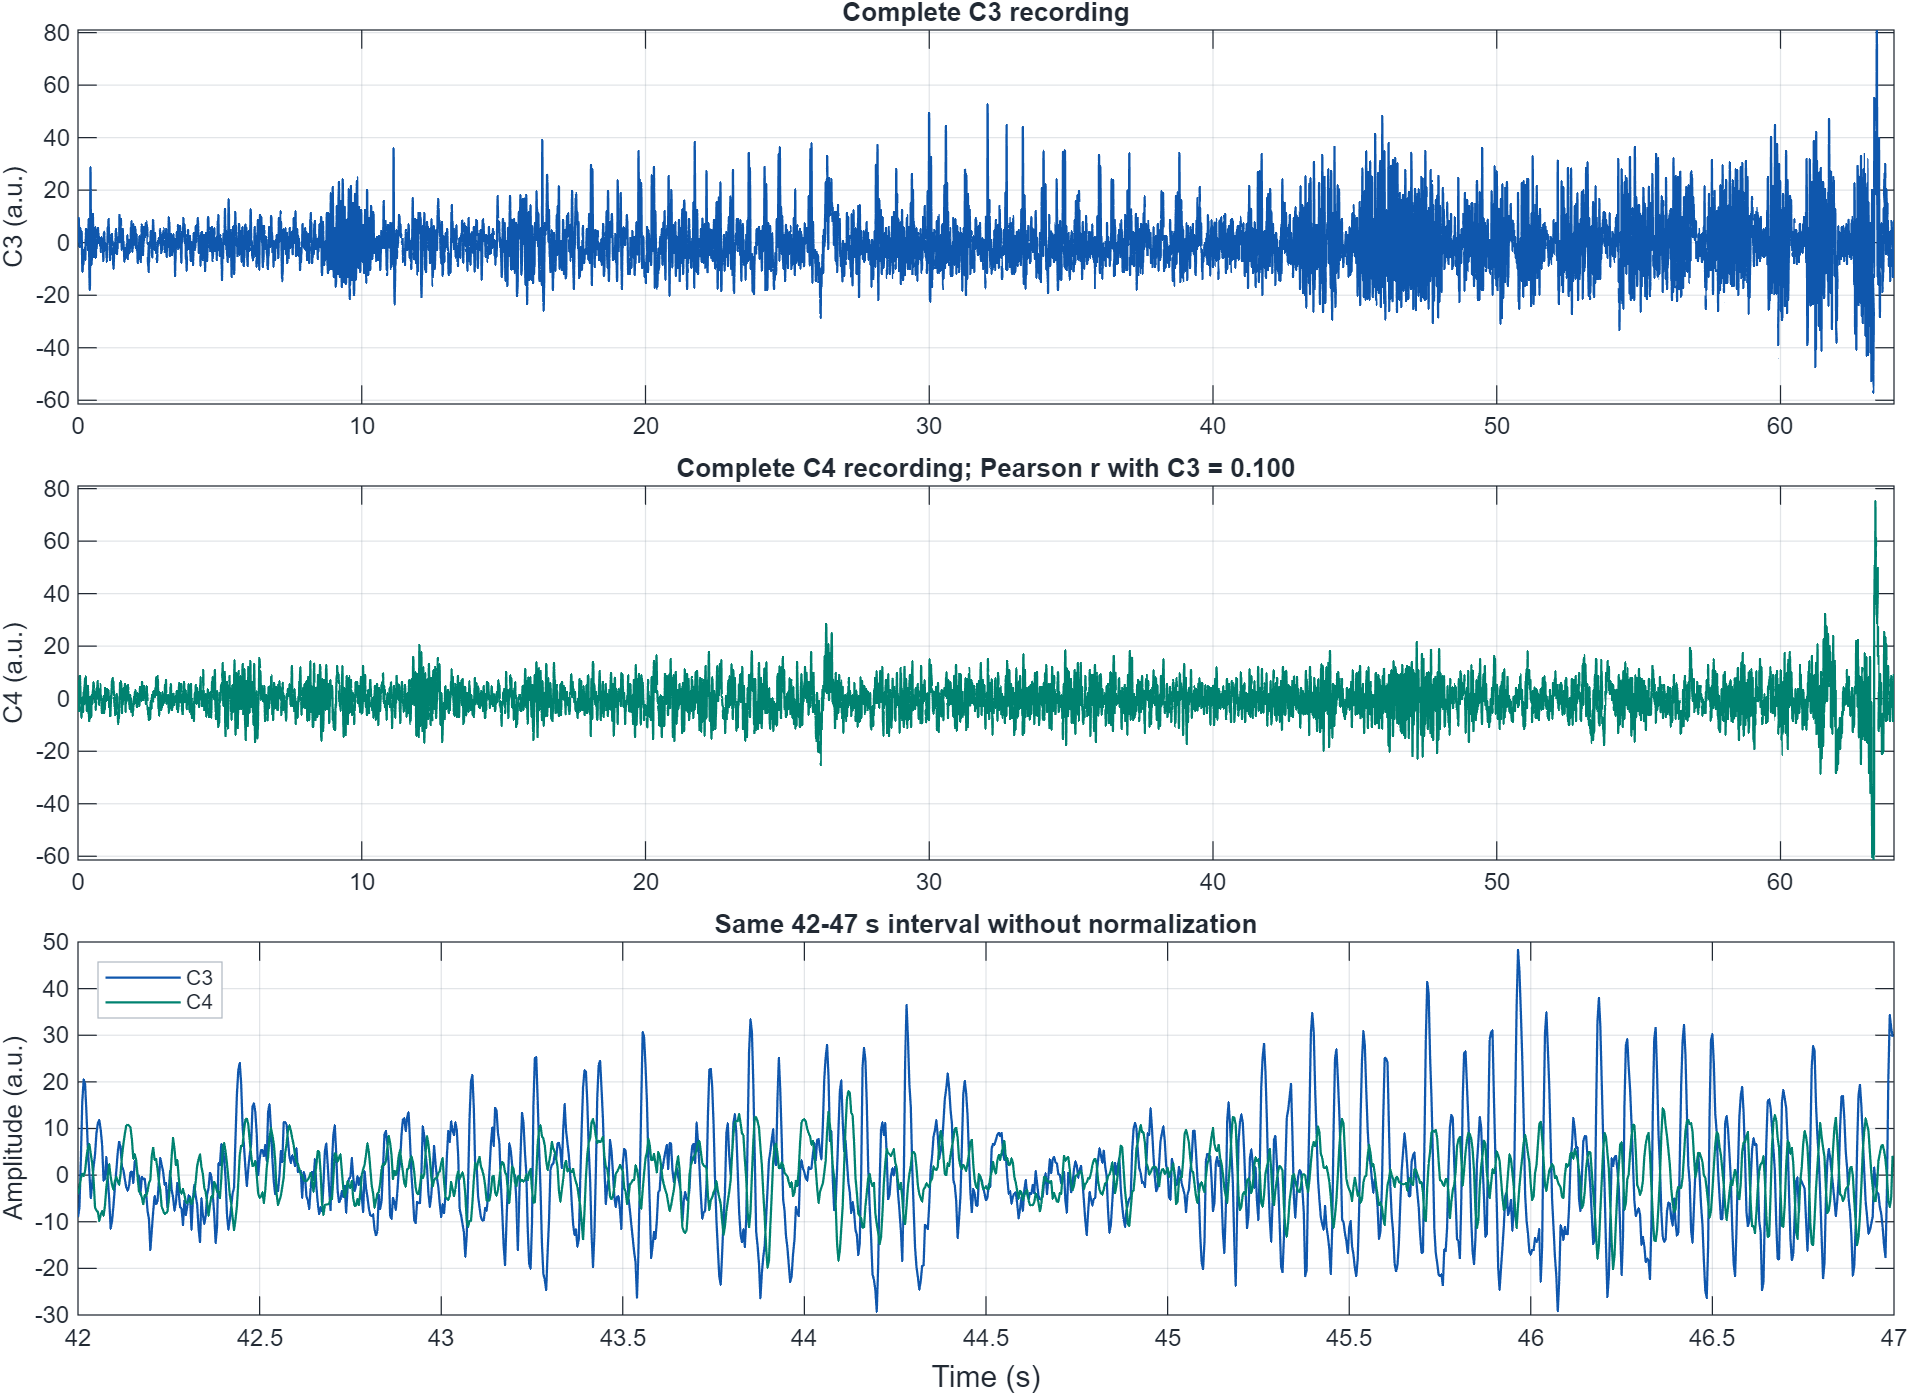
\includegraphics[width=\textwidth]{fig04_c3_c4_comparison.png}
\caption{Comparison of two central channels with common amplitude axes in the complete display.}
\label{fig:c3c4}
\end{figure}

\subsection{Question 4: Displaying All Channels}
\begin{taskbox}
Using the function \texttt{eeg\_disp} and the code snippet given in the manual, plot the EEG signal of all channels. For a better display, tune the variable \texttt{offset} (the spacing between the signals shown for two channels). Compare the behavior of the EEG signal in channel C3 (the 5th channel) with the other channels. C3 is close to the epileptic focus and clearly shows the changes of the EEG signal before and after seizure onset.
\end{taskbox}

All 32 channels were plotted with the original function \texttt{eeg\_disp}. The spacing between the channels follows the exercise: it equals the maximum absolute value of the data divided by five, about 87.50 units. This spacing is only a vertical offset for readability and is not added to the original data. The time vector of the accompanying function starts from $1/f_s$; in the output figure we aligned it with the common convention of starting from zero.

In Figure~\ref{fig:all32}, channel C3 is shown in blue. Its characteristics do not appear with the same intensity in all channels. For example, the correlation of CP1 with C3 is about 0.859 and that of FC1 about 0.741, whereas C4 has a lower correlation. This observation is consistent with the difference in recording location. The closeness of C3 to the focus is stated in the exercise; an independent localization of the focus from this plot was not performed.

\begin{figure}[p]
\centering
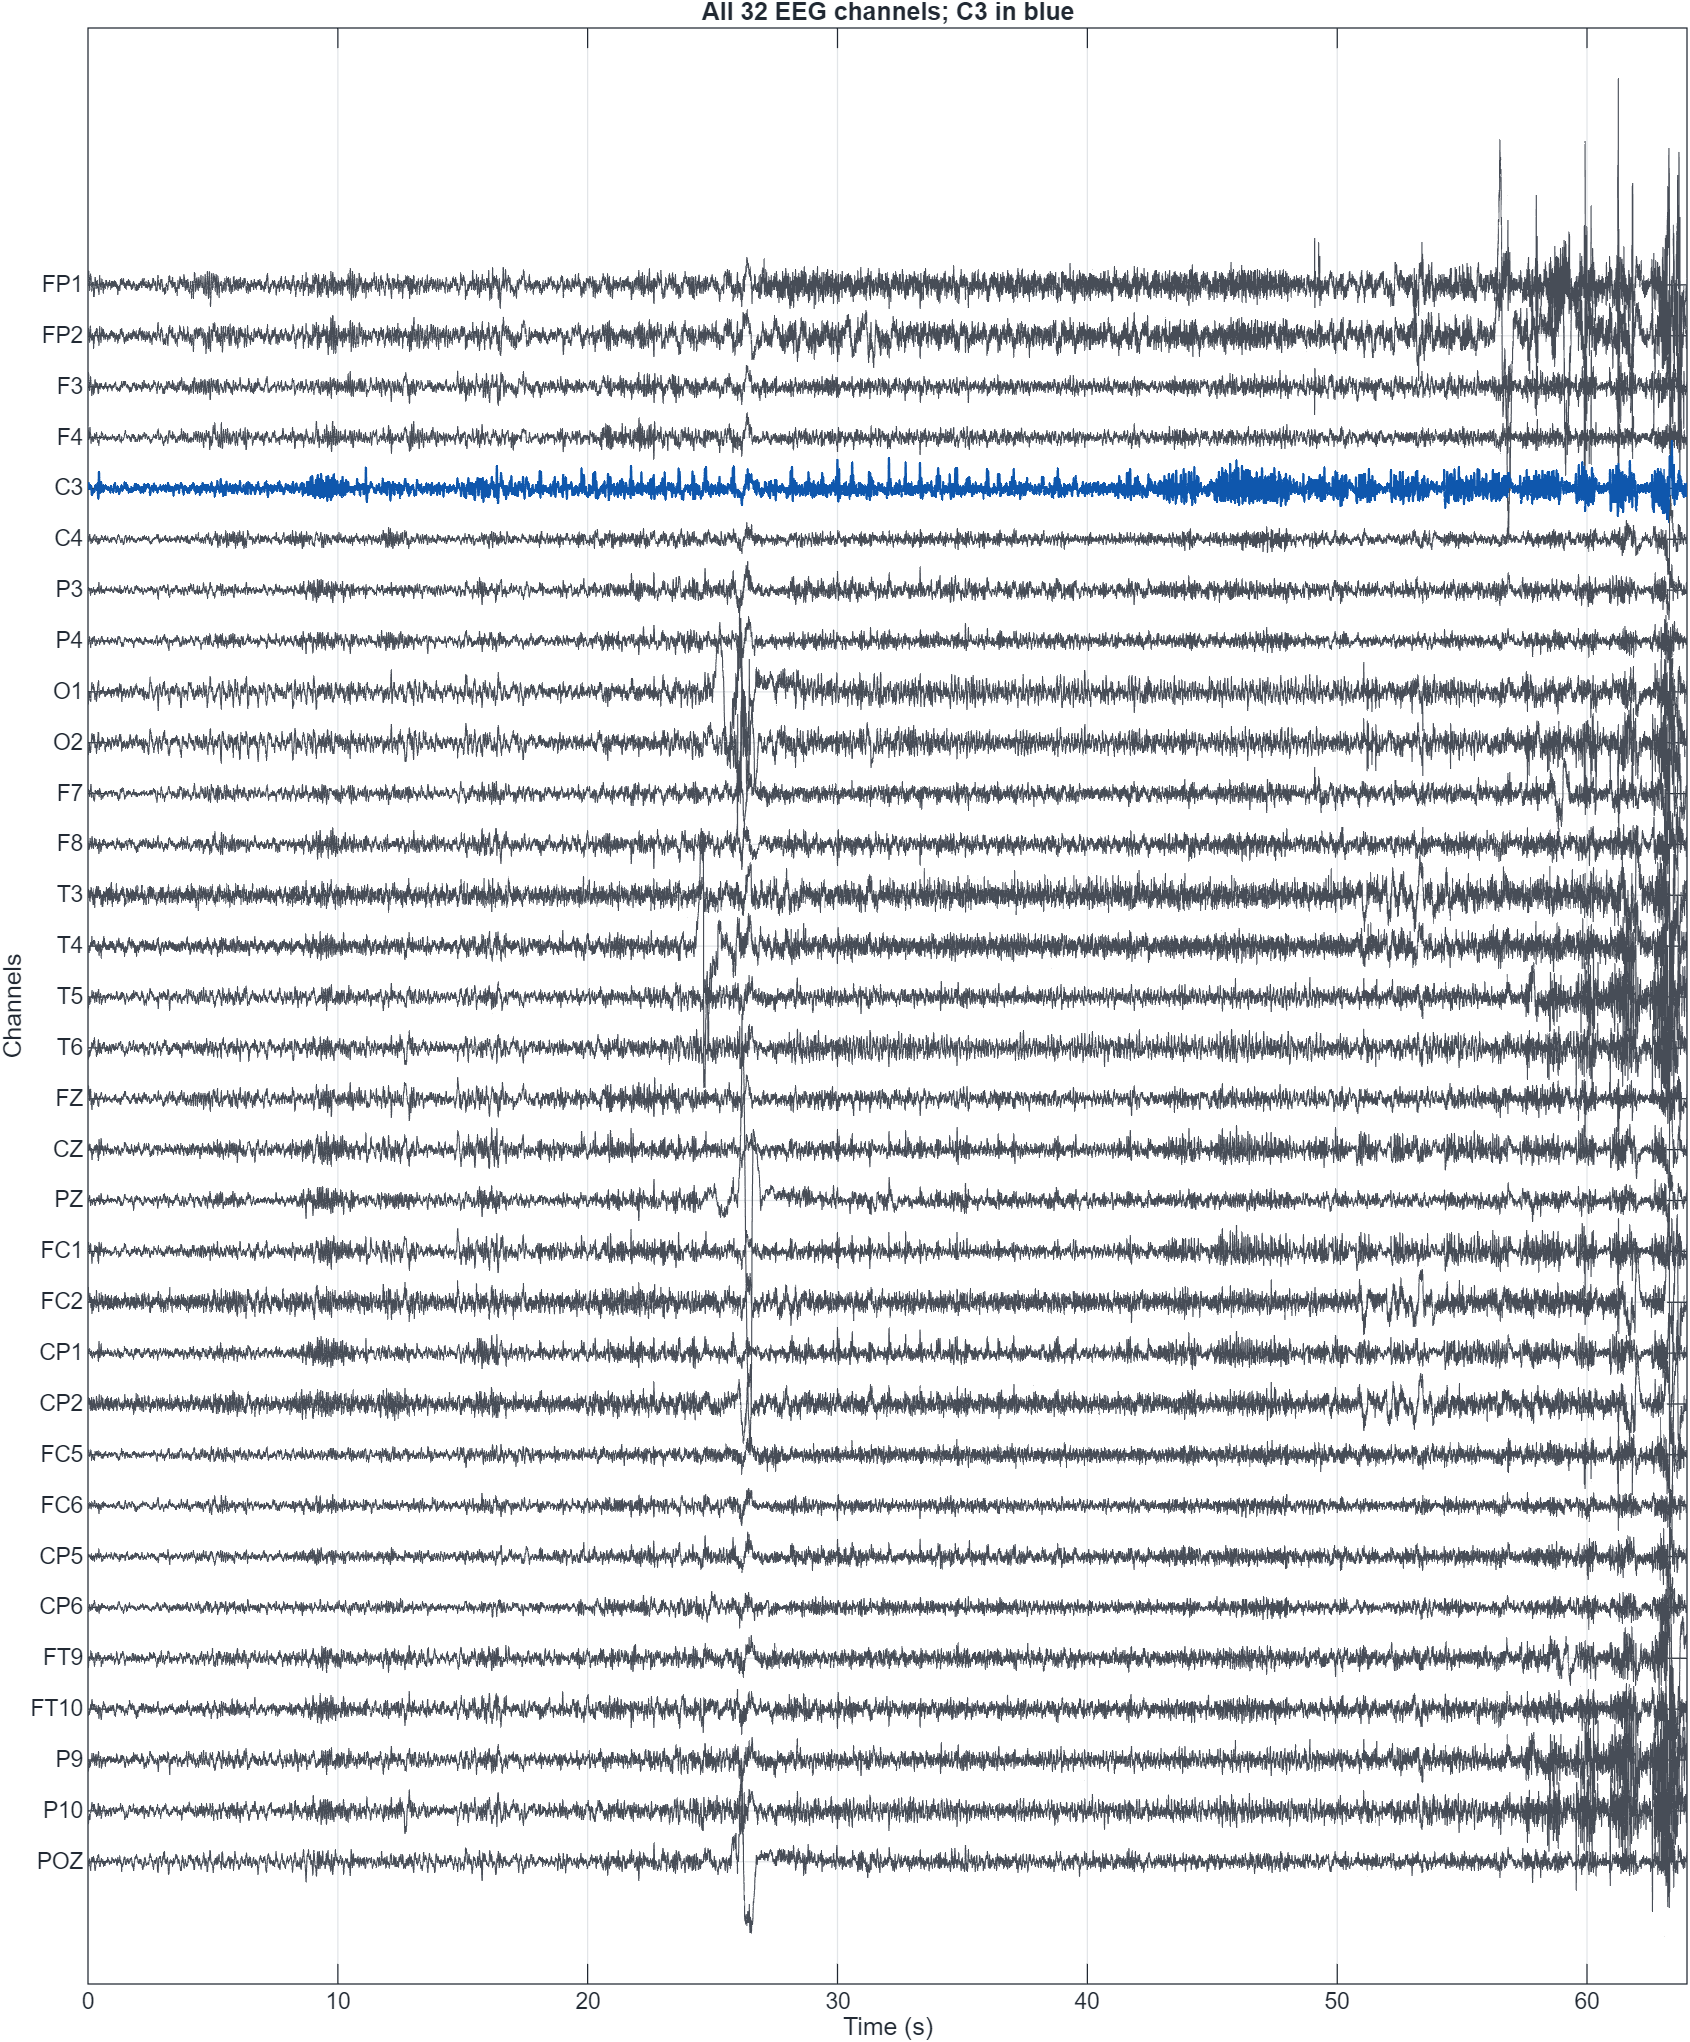
\includegraphics[height=0.78\textheight,keepaspectratio]{fig05_all_32_channels.png}
\caption{Display of all brain channels with a vertical offset, with the channel under study highlighted.}
\label{fig:all32}
\end{figure}

\subsection{Question 5: Interpreting the Three Sections of the Reference Figure}
\begin{taskbox}
Figure~1 of the manual shows the EEG signal of the first six channels. Research the characteristics of the signal in the three marked segments and summarize them briefly. (Caption of the manual's figure: a real EEG signal recorded from an epileptic patient during a seizure period, almost noise-free. Channel C3 shows seizure activity consisting of three parts: (1) rhythmic spikes before seizure onset (red box), (2) fast activity (green box) and (3) slower irregular activity (blue box).)
\end{taskbox}

\begin{figure}[H]
\centering
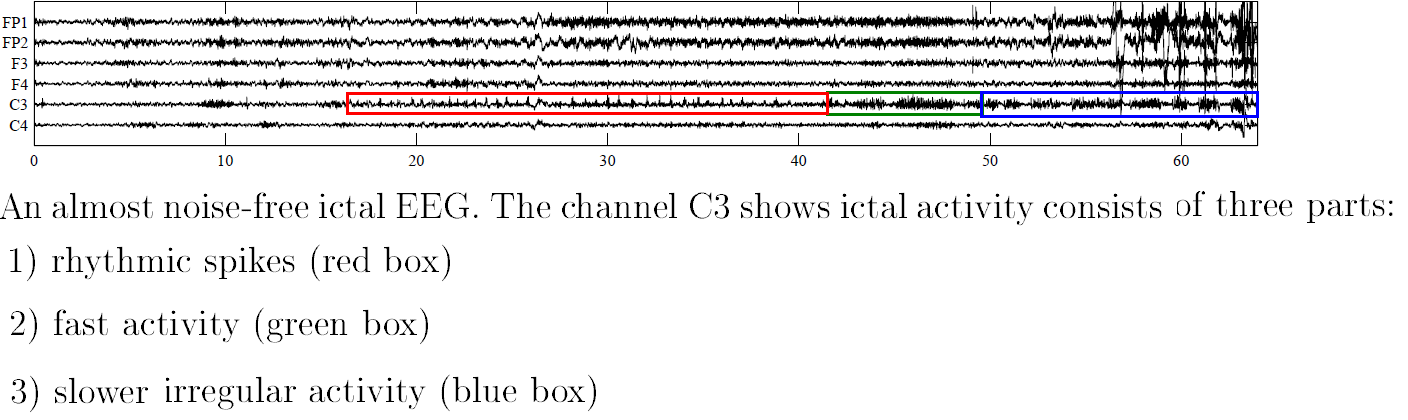
\includegraphics[width=\textwidth]{fig06_reference_ictal_figure.png}
\caption{The reference figure supplied with the data, for observing the three phases marked with colored frames. Its original caption reads: ``An almost noise-free ictal EEG. The channel C3 shows ictal activity consists of three parts: 1) rhythmic spikes (red box), 2) fast activity (green box), 3) slower irregular activity (blue box).''}
\label{fig:ref}
\end{figure}

Figure~\ref{fig:ref} is the reference image supplied with the experiment. The frame boundaries are approximate, and the three sections of channel C3 are interpreted on the basis of the waveform shape and its temporal evolution.

\paragraph{Red frame: rhythmic spikes before seizure onset.} At about 17 to 41.5 seconds, sharp, transient spikes repeat at relatively regular intervals. The title ``before seizure onset'' follows the Persian subtitle of the exercise statement; the exact electrographic onset of the seizure cannot be determined from the image alone. The repetition of the spikes creates periodicity, but their sharp shape also produces higher-frequency and harmonic components, so the repetition frequency is not the whole content of the spectrum. The presence of spikes alone is not sufficient for a definitive diagnosis or prediction of a seizure.

\paragraph{Green frame: fast activity.} At about 41.5 to 49.5 seconds, the oscillations become faster and more compact; their shorter temporal spacing is consistent with an increase in the higher-frequency content. The Welch peak at about 16.4~Hz and the larger beta share in the 42--47~s segment of the experiment data also support this description. Becoming faster is not necessarily an increase in amplitude; fast activity with low amplitude is also seen in some seizure-onset patterns.

\paragraph{Blue frame: slower and more irregular activity.} From about 49.5 seconds to the end, the activity is slower than in the green frame, and the spacing, shape and amplitude of the events are more variable. Slower components are prominent, but sharp transients can keep the spectrum broad. This part may be the evolution of the seizure activity itself; since the end of the attack is not marked and the exercise subtitle does not call it post-seizure, we do not take the slowing alone as equivalent to the end of the seizure.

The numerical values quoted here were computed from the data file, not from the image, and belong only to the corresponding segment. To compare intensity, the power or RMS must also be examined; a single spectral peak is not sufficient. The reference figure is described as almost noise-free, whereas the analyzed data contain artifacts; small differences between them are therefore not necessarily a contradiction.

\subsection{Question 6: Extracting Four Segments and the Fourier Transform}
\begin{taskbox}
Extract the following four 5-second segments from the C3 signal: 2 to 7~s, 30 to 35~s, 42 to 47~s and 50 to 55~s. Plot the time signal and the frequency spectrum (DFT) of each segment and give each figure a suitable title. Time and frequency must be displayed in seconds and Hz. Adjust the frequency axes so that the frequency content is displayed well (i.e., remove the high frequencies that carry no frequency information).
\end{taskbox}

Four segments, $(2,7]$, $(30,35]$, $(42,47]$ and $(50,55]$ seconds, were extracted. Each segment has exactly 1280 samples, and the spacing of the DFT points is 0.2~Hz. The mean was removed only for the spectral analysis. Figure~\ref{fig:dft4} shows the raw signal of each segment and its one-sided amplitude spectrum side by side. To see the main components, the frequency display is limited to 0--60~Hz; the full spectrum up to the Nyquist frequency is stored in the numeric file, and no display filter was applied.

\begin{figure}[H]
\centering
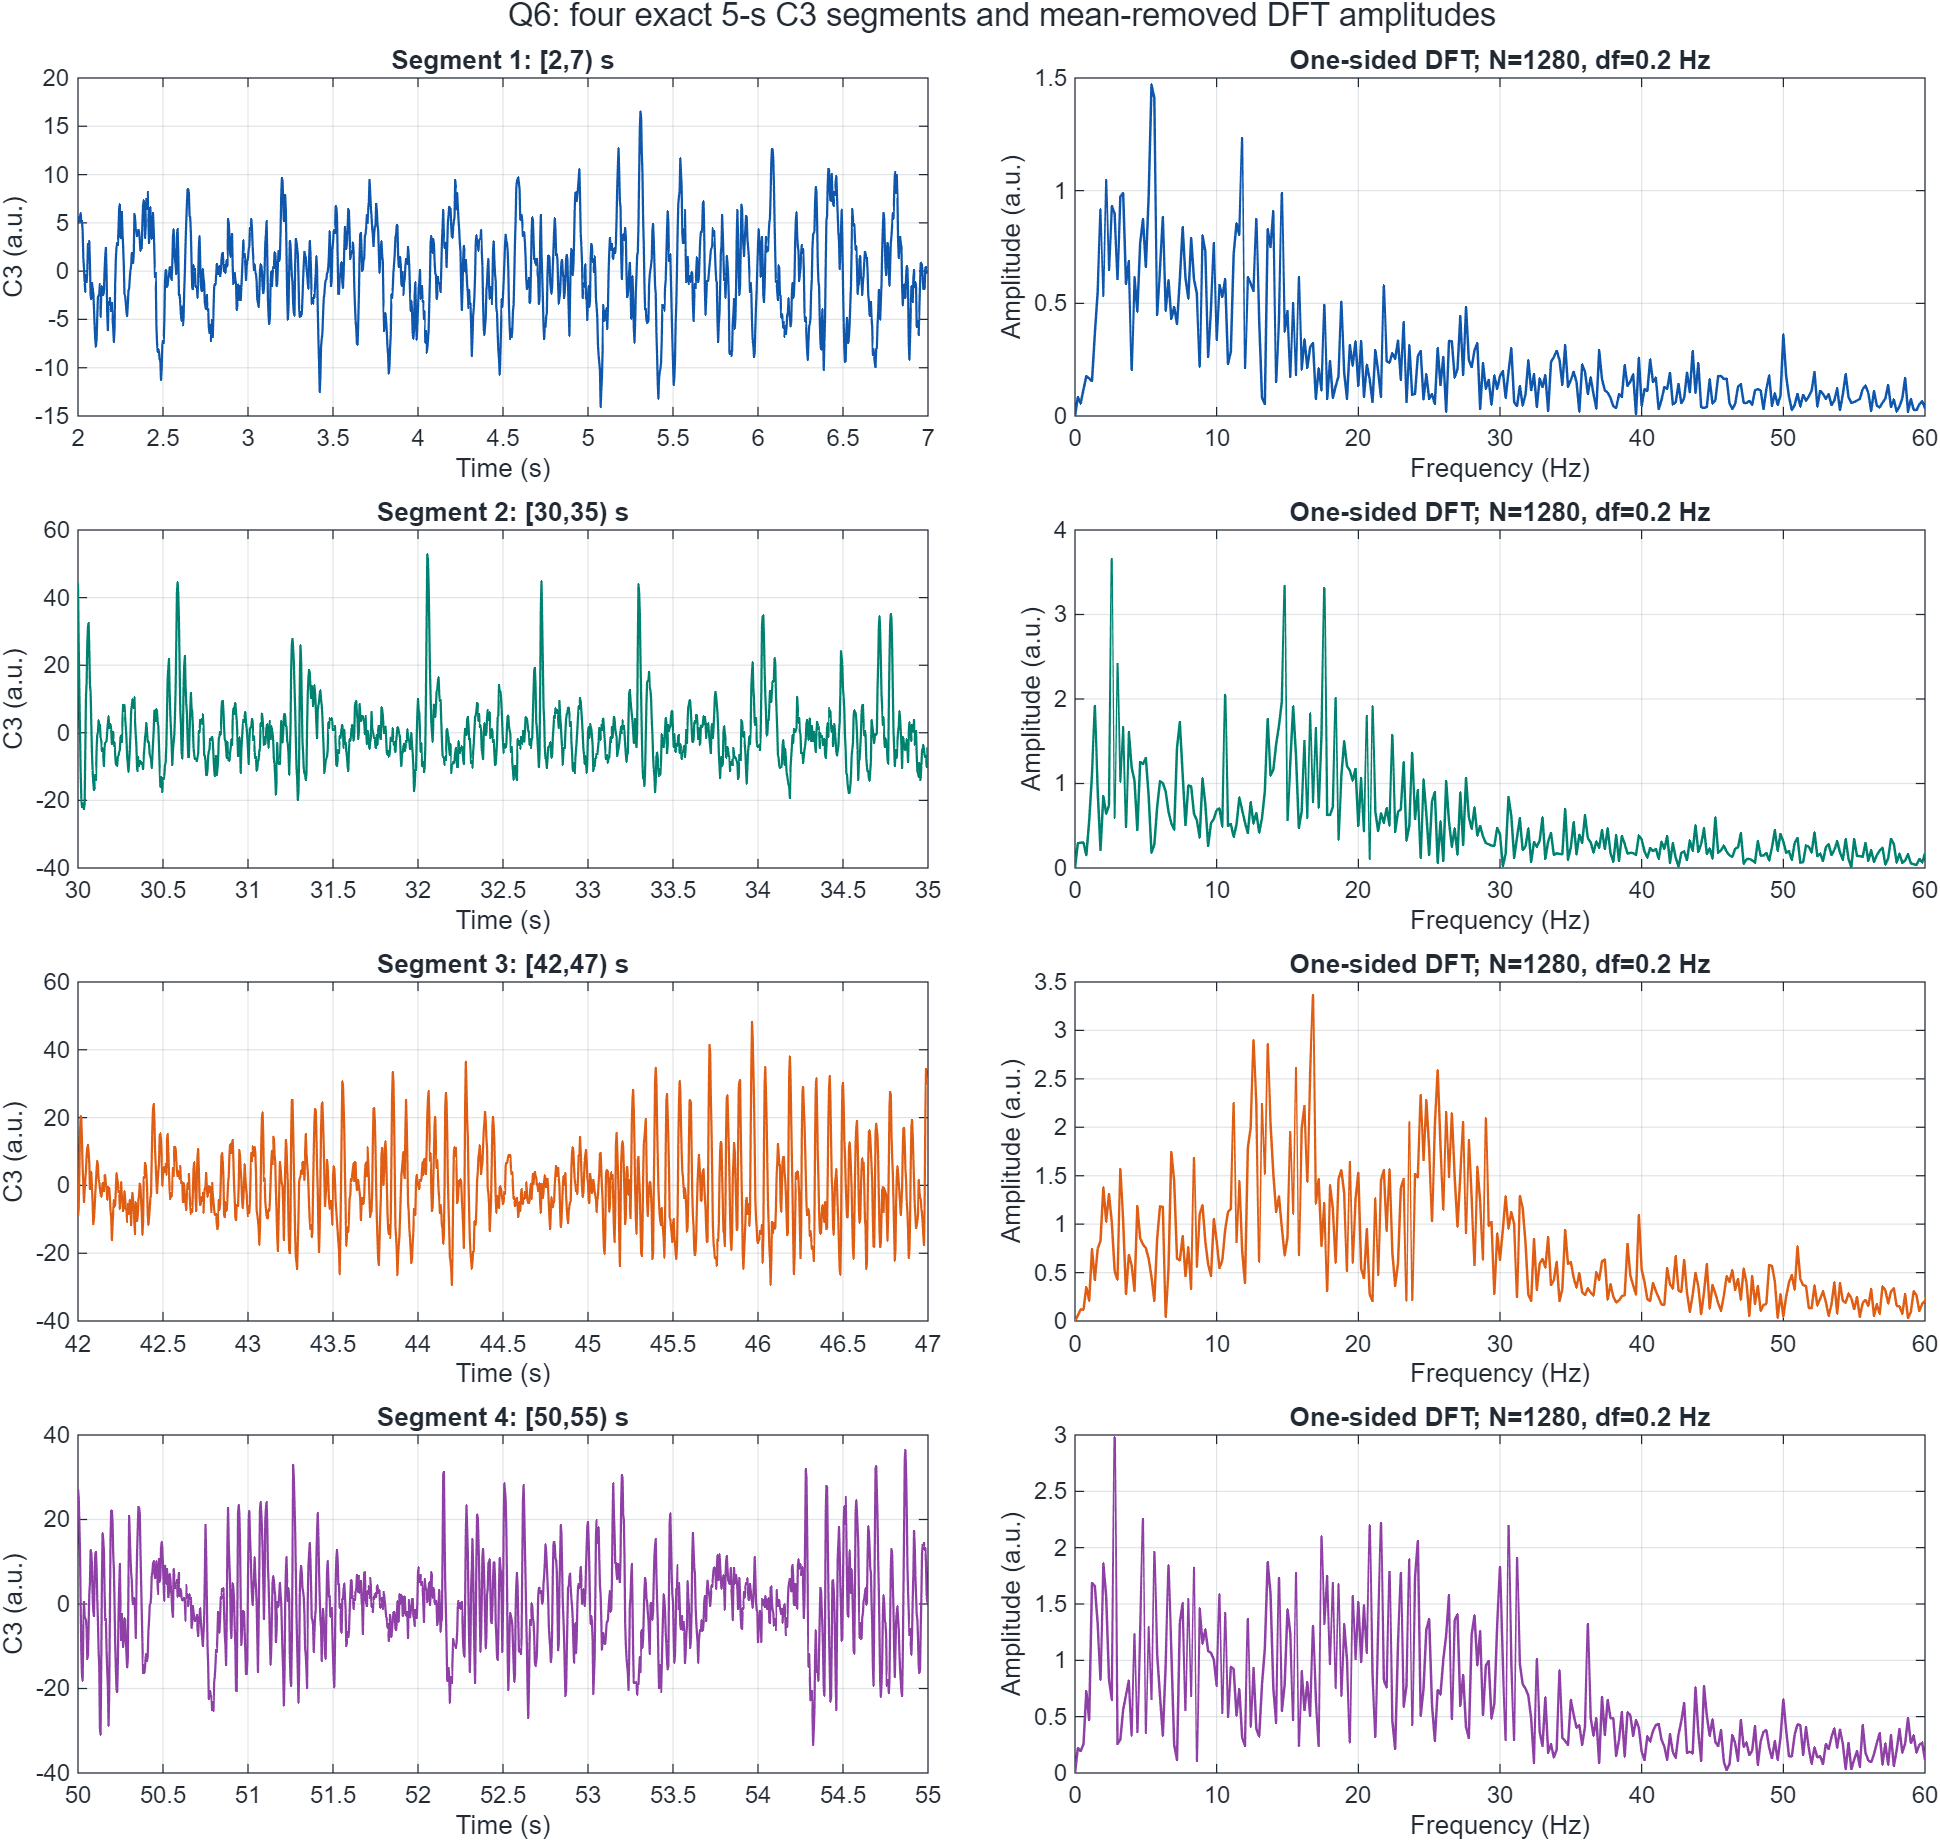
\includegraphics[width=\textwidth]{fig07_c3_segments_time_dft.png}
\caption{Time signal and amplitude spectrum of the four five-second segments with the correct DFT scaling.}
\label{fig:dft4}
\end{figure}

\subsection{Question 7: Spectrum Estimation with Welch's Method}
\begin{taskbox}
Plot the frequency spectrum of each of the four segments using the function \texttt{pwelch.m}. Set the input parameters so that the frequency content is displayed well. What can be said about the frequency characteristics of each of the four segments?
\end{taskbox}

For \texttt{pwelch}, a Hamming window of length 256, an overlap of 128 and \texttt{nfft=2048} at 256~Hz were used. Nine windows are averaged in each segment. The spacing of the plotting grid is 0.125~Hz; the intrinsic resolution of a one-second window remains of the order of 1~Hz. Besides the spectral peaks, Figure~\ref{fig:welch4} shows the increase in power of the second and third segments.

\begin{figure}[H]
\centering
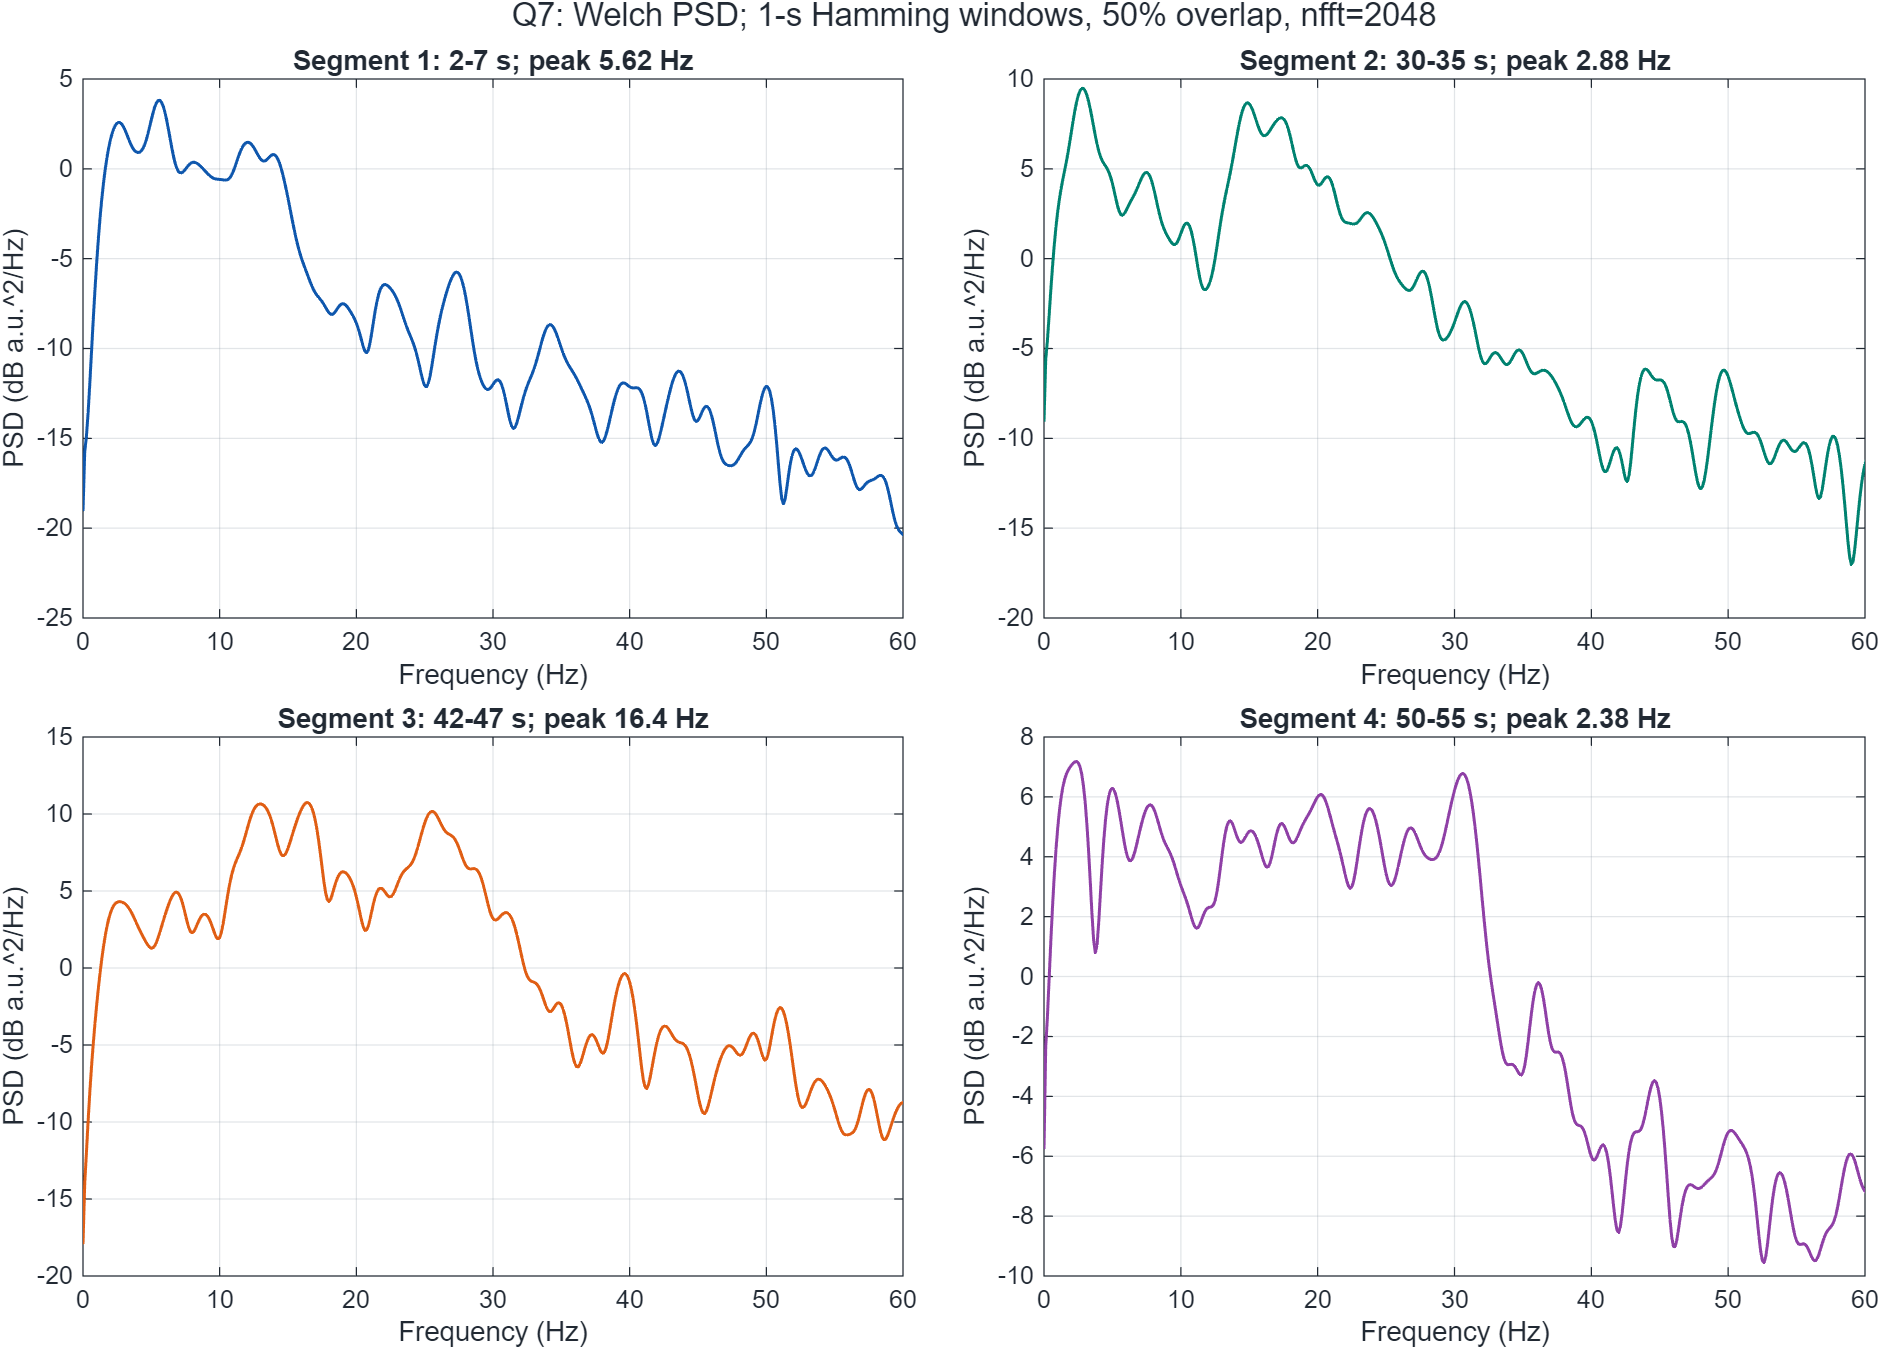
\includegraphics[width=0.95\textwidth]{fig08_welch_psd_segments.png}
\caption{Power spectral density of the four segments with fixed Welch settings.}
\label{fig:welch4}
\end{figure}

\begin{center}
\begin{tabular}{@{}ccccc@{}}
\toprule
\textbf{Interval (s)} & \textbf{AC RMS} & \textbf{Welch peak (Hz)} & \textbf{Beta share (\%)} & \textbf{Power above 60~Hz (\%)}\\
\midrule
2--7   &  4.58 &  5.625 & 21.97 & 1.44\\
30--35 &  9.61 &  2.875 & 52.92 & 2.09\\
42--47 & 12.14 & 16.375 & 64.82 & 1.72\\
50--55 & 10.81 &  2.375 & 47.32 & 2.71\\
\bottomrule
\end{tabular}
\end{center}

The beta share in the table was computed as the integral of power from 13 to 30~Hz divided by the power from 0.5 to 100~Hz. The share in the last column is relative to the total Welch power up to 128~Hz. These two denominators are different, and the values do not add up.

In the first segment, the main peak is at about 5.625~Hz, and the energy is distributed among the lower bands. In the second segment, the 2.875~Hz peak is consistent with the slow repetition of the spikes, but more than half of the power in the 0.5--100~Hz range lies in the beta band; the main peak alone therefore does not describe the width of the spectrum. The third segment has a peak at 16.375~Hz and a beta share of about 64.82\%, and it shows the fast activity more clearly. The peak of the fourth segment returns to 2.375~Hz, but the fast content and the artifacts have not completely disappeared.

\subsection{Question 8: Spectrogram with the Specified Settings}
\begin{taskbox}
Using the \texttt{spectrogram} command with window length $L=128$, an overlap of $N_{\mathrm{overlap}}=64$ points and $n_{\mathrm{fft}}=L=128$, compute and plot the time--frequency spectrum of the four segments using a Hamming window (time and frequency axes in seconds and Hz, respectively). What can be said about the time--frequency characteristics of each of the four segments?
\end{taskbox}

The parameters were set exactly to $L=128$, $N_{\mathrm{overlap}}=64$, $n_{\mathrm{fft}}=128$ and a Hamming window. As a result, the window length is 0.5~s, the time step is 0.25~s and the frequency spacing is 2~Hz. Each segment has 19 time frames. The color in Figure~\ref{fig:stft4} is in decibels of power spectral density, with common limits in all panels.

\begin{figure}[H]
\centering
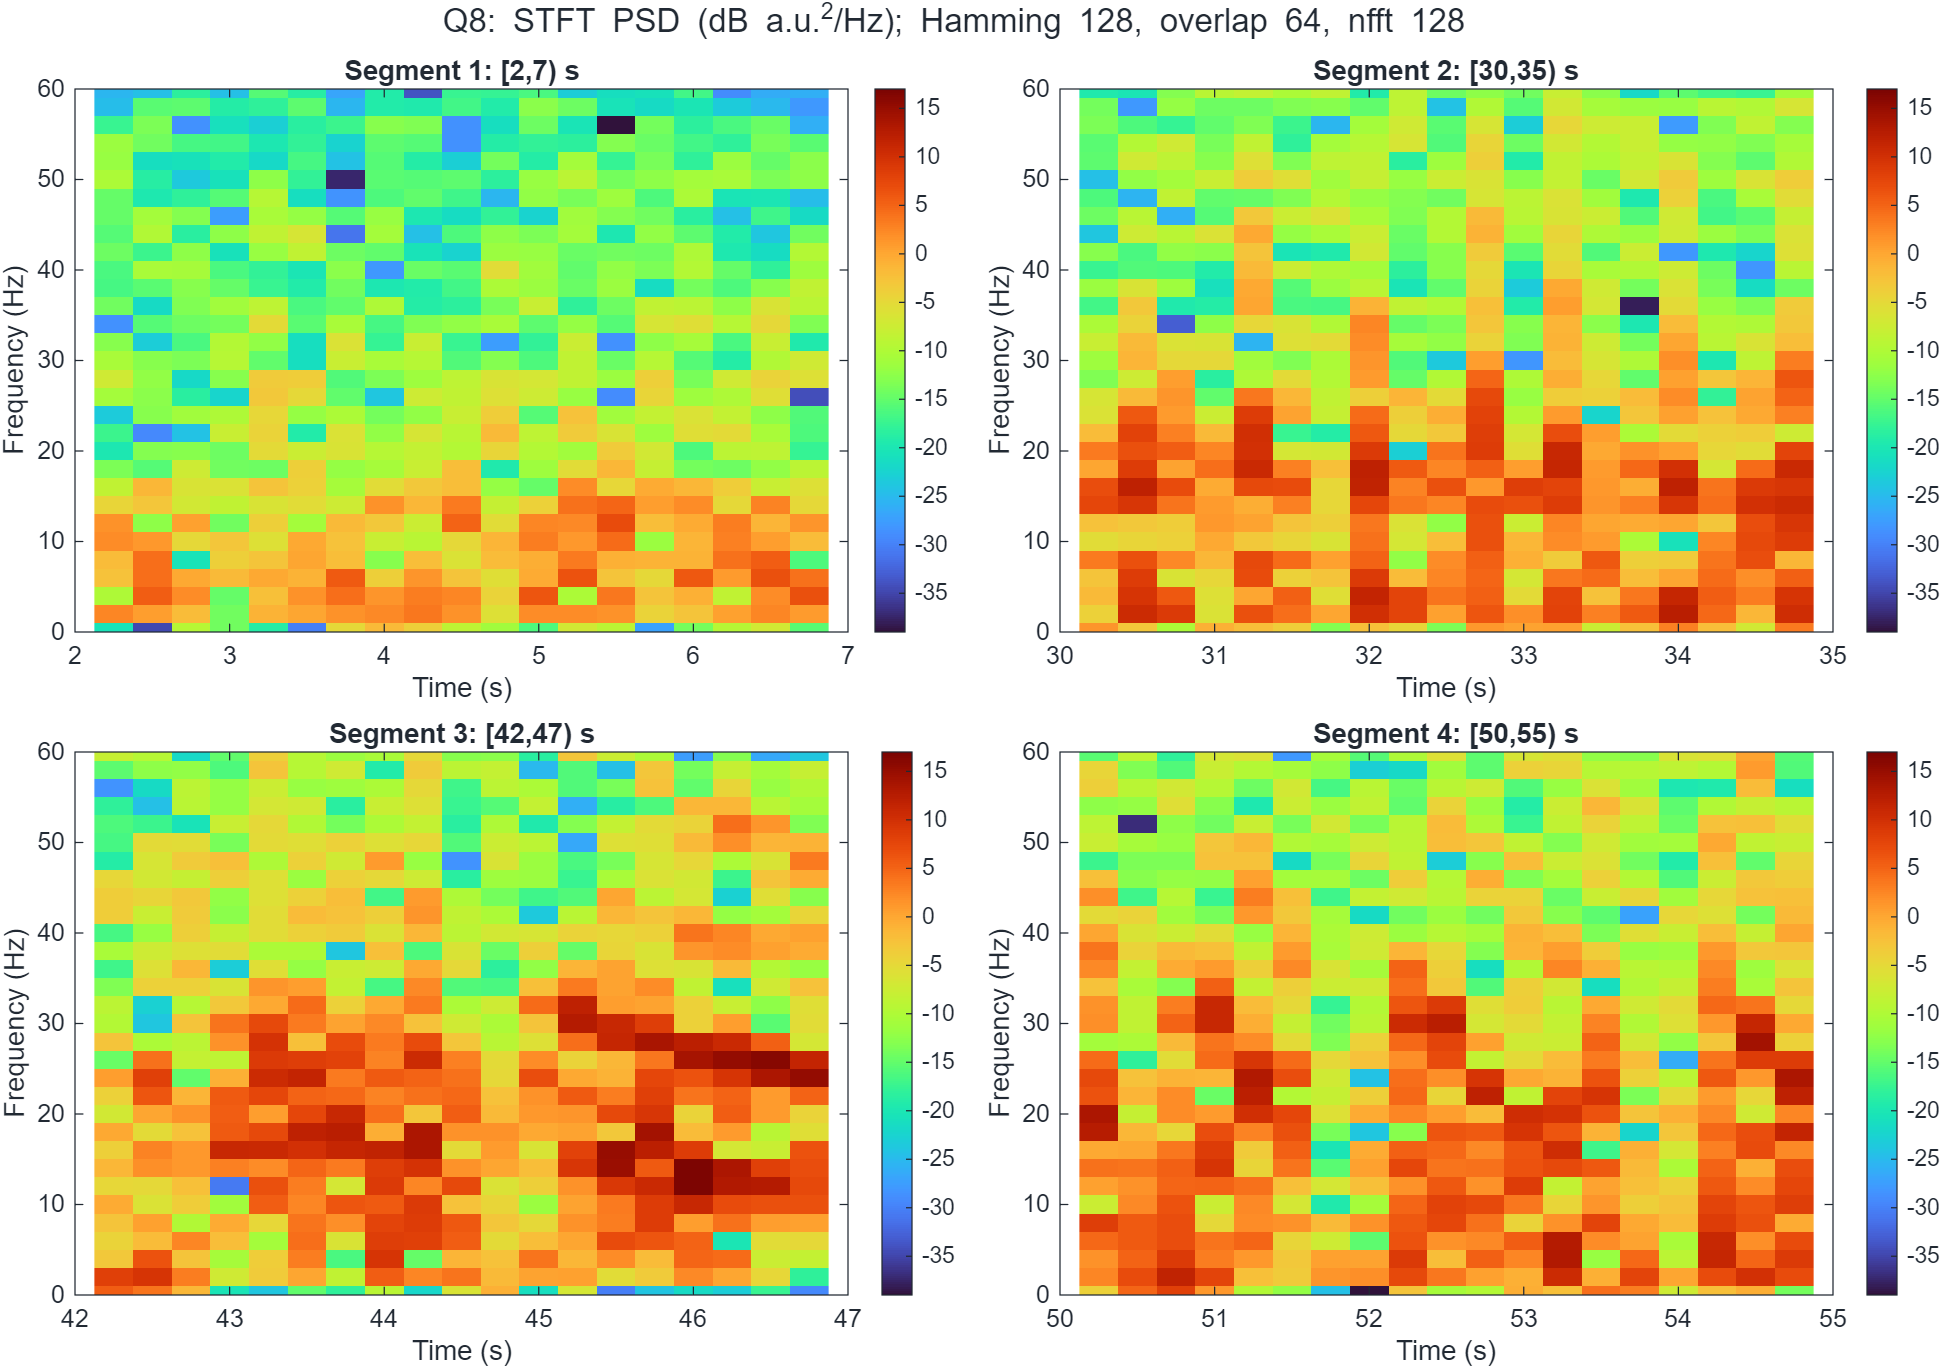
\includegraphics[width=0.95\textwidth]{fig09_stft_segments.png}
\caption{Spectrogram of the four segments with the exactly requested window and overlap.}
\label{fig:stft4}
\end{figure}

\answer In the first segment, the power is lower and the activity has a smaller amplitude. The second segment shows repeating temporal variations and the simultaneous presence of slow and fast components; the wide-band transient stripes are consistent with the sharpness of the spikes. In the third segment, the energy in the beta range and around 16~Hz is more prominent. In the fourth segment, the distribution of power is more irregular, and slow components are accompanied by fast transients. This display shows that two segments with similar overall spectra can have different temporal ordering; a stationary spectrum alone does not reveal this difference.

\subsection{Question 9: Reducing the Sampling Rate and Checking Information Preservation}
\begin{taskbox}
Consider the signal of segment 2. Since the sampling frequency is relatively high, assume that the obtained frequency spectrum is similar to the spectrum of the continuous signal. Under this assumption, and using the information obtained in Questions 6 and 7, reduce the sampling frequency (downsampling) such that the frequency content is preserved. Before reducing the sampling rate, use a suitable low-pass filter. Plot the time signal, the frequency spectrum (DFT) and the STFT of the new signal, and compare them with the results of the previous parts.
\end{taskbox}

For the second segment, downsampling by a factor of two, from 256 to 128~Hz, was chosen. In the raw recording, the power above the new Nyquist frequency is not zero: about 1.85\% of the Welch power lies above 64~Hz, and the bandwidth containing 99\% of the power is about 84.5~Hz. Complete preservation of the full bandwidth of the recording at 128~Hz is therefore not possible. The purpose of this choice is an approximate preservation of the main brain band and a controlled reduction of the fast content of the recording.

A low-pass filter with a passband edge of 48~Hz, a stopband start of 64~Hz, a single-pass ripple of 0.1~dB and a single-pass attenuation of 60~dB was designed. \texttt{filtfilt} was run on the whole channel, then every other sample was kept, and finally the same time interval was extracted. In this way, the two edges of the segment use the actual neighboring samples for filtering, and the forward--backward phase delay is removed. The effective amplitude response is the square of the single-pass response; a maximum passband deviation of about 0.170~dB and a stopband attenuation of about 120~dB were measured.

\begin{center}
\begin{tabular}{@{}lr@{}}
\toprule
\textbf{Index} & \textbf{Value}\\
\midrule
Number of samples before / after the reduction & 1280 / 640\\
Duration of both segments (s) & 5\\
Share of the main power below 48~Hz & 96.56\%\\
Ratio of the filtered time-domain power to the raw & 97.14\%\\
Correlation with the corresponding raw samples & 0.9862\\
Relative difference of the Welch spectrum in 0.5--40~Hz & 0.327\%\\
Relative difference of the spectrogram below 40~Hz & 1.462\%\\
\bottomrule
\end{tabular}
\end{center}

The correlation of about 0.986 and the difference of about 0.327\% in the Welch spectrum in the 0.5--40~Hz band show that the main part of the oscillations was preserved. The difference from the raw data is intentionally non-zero; the RMSE of the retained samples is about 1.609~a.u. We therefore do not claim a lossless reconstruction for the whole recording. Figure~\ref{fig:ds} presents the comparison of time, amplitude, power density and the filter response.

\begin{figure}[H]
\centering
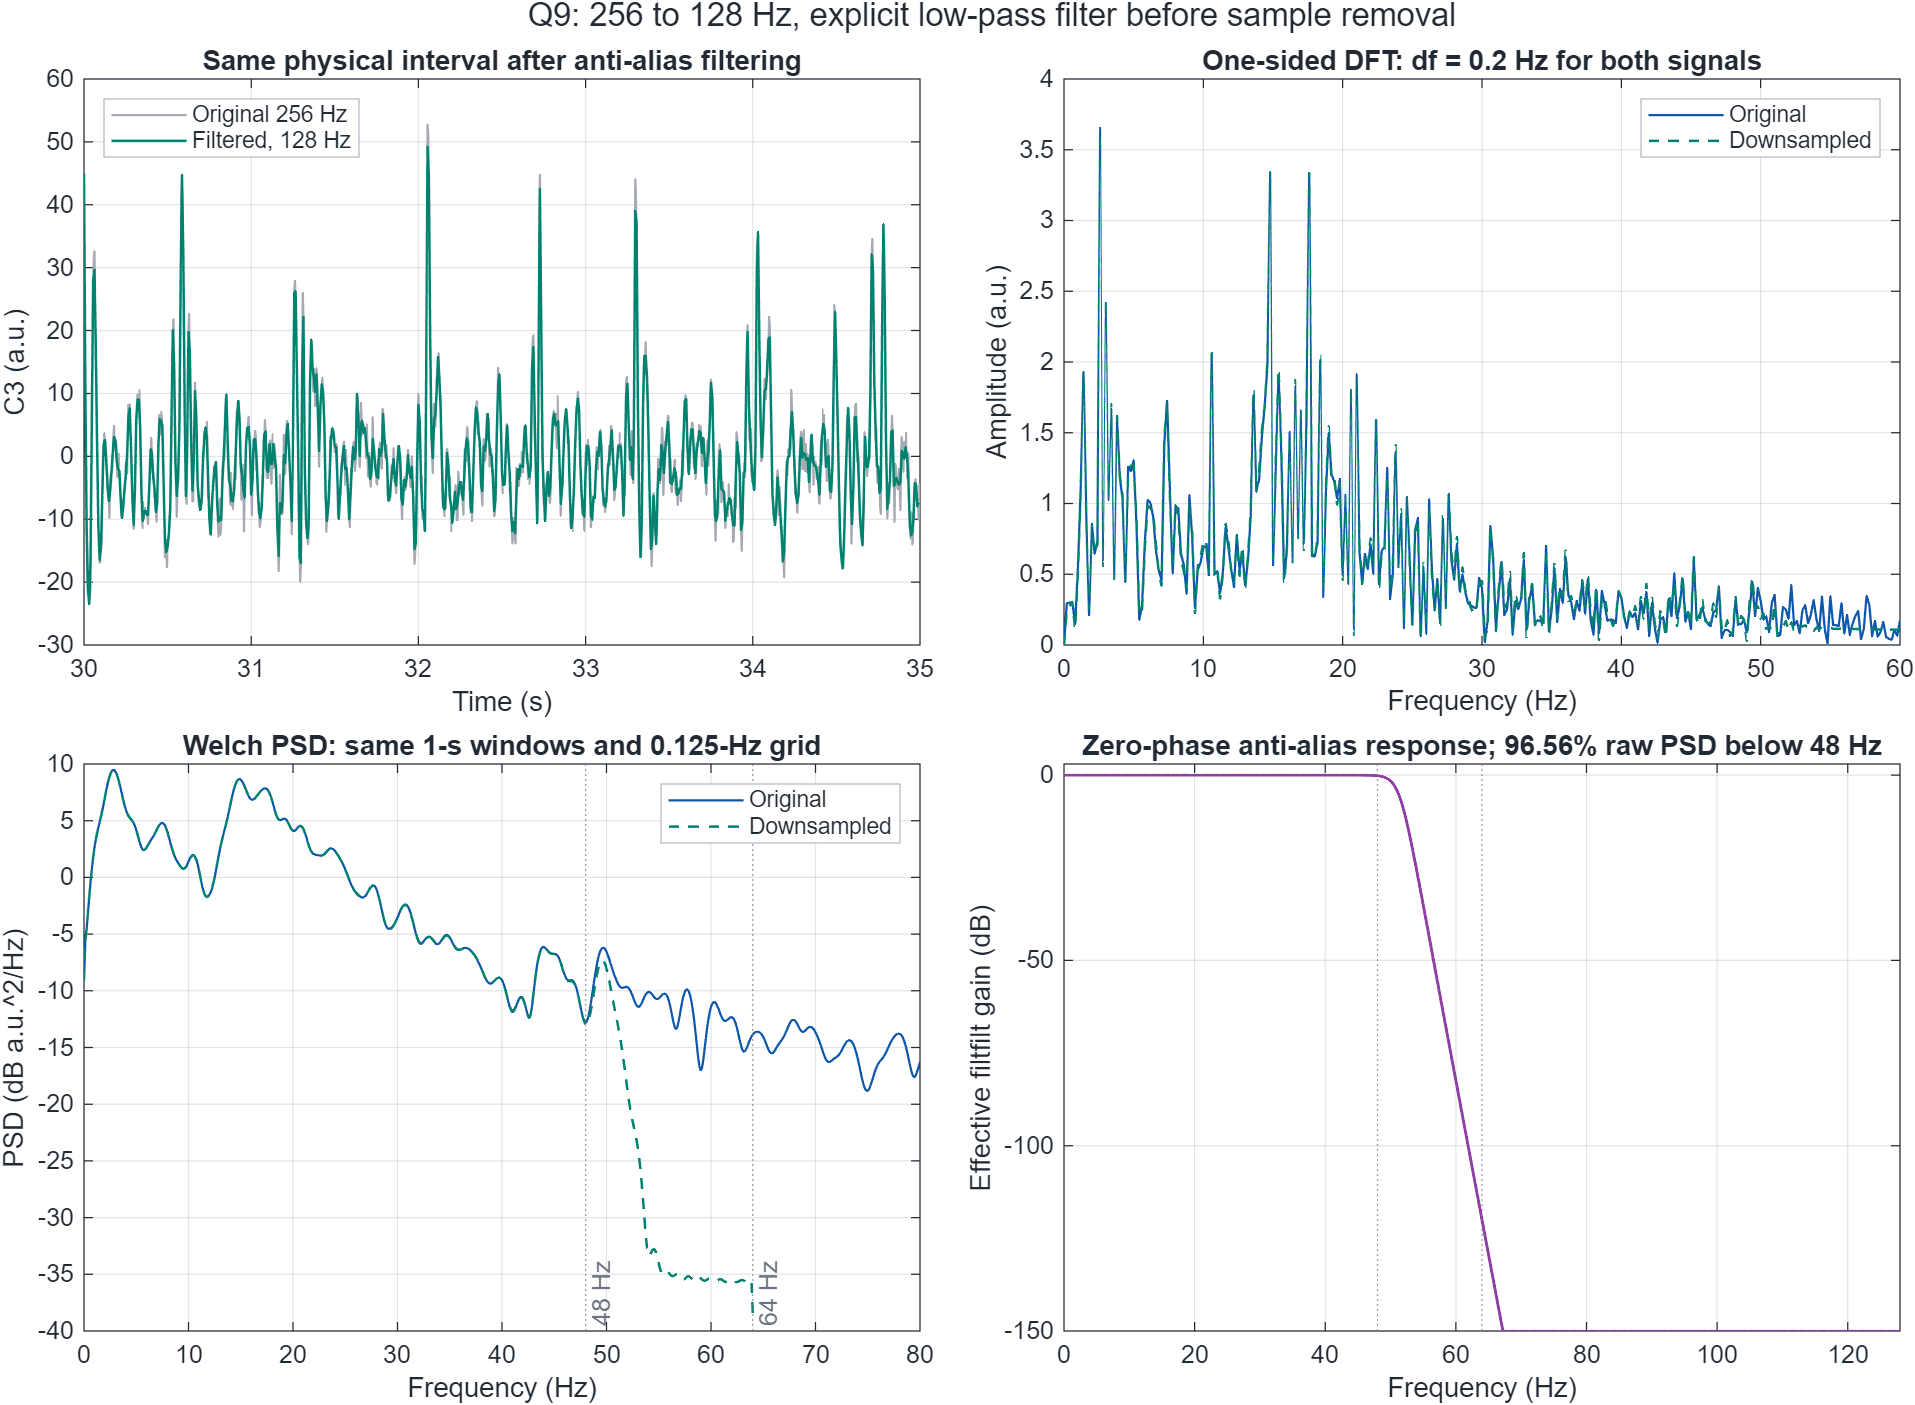
\includegraphics[width=\textwidth]{fig10_downsampling_comparison.png}
\caption{Comparison before and after reducing the sampling rate, and examination of the anti-aliasing filter response.}
\label{fig:ds}
\end{figure}

For a fair comparison of time and frequency, the physical length of the window was kept fixed. At the new rate, the spectrogram window has 64 samples, an overlap of 32 and \texttt{nfft=64}; the window is therefore still half a second long and the frequency spacing is still 2~Hz. Reusing the length of 128 samples at the new rate would have made the window one second long and mixed the effect of the rate reduction with the effect of changing the window. Figure~\ref{fig:dsstft} shows the similarity of the original time--frequency pattern on compatible grids.

\begin{figure}[H]
\centering
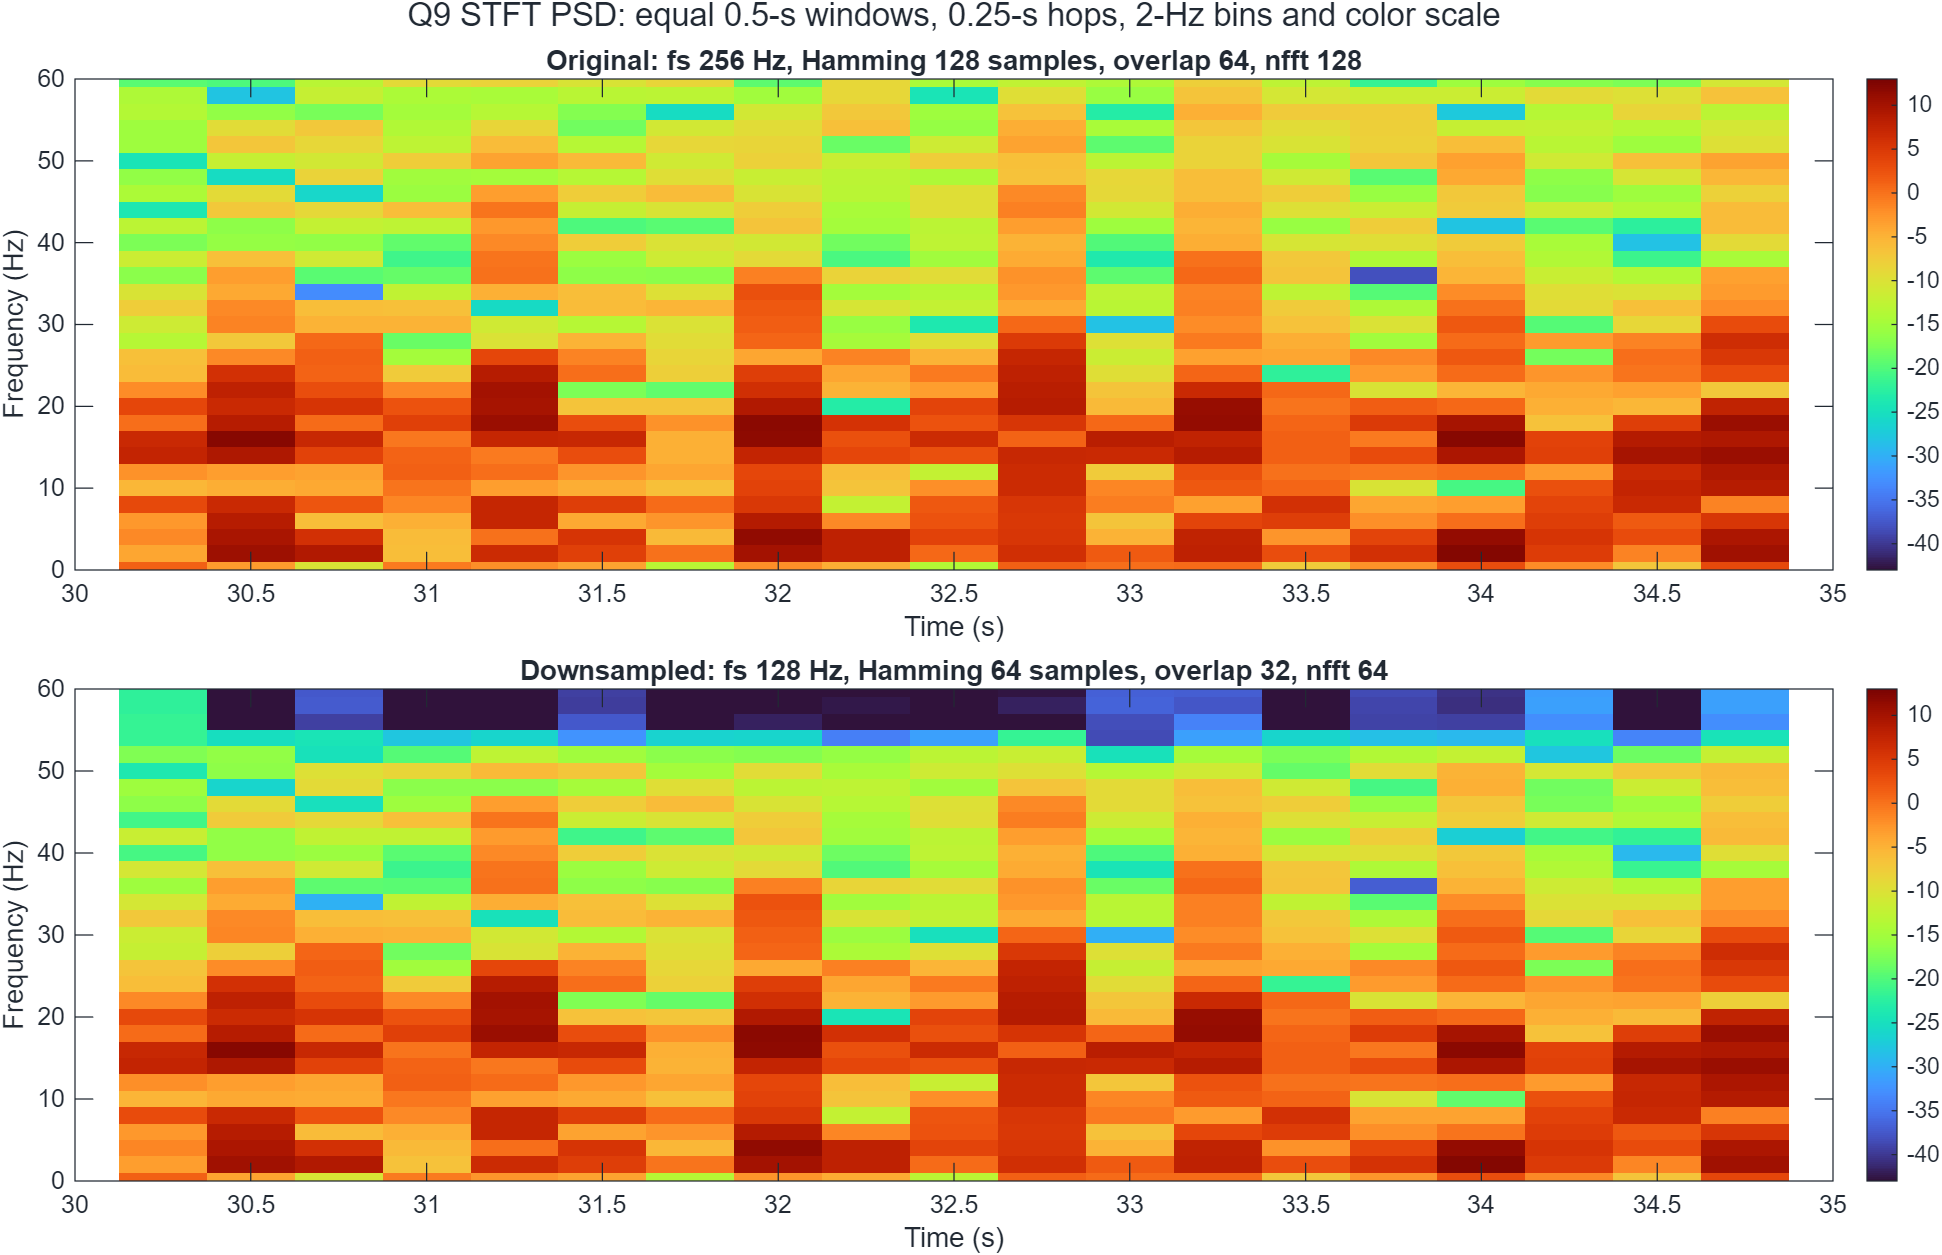
\includegraphics[width=0.95\textwidth]{fig11_stft_before_after_downsampling.png}
\caption{Comparison of the spectrogram before and after the reduction, with the same window duration and a common color scale.}
\label{fig:dsstft}
\end{figure}

\subsection{Core Implementation (EEG)}

\begin{lstlisting}[language=Matlab]
fs = des.samplingfreq;
t = (0:size(Z,2)-1)/fs;
idx = round(30*fs)+1 : round(35*fs);
x = Z(5,idx);                      % Exactly 1280 samples
[P,f] = pwelch(x-mean(x),hamming(256),128,2048,fs);
[S,F,T,Ptf] = spectrogram(x-mean(x),hamming(128),64,128,fs);
\end{lstlisting}

The motivation for this code is to avoid a one-sample error in slicing and to build the frequency axis from the actual recording rate. The complete code for filtering, extracting the indices and saving the figures is in \texttt{code/lab1\_eeg.m}.

\section{Part 2: Cardiac Signal (ECG)}

\begin{taskbox}[Part 2: introduction in the lab manual]
A segment of ECG recorded from two leads is provided in the file \texttt{sig\_ECG.mat}. This signal is record number 201 of the MIT-BIH Arrhythmia database. More details about this database can be found in the file \texttt{Introduction\_Arrhythmia.pdf}. The signals recorded in this database belong to healthy and diseased subjects over a duration of 30 minutes, and the R-peak location and the label of each beat (normal/abnormal and its type) are specified.
\end{taskbox}

\subsection{Question 1: Displaying Two Leads and Comparing Beat Shapes}
\begin{taskbox}
Plot the signals of the two channels in time (stored in the matrix \texttt{Sig} with sampling frequency \texttt{sfreq}). The time axis must be displayed in seconds. By zooming on the horizontal axis, examine the changes of the signals of the two channels over time. Are the beats similar to each other over time in each channel? Are the beats of the two channels similar? Plot two sample (different) beats and mark the P, Q, R, S and T waves on them.
\end{taskbox}

The cardiac data belong to record 201 of the MIT-BIH Arrhythmia database. According to the original header, the two leads are MLII and V1, and the sampling rate is 360~Hz. The stored amplitude is consistent with a calibration of 200~ADU/mV and a baseline of 1024; for example, the initial digital values 972 and 982 convert to $-0.26$~mV and $-0.21$~mV, which match the first row of the data. The amplitude axis of this part is therefore in millivolts.

\begin{figure}[H]
\centering
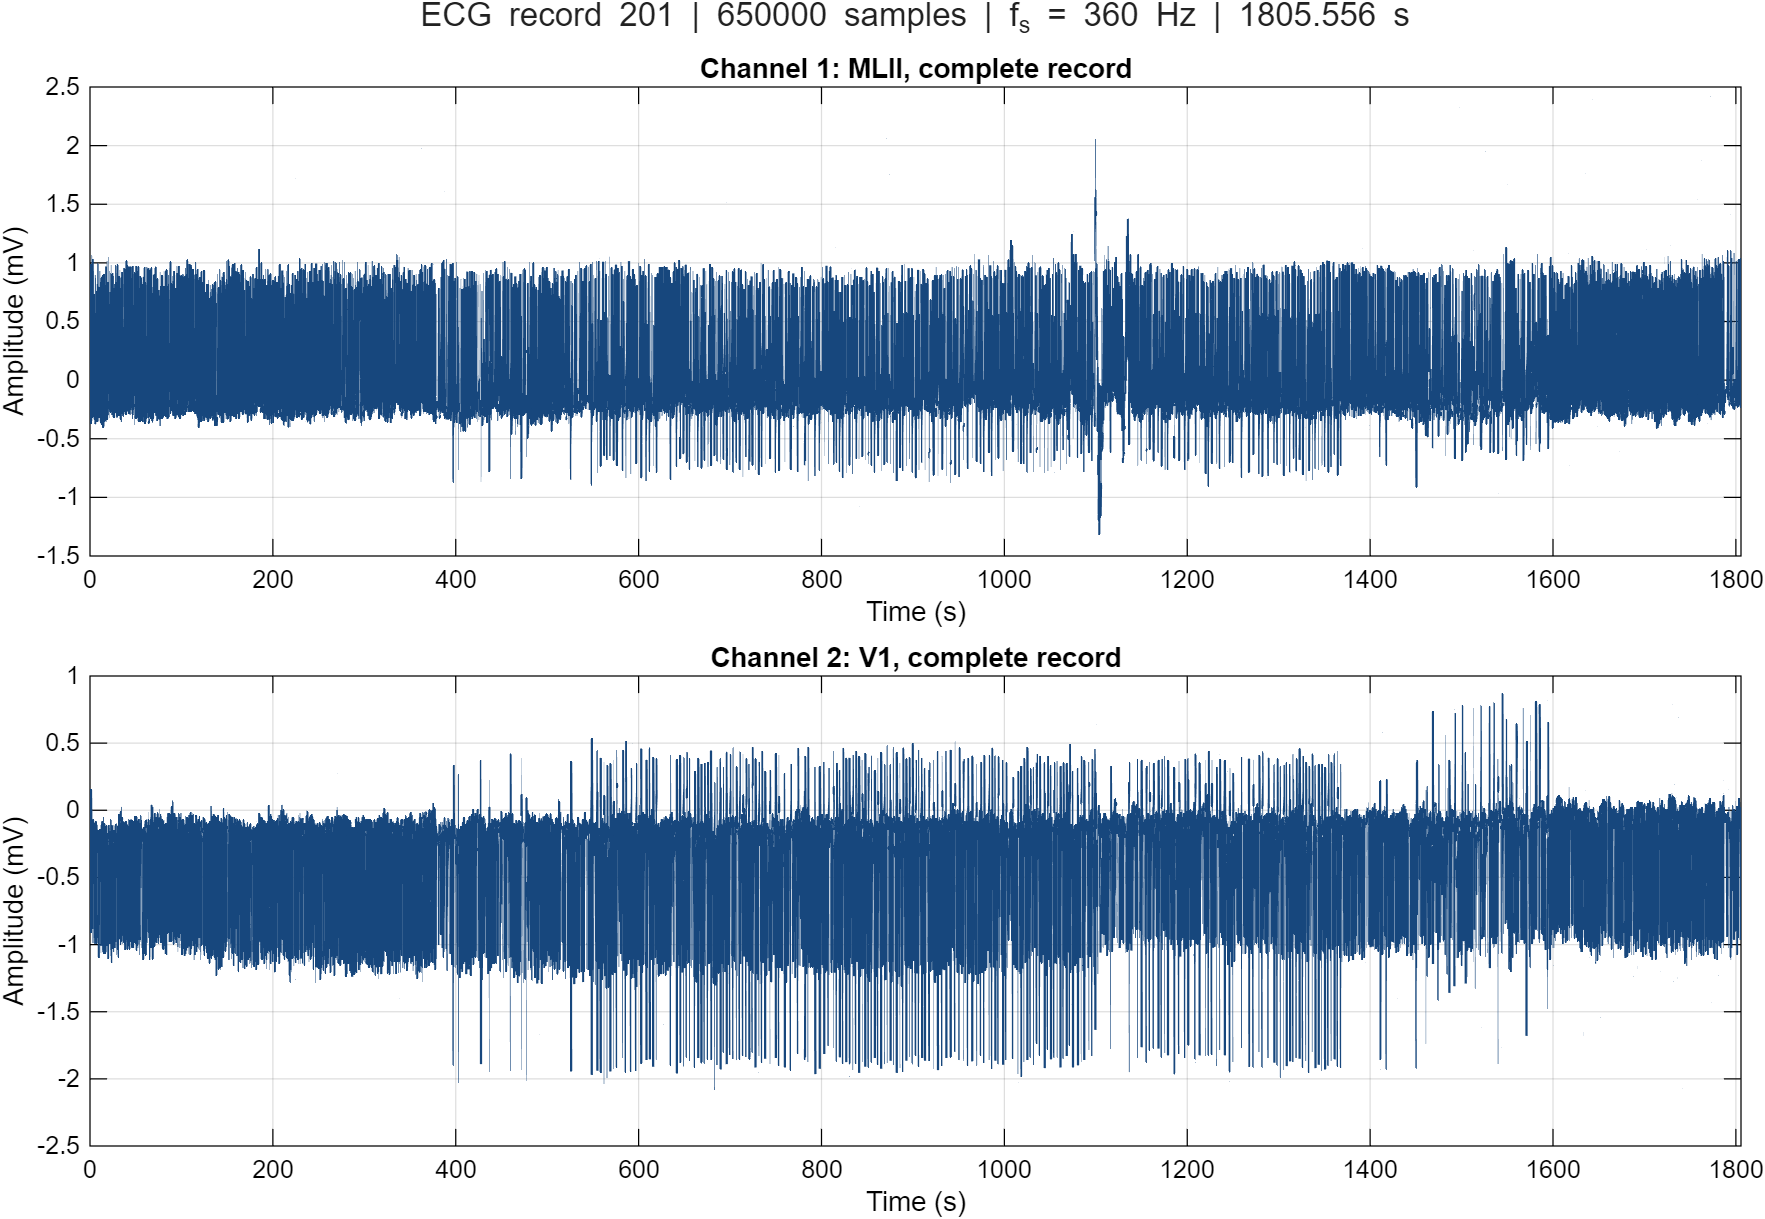
\includegraphics[width=0.95\textwidth]{fig12_ecg_full_record.png}
\caption{Complete recording of the two cardiac leads, with the time axis reconstructed from the real length of the signal.}
\label{fig:ecgfull}
\end{figure}

Figure~\ref{fig:ecgfull} gives the overall view of the recording, and Figure~\ref{fig:ecgseg} shows enlarged segments. The time of occurrence of the cardiac complexes is common to the two leads, because both record the same heart; the shape, amplitude and polarity, however, are not the same. In MLII a positive R wave is usually prominent, whereas in V1 a small r and a larger negative S component are seen. The change of the viewing axis and the location of the electrodes explain this difference.

The beats of a single lead are also not completely similar over the whole recording. At the start of the recording the intervals are irregular, at about 397.6 seconds there is a ventricular sample with a different shape, and at about 1430 seconds several beats with N shape are seen more regularly. The N label specifies the usual shape of the complex; by itself it does not mean sinus rhythm or the health of the whole recording. According to the original description of the data, the recording begins with atrial fibrillation.

\begin{figure}[H]
\centering
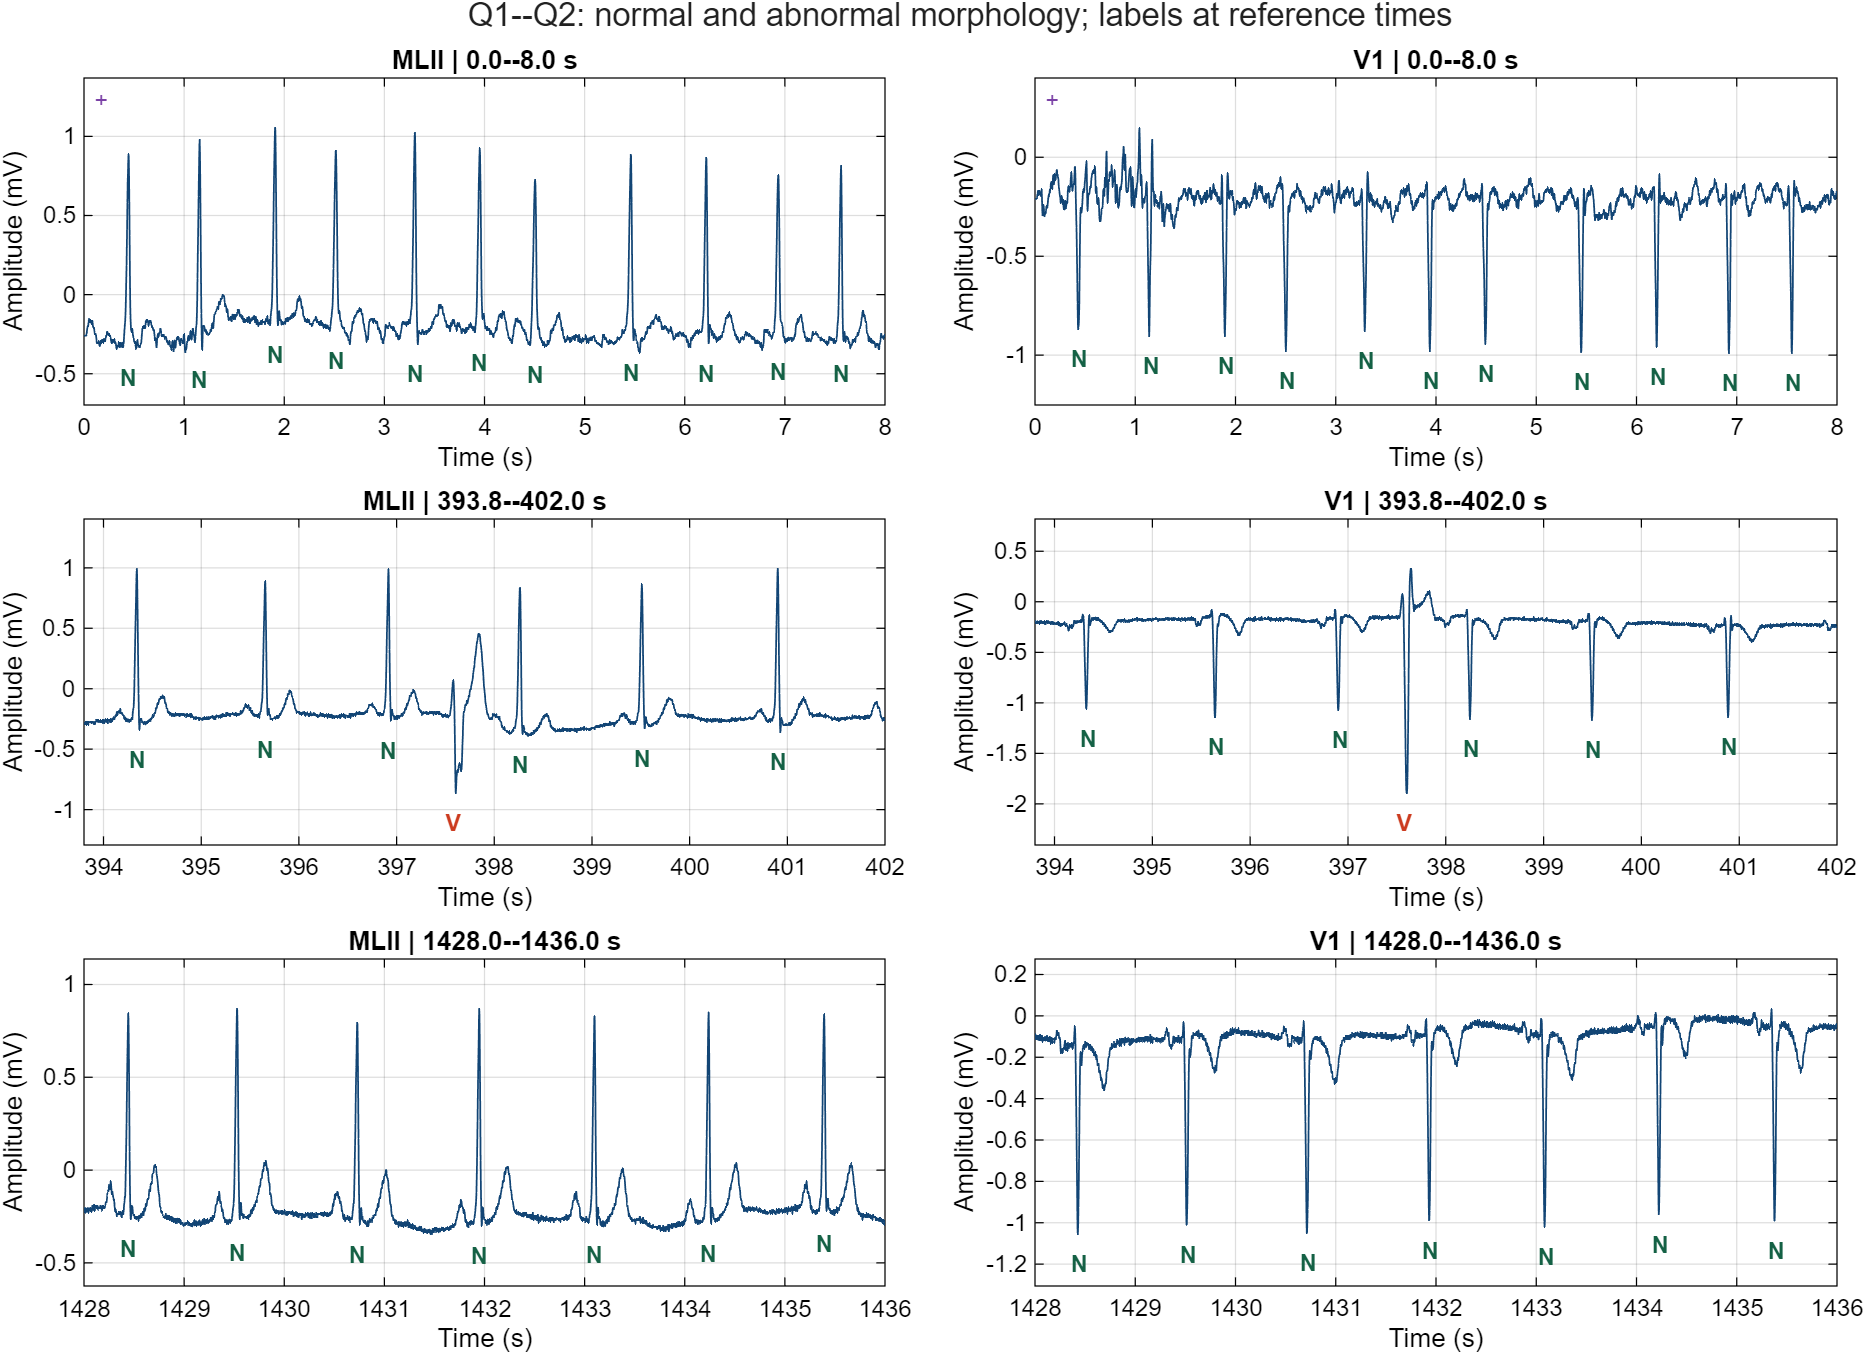
\includegraphics[width=\textwidth]{fig13_ecg_segments_with_labels.png}
\caption{Readable segments of the two leads at three different times, with the reference beat labels shown.}
\label{fig:ecgseg}
\end{figure}

For two different beats, an N sample at 1430.725~s and a V sample at 397.578~s were chosen. In Figure~\ref{fig:pqrst}, the distinguishable waves are marked for instructional purposes. The small q/s peaks are not definite in some leads; the absence of a distinguishable component must not be filled in with an artificial marker. In the ventricular sample, an independent P wave is not clear and Q has not been determined separately. The time markers are not valid clinical boundaries for measuring PR or QT.

\begin{figure}[H]
\centering
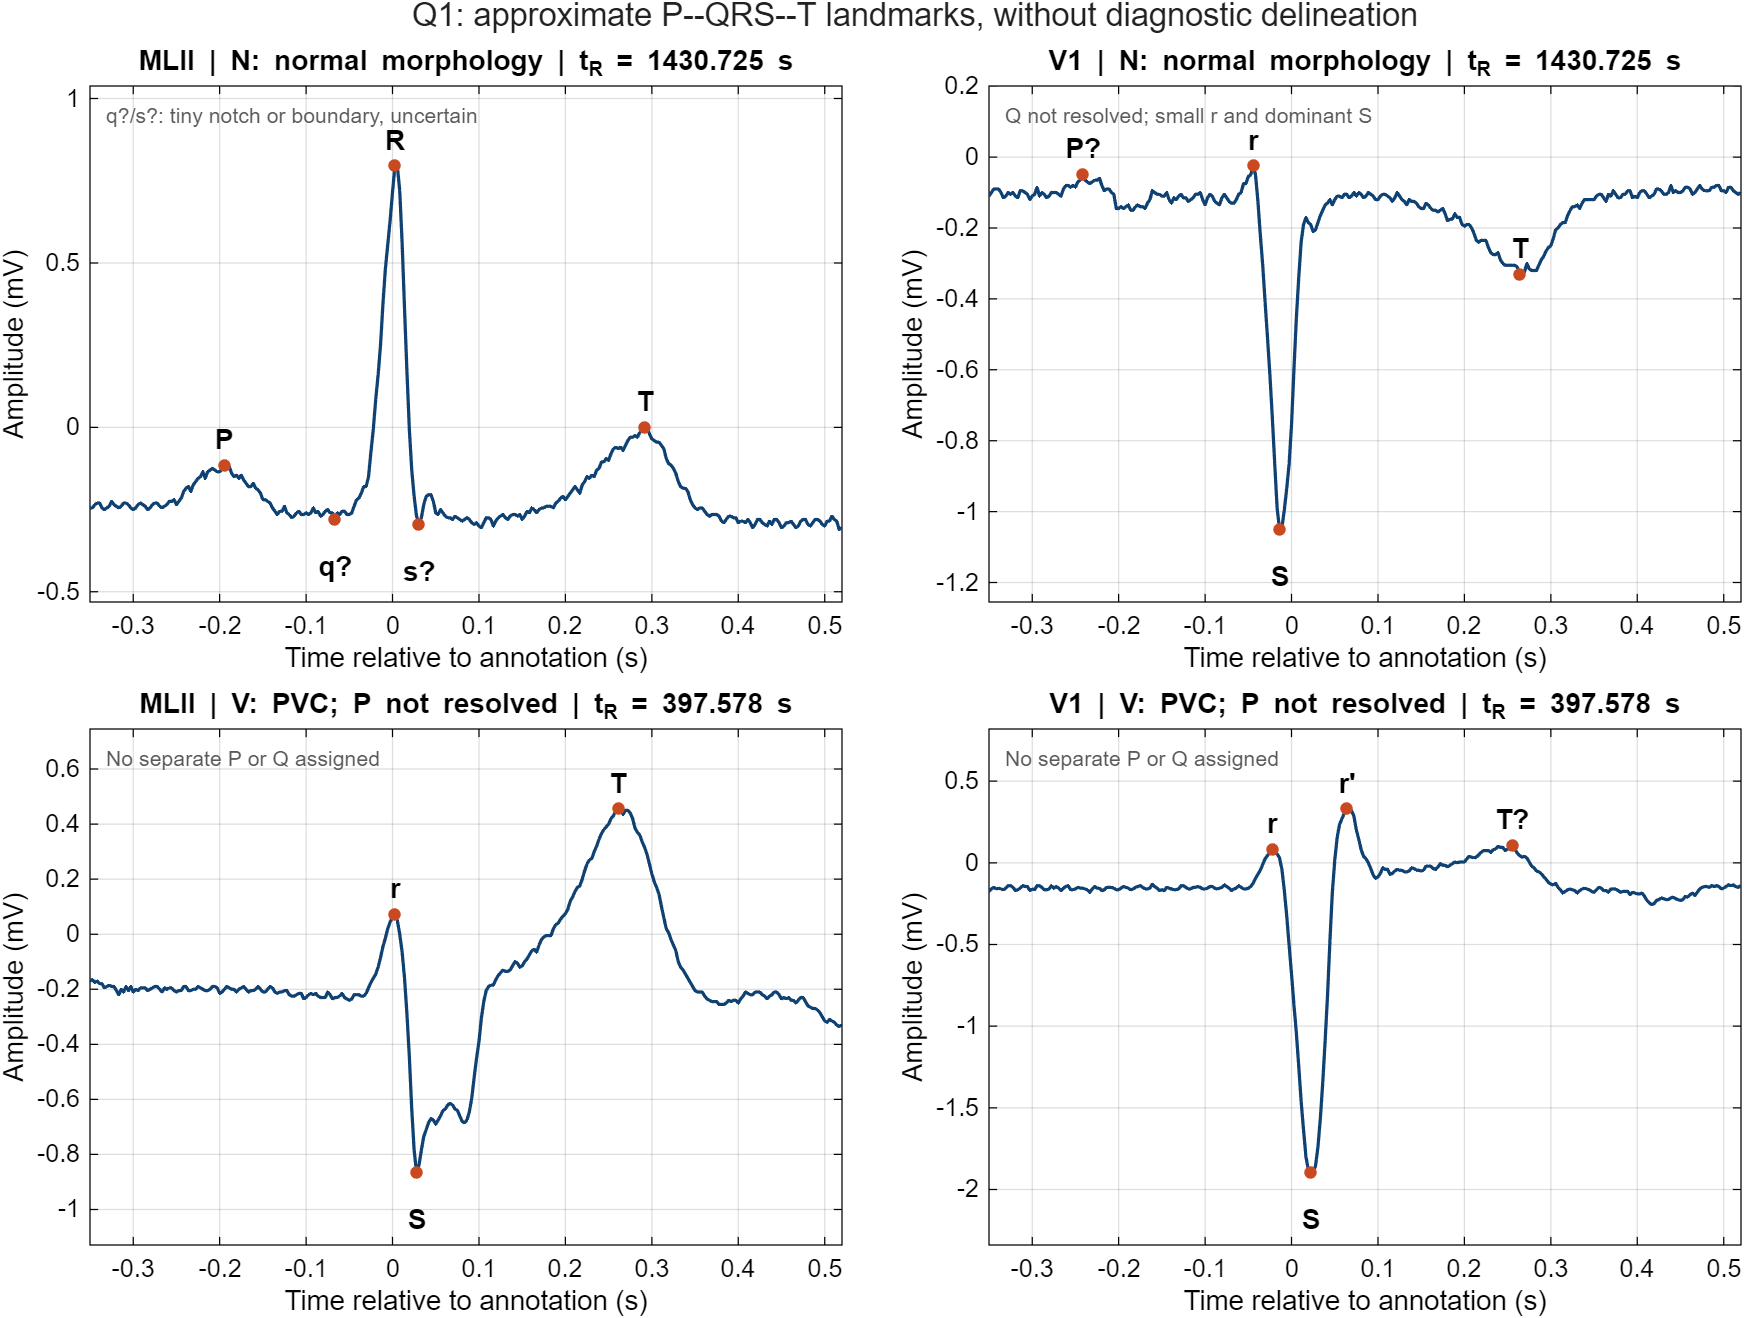
\includegraphics[width=\textwidth]{fig14_ecg_pqrst_landmarks.png}
\caption{Approximate marking of the distinguishable waves in two different beats and two leads.}
\label{fig:pqrst}
\end{figure}

The P wave is atrial activity, the QRS complex is ventricular depolarization, and the T wave is ventricular repolarization. Not all beats necessarily show all five letters as separate, clear peaks or troughs. In addition, the reference time of the database label is the characteristic time of the complex; in the second lead it may not lie exactly on the positive peak of R.

\subsection{Question 2: Interpreting Labels and Labeling All Beats}
\begin{taskbox}
The occurrence time of the R wave is given in the vector \texttt{ATRTIMED} and the type (abnormality) of the beat in the vector \texttt{ANNOTD}. The number 1 in \texttt{ANNOTD} indicates a normal beat, and every other number indicates a type of abnormality. The abnormality corresponding to each number is described in the file \texttt{ANNOTATIONS.pdf}. For the signal of each channel, write the abnormality type of each beat below it (at the time of the R peak). You can use the \texttt{text} command.
\end{taskbox}

The vectors \texttt{ATRTIMED} and \texttt{ANNOTD} give the event time and the event code, respectively. To convert time to a MATLAB index, \texttt{round(t*fs)+1} was used. The exact definition of the codes was taken from the accompanying file \texttt{ANNOTATIONS.pdf} and from the official WFDB reference. Contrary to the simplification in the exercise statement, a number other than one is not always an abnormal beat: codes 14, 28 and 37 mark a signal quality change, a rhythm change and a non-conducted atrial wave, respectively.

\begin{center}
\begin{tabularx}{\textwidth}{@{}cc>{\raggedright\arraybackslash}Xcc@{}}
\toprule
\textbf{Code} & \textbf{Symbol} & \textbf{Meaning of the event} & \textbf{Count} & \textbf{Ventricular complex}\\
\midrule
1  & N & Beat with the usual shape & 1625 & Yes\\
4  & a & Aberrated atrial premature beat & 97 & Yes\\
5  & V & Premature ventricular beat & 198 & Yes\\
6  & F & Fusion of ventricular and normal beat & 2 & Yes\\
7  & J & Premature junctional beat & 1 & Yes\\
8  & A & Premature atrial beat & 30 & Yes\\
11 & j & Junctional escape beat & 10 & Yes\\
14 & $\sim$ & Signal quality change & 4 & No\\
28 & + & Rhythm change & 35 & No\\
37 & x & Non-conducted premature atrial wave & 37 & No\\
\bottomrule
\end{tabularx}
\end{center}

In total there are 2039 events, but the number of actual ventricular complexes is 1963: 1625 N beats and 338 beats with a non-N shape, i.e.\ about 17.22\% of the beats. The 76 remaining events were not included in the computation of the RR intervals. The mean RR interval is about 0.920~s, the median is 0.863~s, and the range is 0.336 to 3.772~s. The heart rate over the whole duration of the recording is about 65.23 beats per minute; this ratio is not the same quantity as the arithmetic-mean-based $60/\mathrm{RR}$.

All 1963 beats were labeled with their reference times in both leads in the appendix file \texttt{figures/ecg\_all\_beats\_annotated.pdf}. The appendix has 61 pages, and each page shows three ten-second cuts of both leads, so that all labels are legible. The beat symbol is placed under the complex, and a non-beat event is placed above the signal. Figure~\ref{fig:ecgseg} shows examples of the labeling in the body of the report.

\subsection{Question 3: Comparing All Beat Types and Explaining Their Mechanisms}
\begin{taskbox}
Extract one or more beats of the normal type and of each abnormality, and compare their temporal-morphological features. By searching the internet, briefly explain how each type of abnormality present in this recording arises and what its characteristics are.
\end{taskbox}

For each beat type, several aligned examples and the median pattern were plotted. To compare shapes, the baseline of each segment was shifted, but the original signal was not filtered or rewritten. To prevent a neighboring beat from entering the segment, its extent was limited to half the distance to the neighbors. Figures~\ref{fig:beats1} and~\ref{fig:beats2} show the differences between the waveforms. For J only one sample, and for F two samples, exist; from such small numbers we do not infer a stable statistical result for a population.

\begin{figure}[H]
\centering
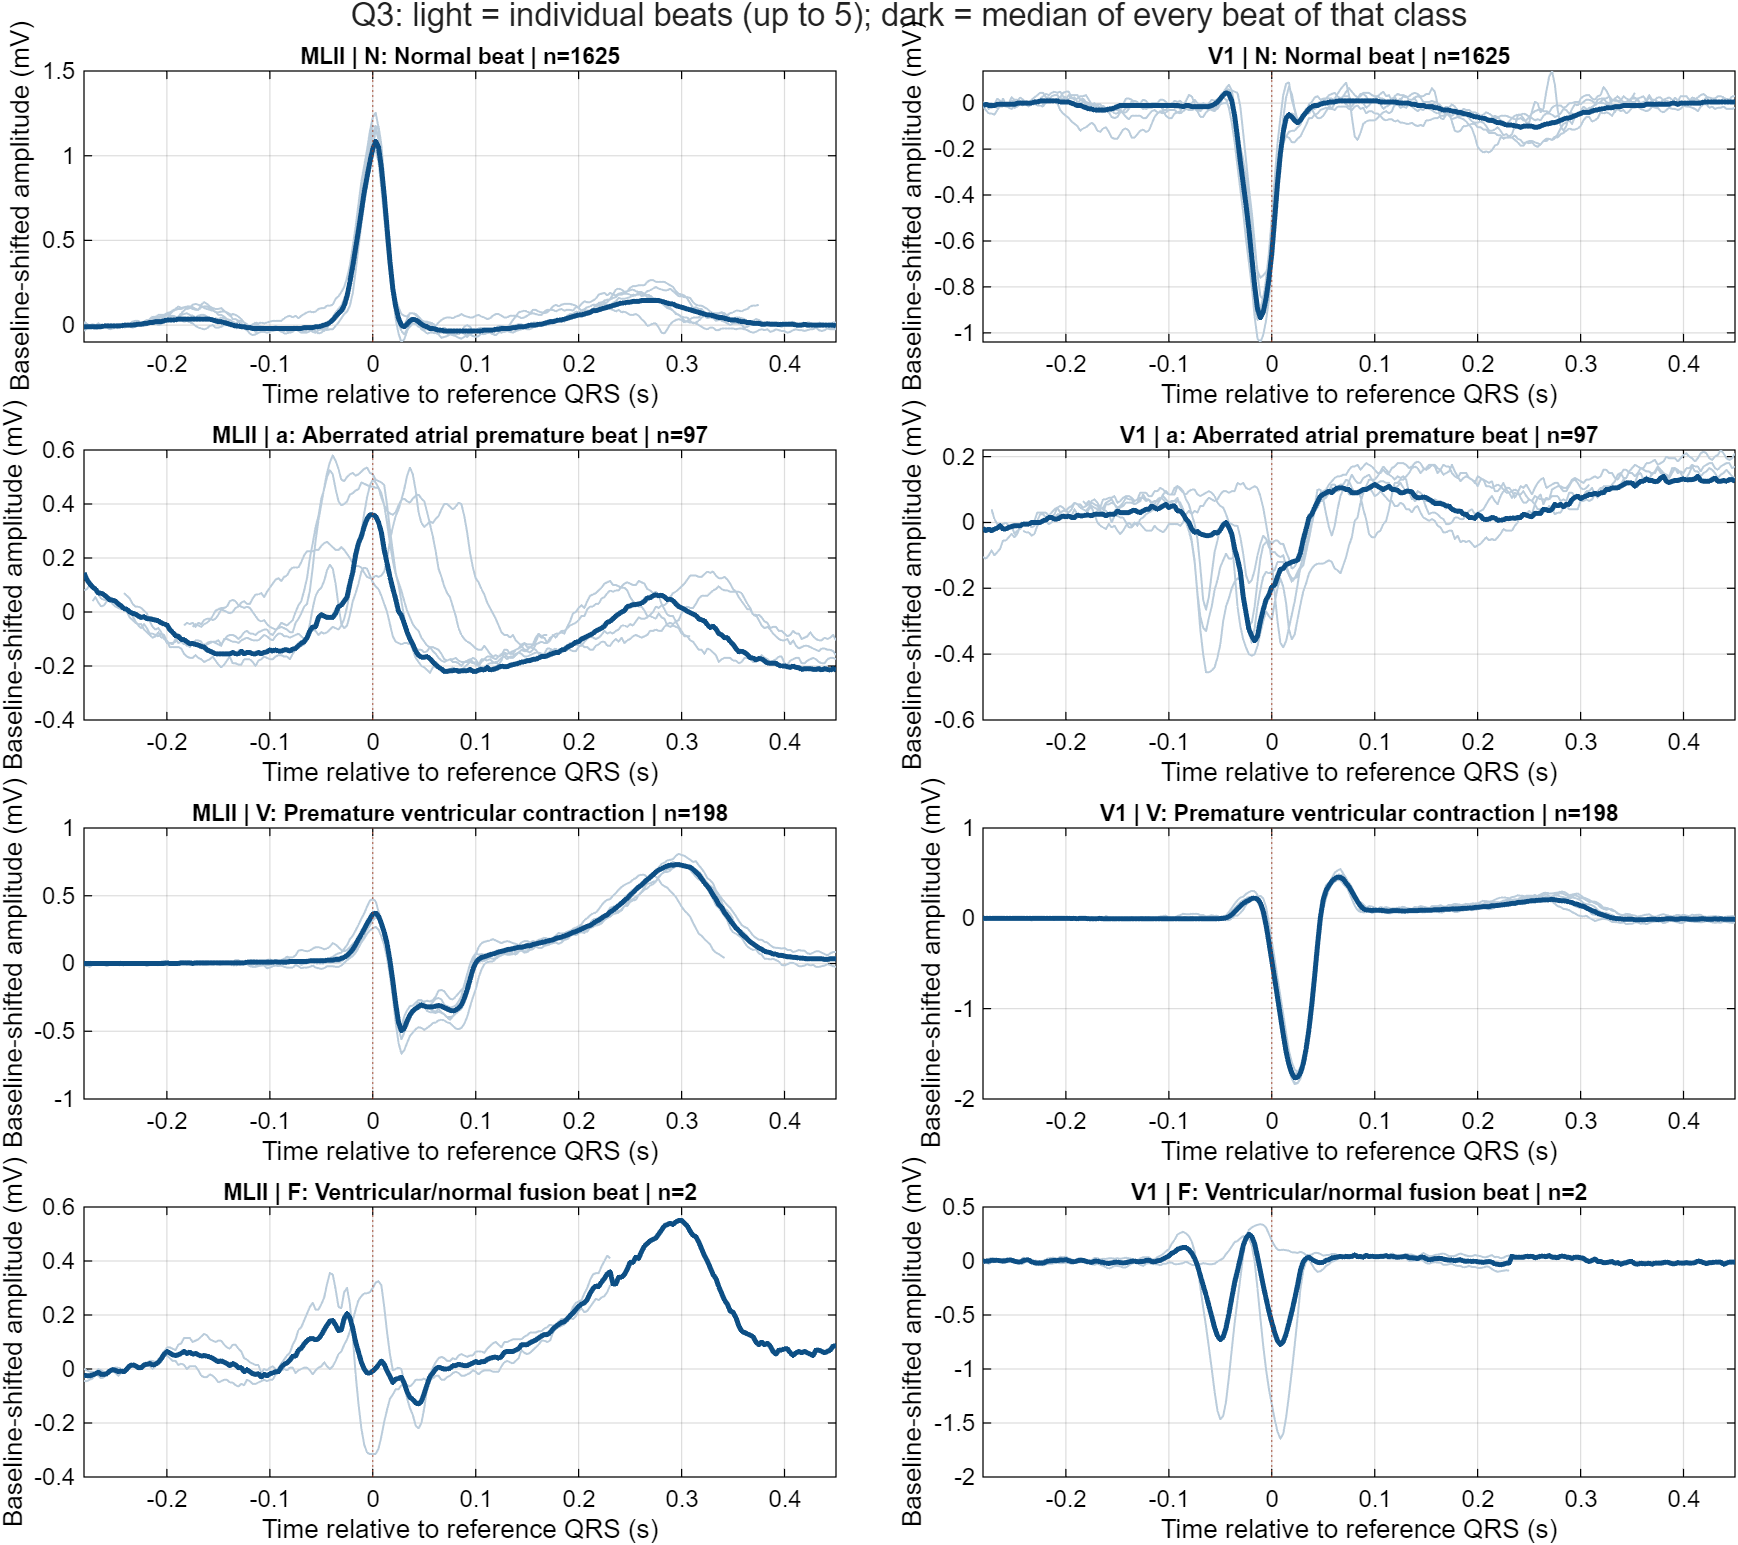
\includegraphics[width=0.95\textwidth]{fig15_beat_classes_n_a_v_f.png}
\caption{Examples and median shape of the normal beat and of the aberrant atrial, ventricular and fusion beats.}
\label{fig:beats1}
\end{figure}

\paragraph{Premature atrial beat and aberrant conduction (A and a).} In A, the stimulus starts from an atrial focus earlier than the expected beat. If ventricular conduction remains usual, the QRS can be close to that of N, and the difference is seen more in the timing and in the atrial wave. In a, the same premature atrial stimulus appears with a shape-changed QRS because of the conduction state of the bundle branches; widening of the complex alone is therefore not sufficient to call it a ventricular beat. A premature atrial stimulus may be accompanied by usual conduction, aberrant conduction or complete conduction block.

\paragraph{Premature ventricular beat (V).} In V, the ventricular stimulus does not start from the usual upstream path, and its different propagation can create a wider complex and a different return of polarity. In our data, the median shape in MLII differs from N, and the negative component and the wave after it are more prominent; the median peak-to-peak amplitude in V1 is about 2.22~mV, compared with 0.98~mV for N. Possible mechanisms of ectopic ventricular excitation include automaticity, triggered activity and re-entry; the two leads of this experiment do not determine the cellular mechanism of each event.

\paragraph{Fusion beat (F).} In F, the usual and the ectopic ventricular activation take part simultaneously in forming the complex, and the final shape can have intermediate features.

\begin{figure}[H]
\centering
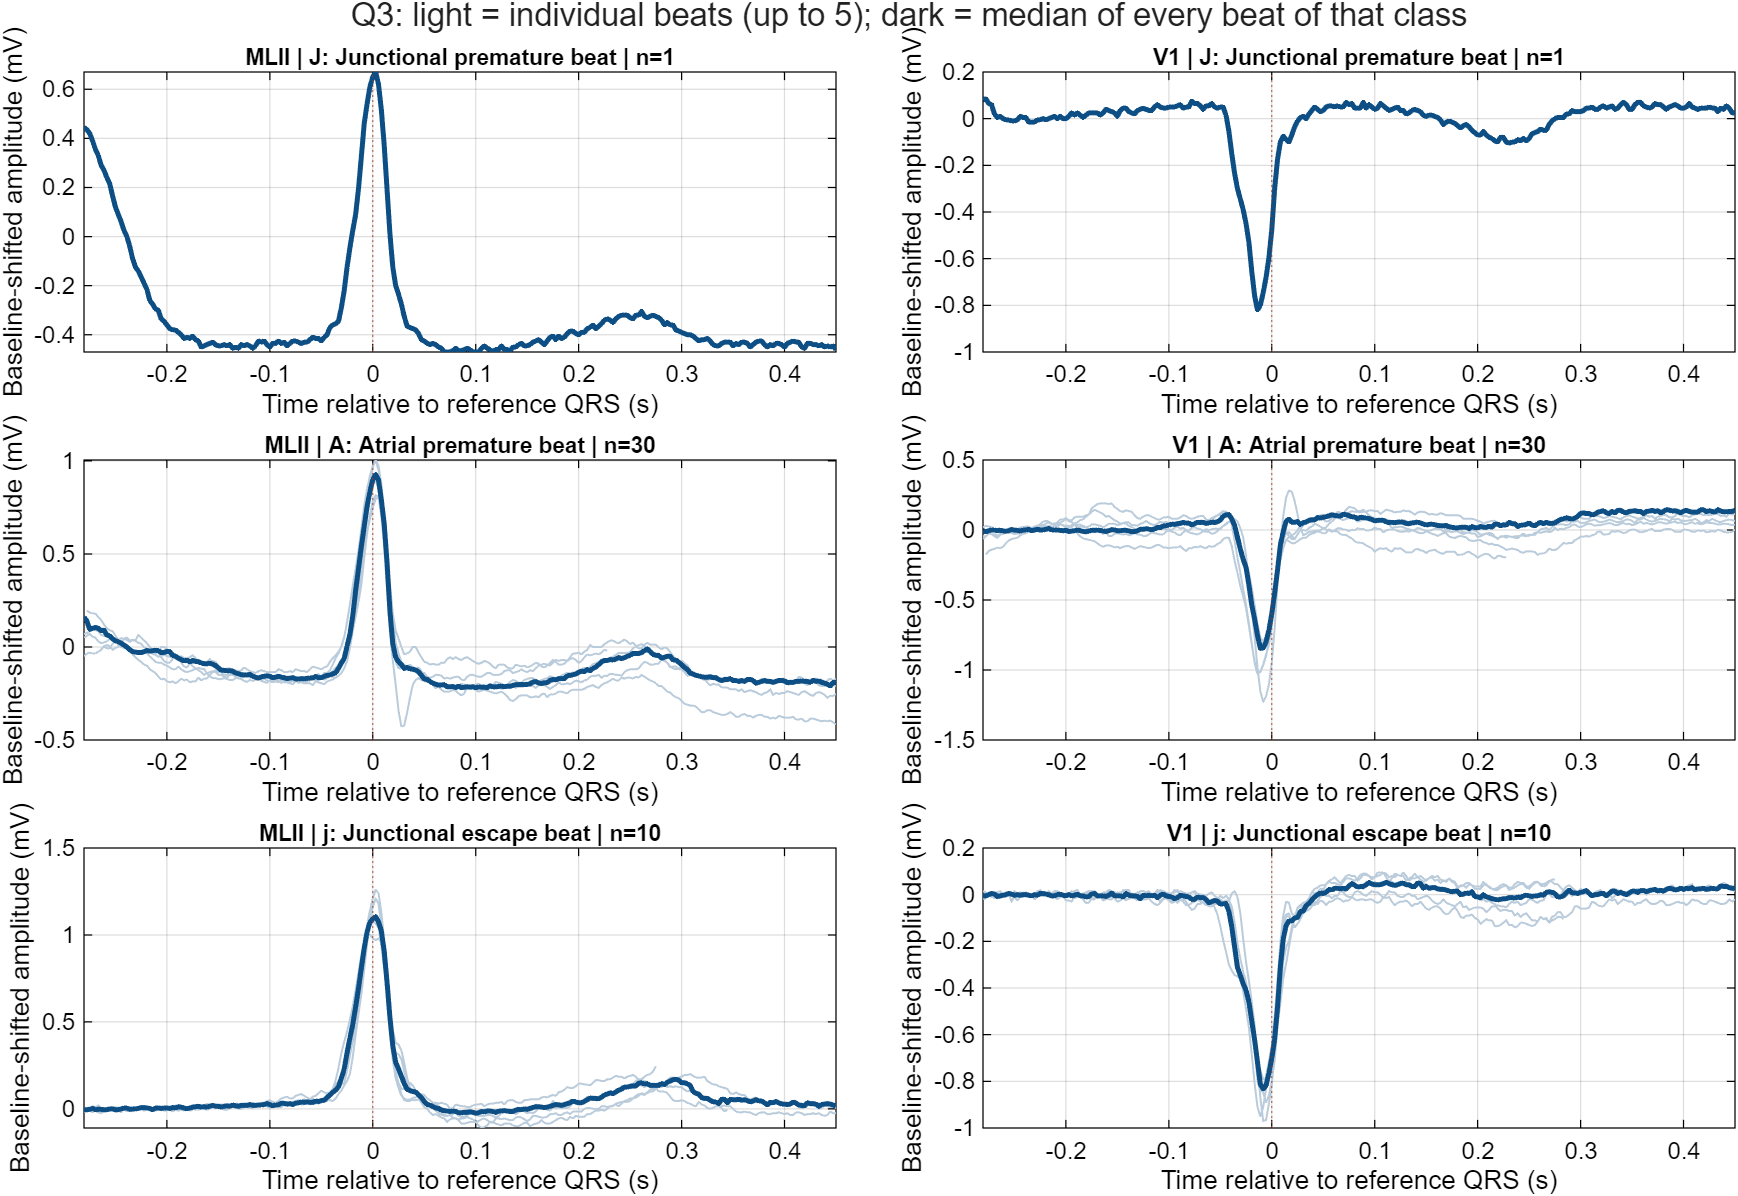
\includegraphics[width=0.95\textwidth]{fig16_beat_classes_j_A_j.png}
\caption{Examples and median shape of the junctional and atrial beats in the two leads.}
\label{fig:beats2}
\end{figure}

\paragraph{Junctional beats (J and j).} In J, the stimulus is a premature junctional one, whereas j is an escape beat after a delay in the upstream activation. Depending on the path and the conduction time, the QRS may be close to that of N, and the atrial wave may be absent, hidden or of different polarity. In the present data, the median preceding interval of J is about 0.575~s and that of j about 1.901~s; this difference is consistent with the distinction between premature and escape beats.

\paragraph{Non-conducted atrial wave (x).} The marker x belongs to a premature P wave that did not produce the next ventricular complex; for example, the stimulus can arrive while the conduction path is refractory. Figure~\ref{fig:blocked} shows an example in the context of the two leads. This event is physiologically important, but counting it as an R wave creates a false short interval in the computation of the heart rate.

\begin{figure}[H]
\centering
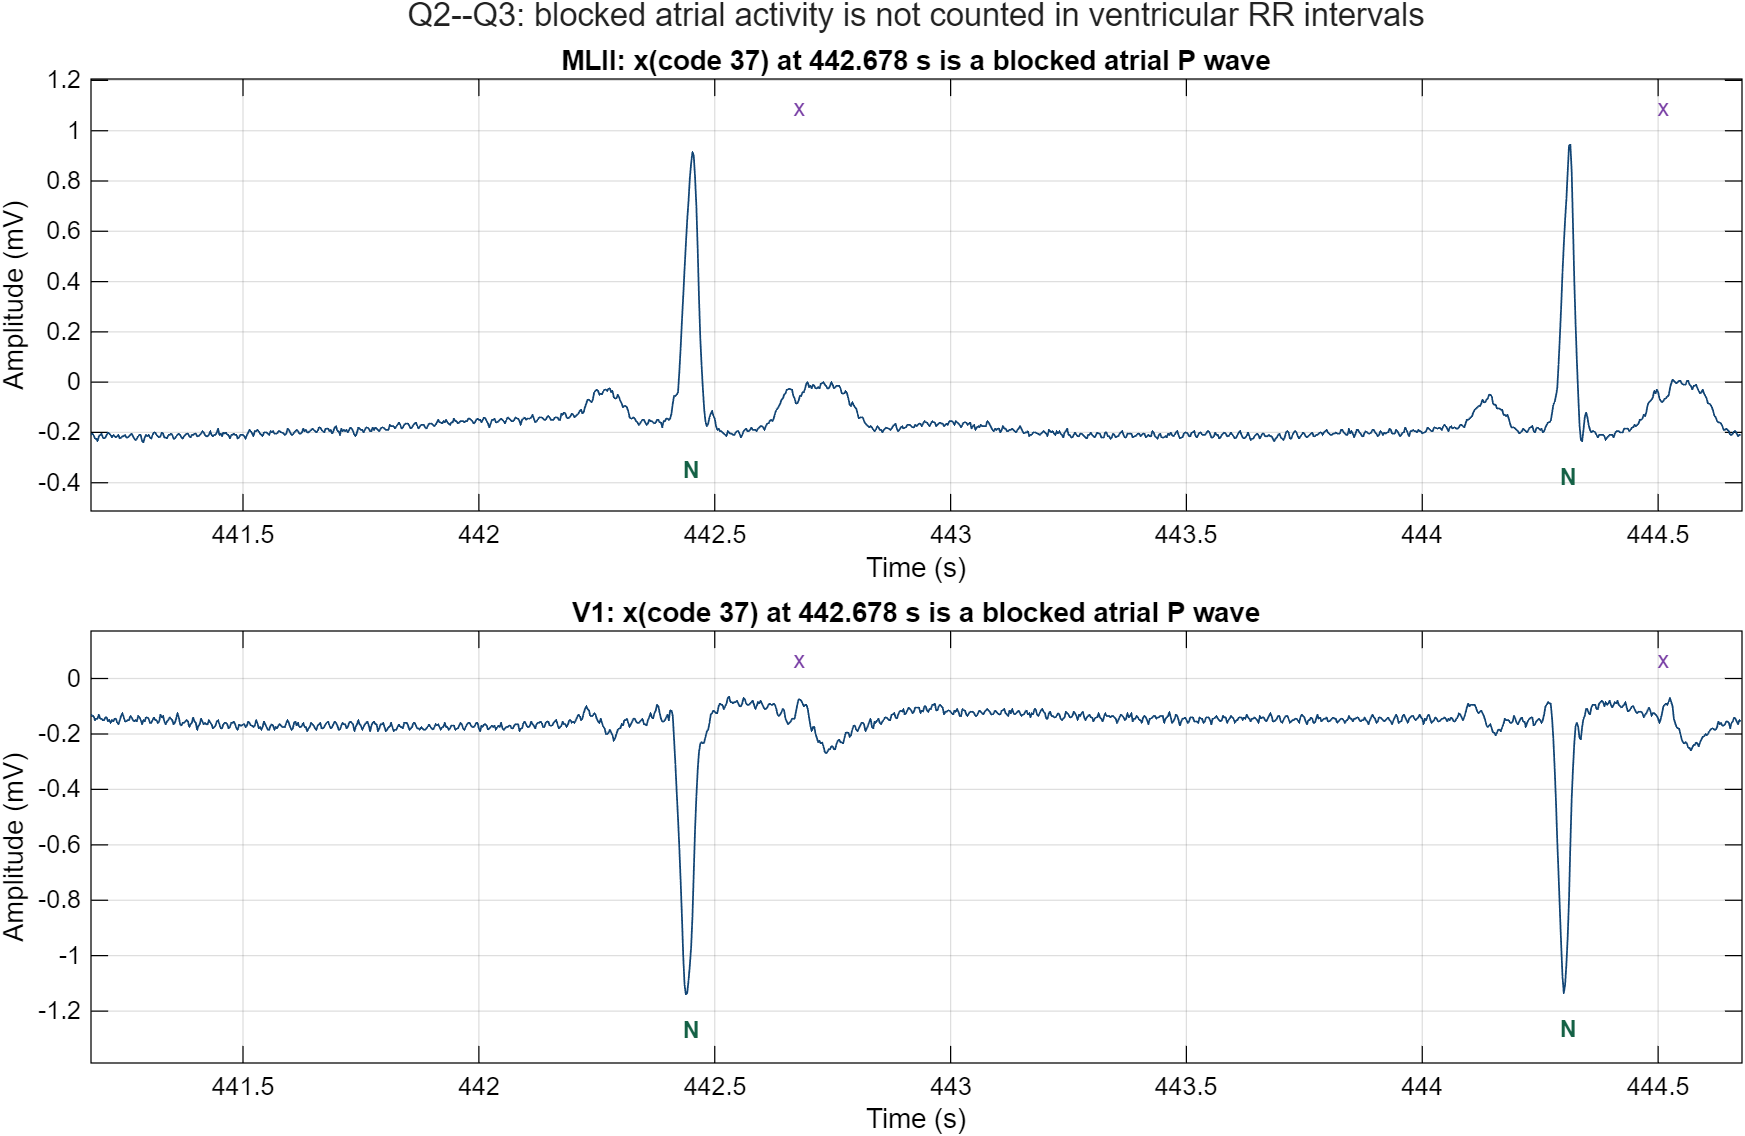
\includegraphics[width=0.95\textwidth]{fig17_blocked_atrial_wave.png}
\caption{A sample of a non-conducted atrial wave in the context of the two leads, and its separation from the ventricular beat.}
\label{fig:blocked}
\end{figure}

\subsection{Question 4: Comparing Two Segments of Three Consecutive Beats}
\begin{taskbox}
For two segments containing three consecutive beats (one segment with normal beats and one with abnormal beats), plot the frequency spectrum and the time--frequency spectrum for each channel and compare them with each other.
\end{taskbox}

One segment containing three truly consecutive beats, N--N--N, and one containing three truly consecutive beats, V--a--a, were selected; the second segment was not made by joining separate samples. The boundaries lie between the selected beat and its outer neighbor. The time of the last sample is one sampling interval shorter than the sample length of the segment.

\begin{center}
\begin{tabular}{@{}lccc@{}}
\toprule
\textbf{Segment type} & \textbf{Times of the three events (s)} & \textbf{Duration (s)} & \textbf{True Fourier resolution (Hz)}\\
\midrule
N--N--N & 1430.725 / 1431.944 / 1433.094 & 3.542 & 0.2824\\
V--a--a & 477.453 / 477.956 / 478.431 & 1.825 & 0.5479\\
\bottomrule
\end{tabular}
\end{center}

The two intervals of the normal segment are about 1.219 and 1.150~s, and those of the abnormal segment about 0.503 and 0.475~s. Besides the waveform shape, the rate of occurrence of the beats is therefore also different. Having an equal number of beats does not imply an equal temporal length or Fourier resolution.

In the spectrogram, a Hamming window of 256 samples (0.711~s), an overlap of 224 samples and \texttt{nfft=1024} were used. The time step is 0.0889~s and the spacing of the frequency grid is 0.3516~Hz. The color scale of the two conditions is common within each lead. Figures~\ref{fig:three1} and~\ref{fig:three2} place the time signal, the amplitude spectrum and the spectrogram side by side.

\begin{figure}[H]
\centering
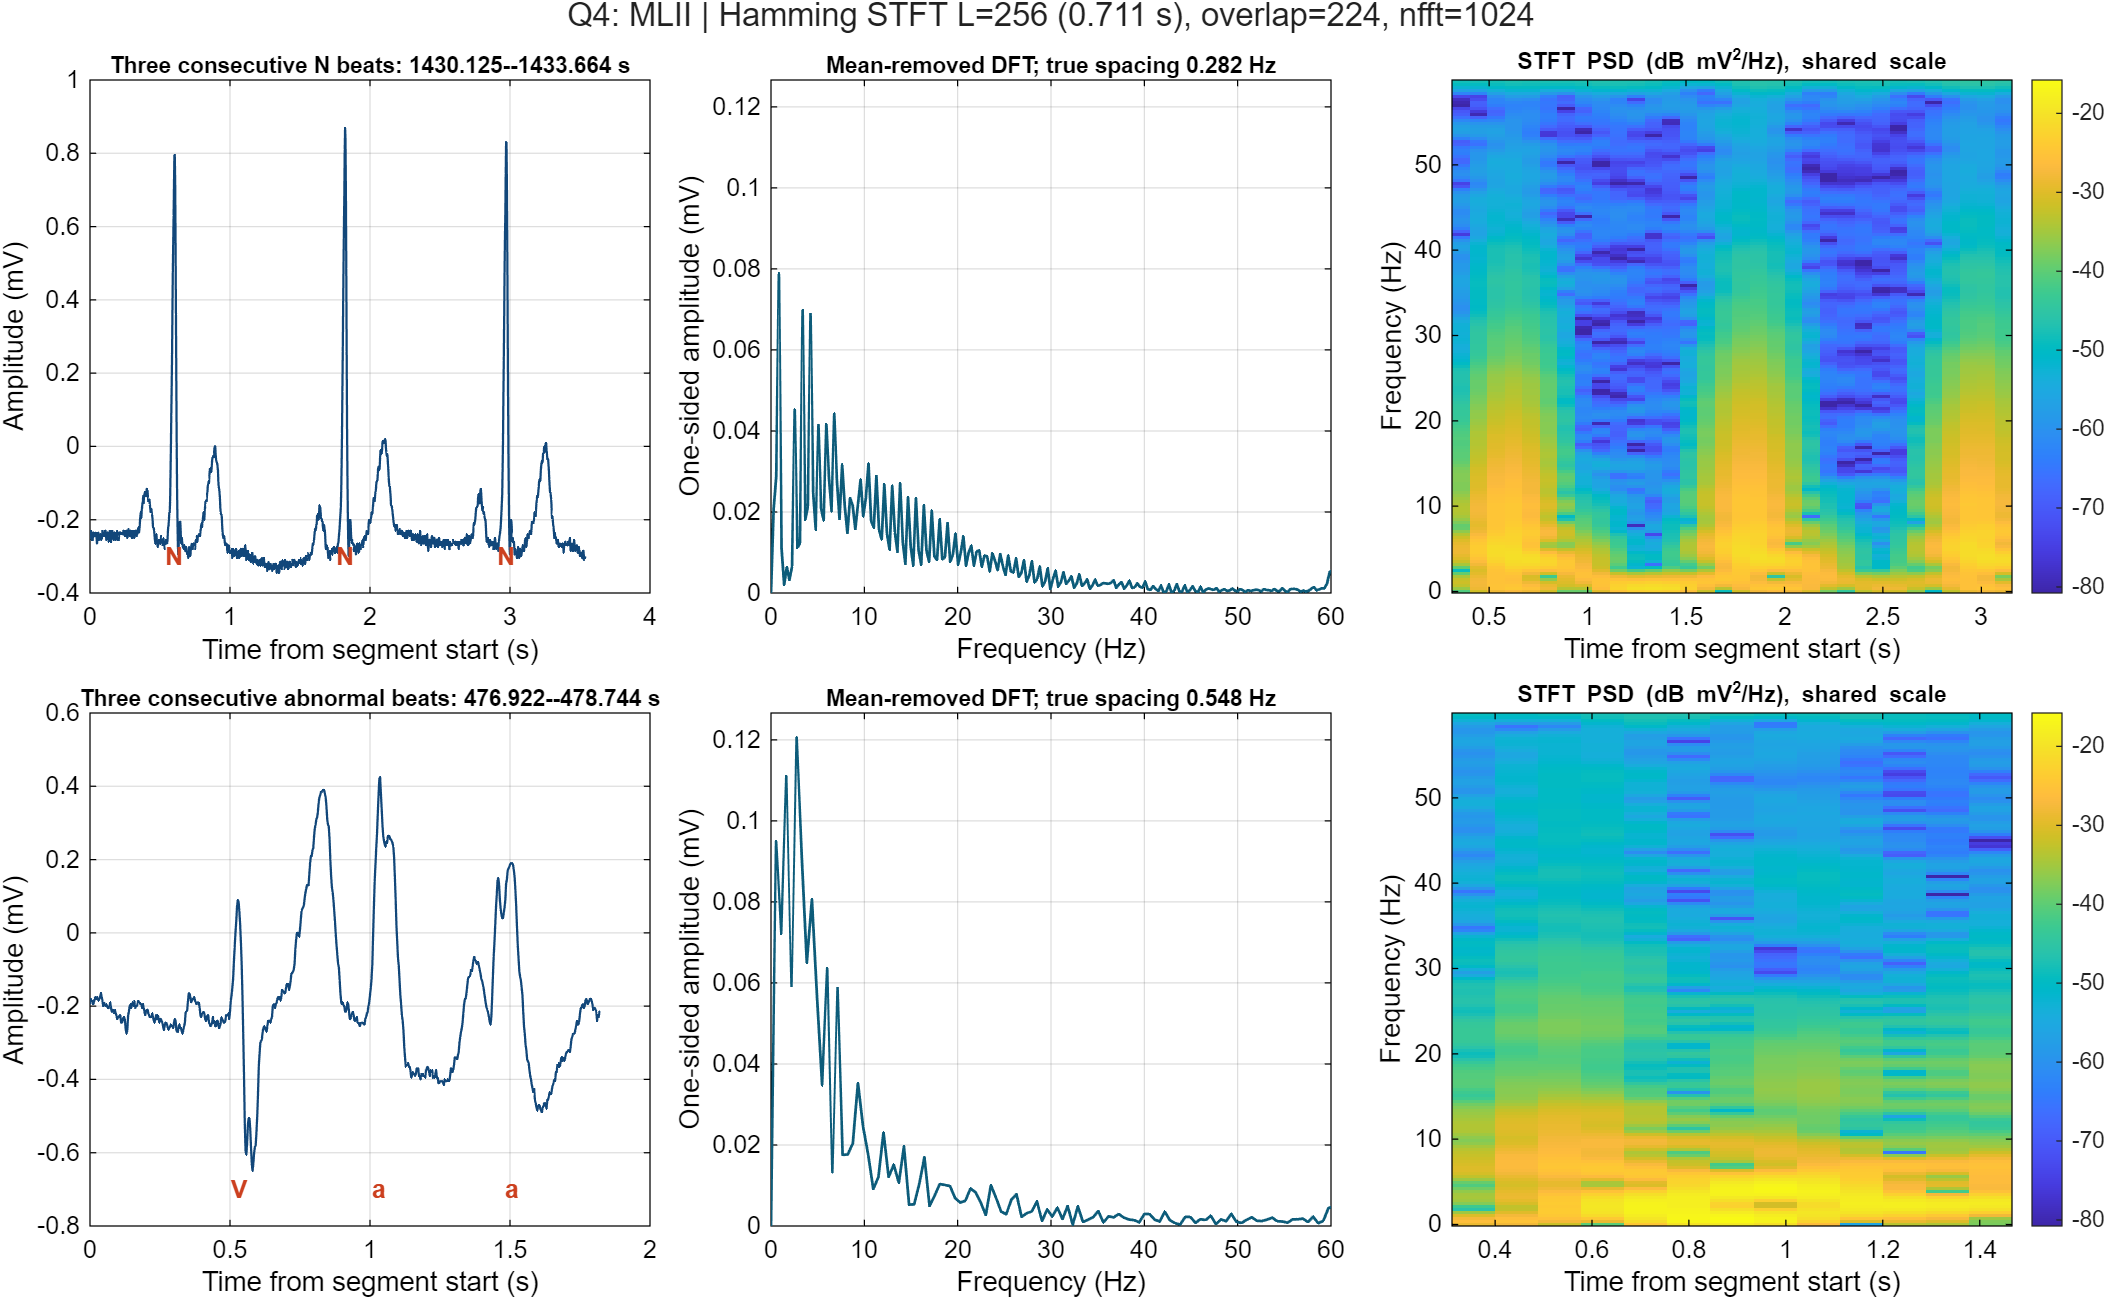
\includegraphics[width=\textwidth]{fig18_three_beats_mlii.png}
\caption{Time and spectral comparison of the two three-beat segments in the first lead.}
\label{fig:three1}
\end{figure}

In the first lead, the frequency covering 95\% of the Welch power is about 19.86~Hz for the normal segment and 10.46~Hz for the abnormal segment. Despite the shorter interval between the beats in the second segment, the power distribution of its waveform lies at lower frequencies. The rate of the beats is therefore not the same concept as the frequency of the QRS components, and it cannot be concluded that every abnormality necessarily has a higher-frequency spectrum.

\begin{figure}[H]
\centering
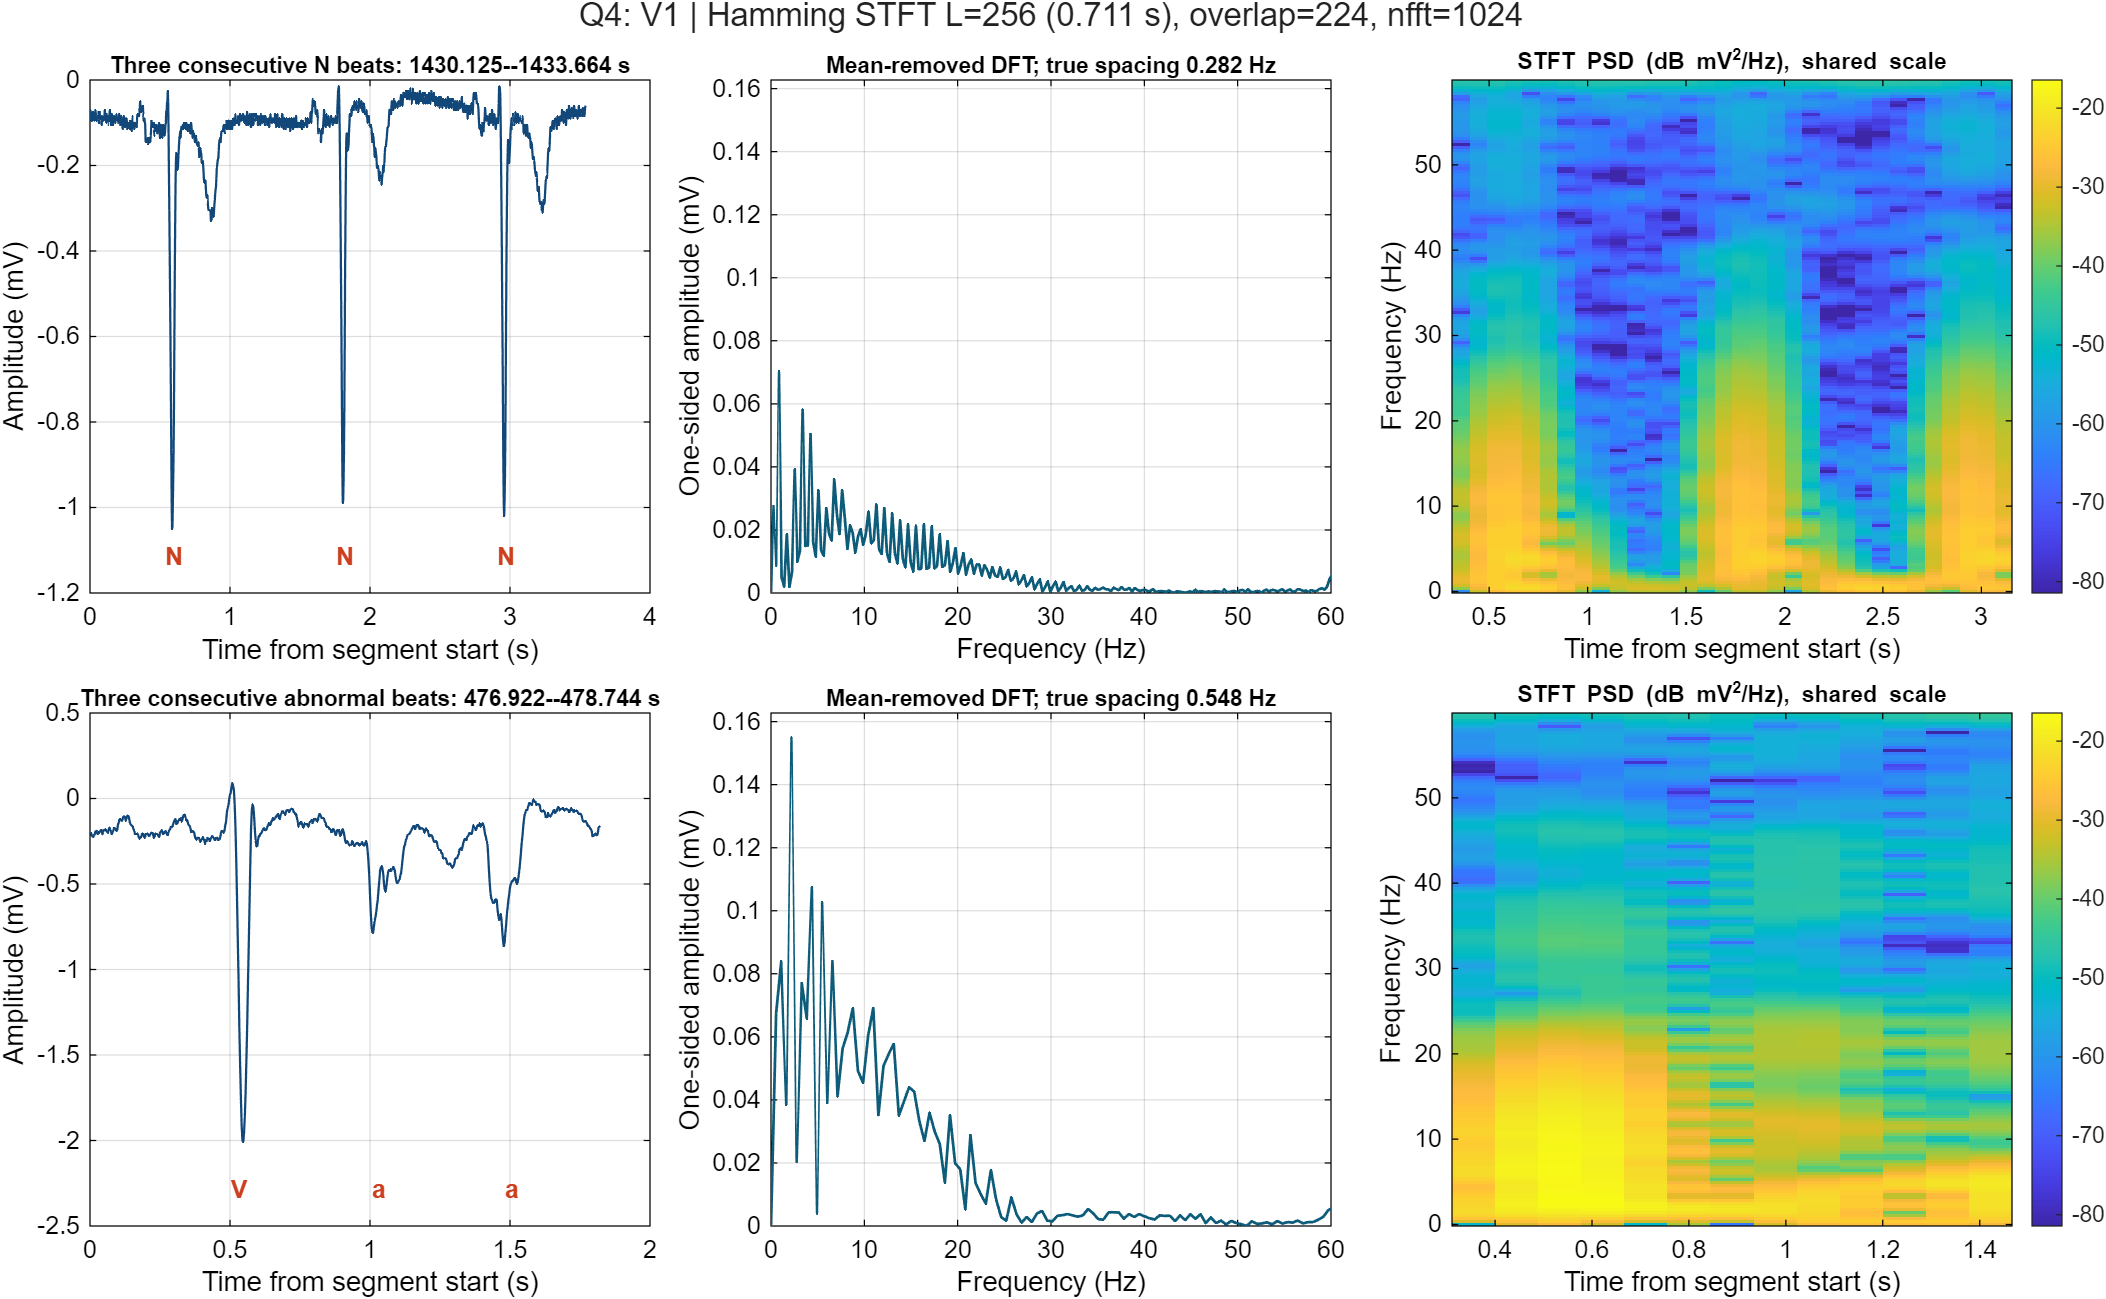
\includegraphics[width=\textwidth]{fig19_three_beats_v1.png}
\caption{Time and spectral comparison of the same two segments in the second lead.}
\label{fig:three2}
\end{figure}

In the second lead, the frequency covering 95\% of the power is about 19.60~Hz for the normal segment and 17.40~Hz for the abnormal one. The difference from the first lead results from the change in the spatial view of the cardiac activity and in the waveform shape. The spectrogram shows the temporal difference between the initial V beat and the two subsequent a beats; the overall transform sums these differences up over the whole segment. The shortness of the segments increases the fluctuation of the spectral estimate, and these results are limited to the same two segments.

\subsection{Core Implementation (ECG)}

\begin{lstlisting}[language=Matlab]
t = (0:size(Sig,1)-1)'/sfreq;     % Do not use mismatched TIME
beatCodes = [1:13 25 30 34 35 38 41];
isQRS = ismember(ANNOTD,beatCodes);
beatTimes = ATRTIMED(isQRS);
RR = diff(beatTimes);             % Excludes rhythm/quality/blocked P
\end{lstlisting}

This separation prevents the counting of non-beat events and the generation of a false heart rate. The table of the times of all events and the table of the times of the real beats are stored as two separate files in the \texttt{results} folder, and the complete code is in \texttt{code/lab1\_ecg.m}.

\section{Part 3: Eye Movement Signal (EOG)}

\begin{taskbox}[Part 3: introduction in the lab manual]
A segment of EOG recorded from two channels (left eye and right eye) is provided in the file \texttt{sig\_EOG}.
\end{taskbox}

\subsection{Question 1: Displaying and Comparing the Two Channels and the Probable Recording Arrangement}
\begin{taskbox}
Plot the signals of the two channels versus time (seconds) and compare them with each other. Based on the signal shapes, sketch the approximate placement of the recording electrodes relative to the two eyes in a figure. What information can you obtain by visually inspecting the time-domain signal?
\end{taskbox}

The EOG data have two channels, left and right, with a sampling rate of 128~Hz and a duration of 60~s. Figure~\ref{fig:eog2ch} shows the complete recording and a zoomed common interval. Slow changes, relatively constant periods and fast transitions can be seen. In part of the recording the two channels have opposite trends, but the two versions are not completely inverted copies of each other; the raw correlation is about $-0.409$.

\begin{figure}[H]
\centering
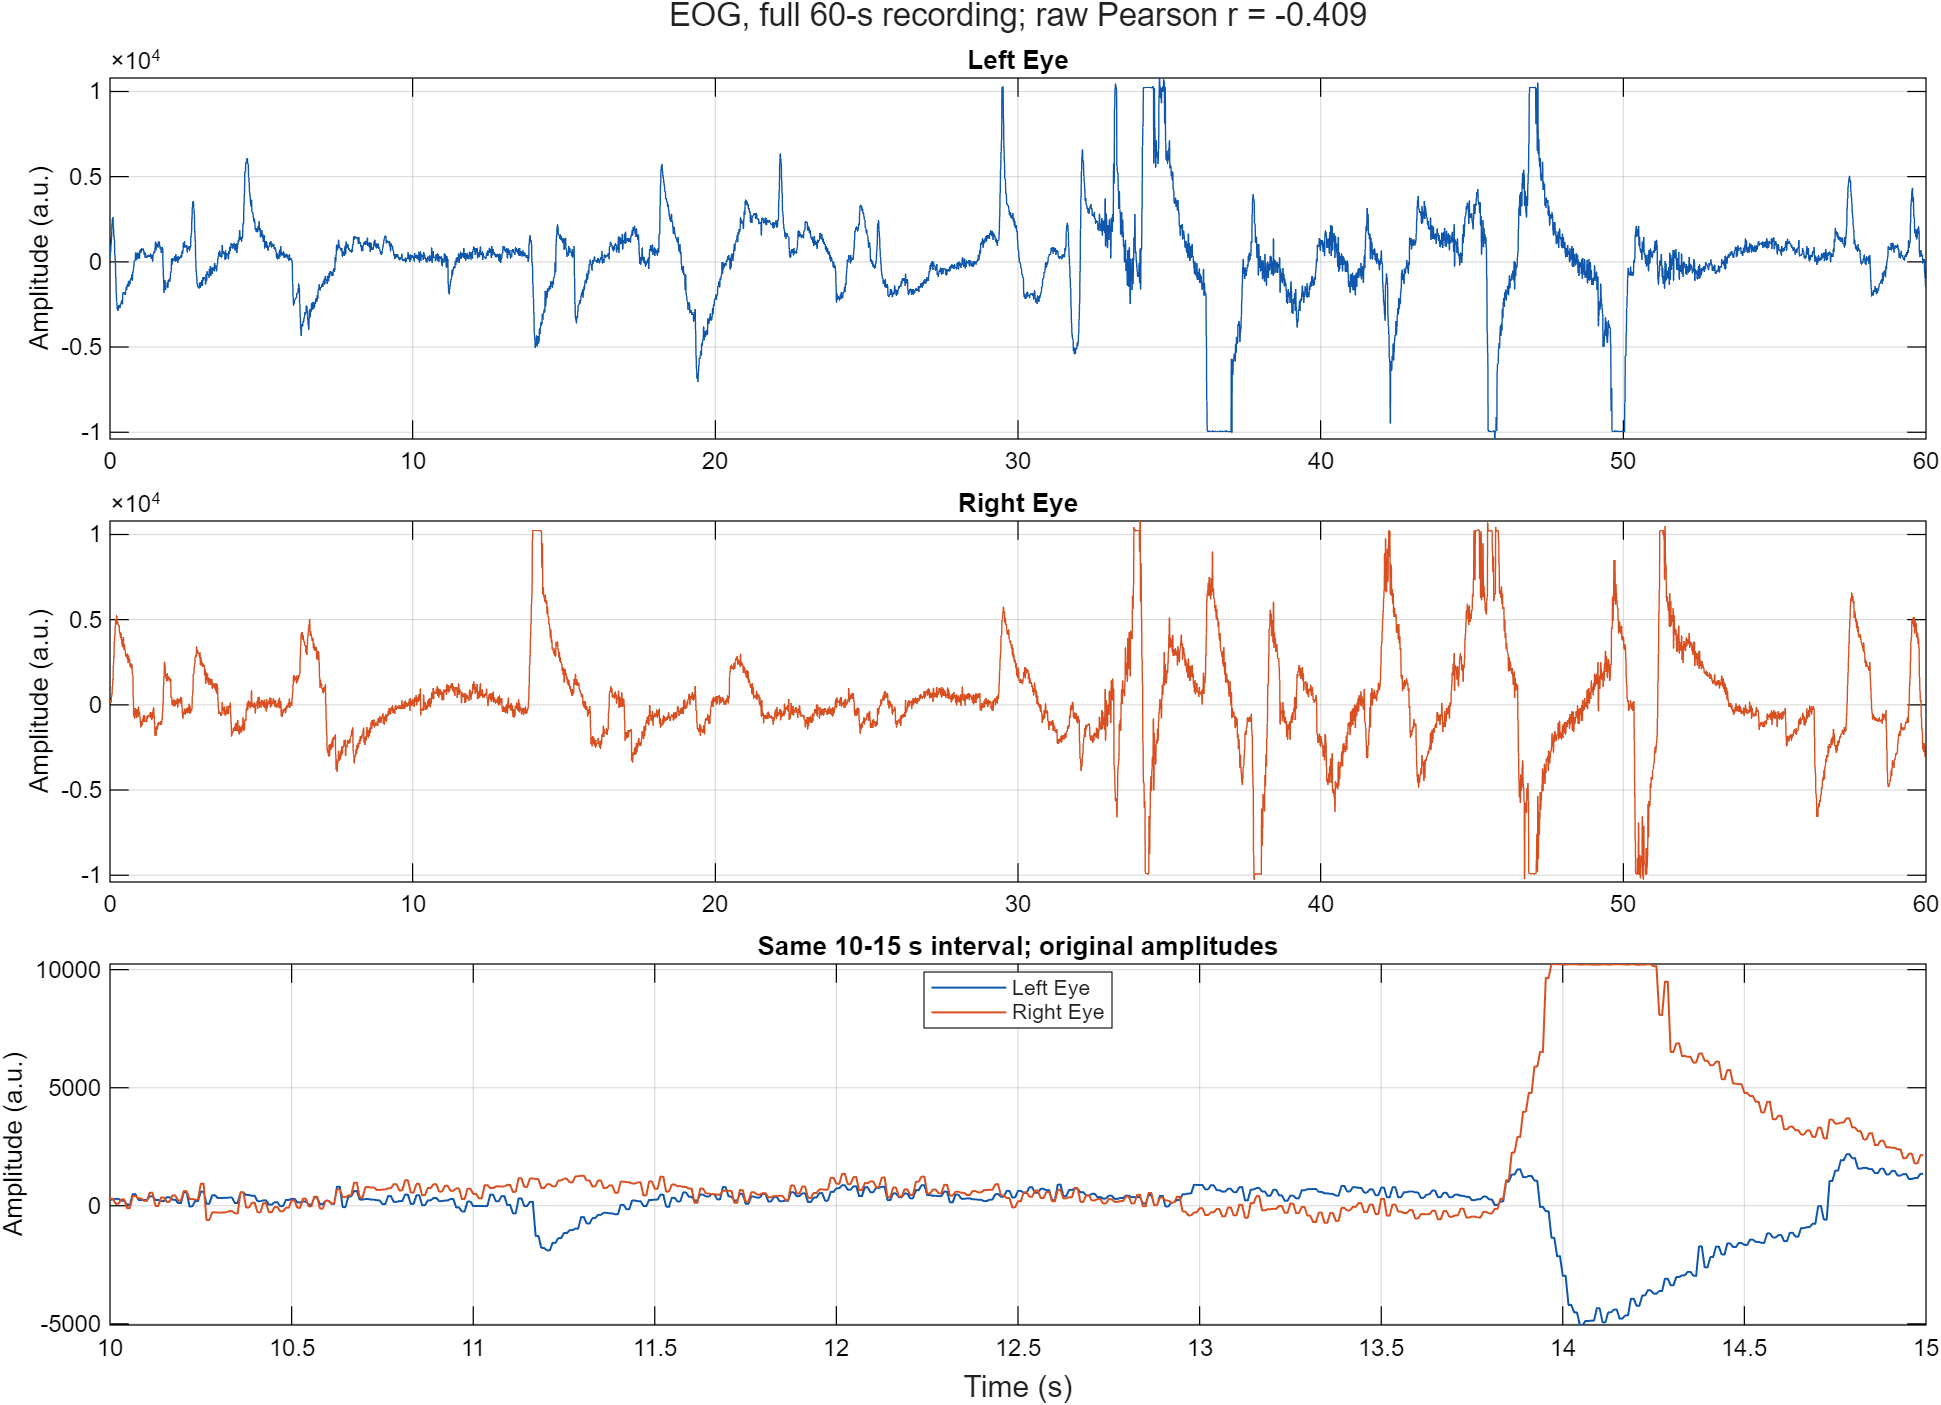
\includegraphics[width=0.95\textwidth]{fig20_eog_two_channels.png}
\caption{The two eye channels with common axes, and a zoom on the interval from ten to fifteen seconds.}
\label{fig:eog2ch}
\end{figure}

To describe the slow changes separately, a fourth-order Butterworth low-pass filter with a cutoff of 5~Hz, applied forward and backward, was used; this filter serves only for the comparison and does not replace the raw data. The correlation of the slow component is about $-0.424$, and the correlation of its derivative is about $-0.360$. Figure~\ref{fig:eogslow} emphasizes that both the trend and the timing of the transitions differ between the channels.

\begin{figure}[H]
\centering
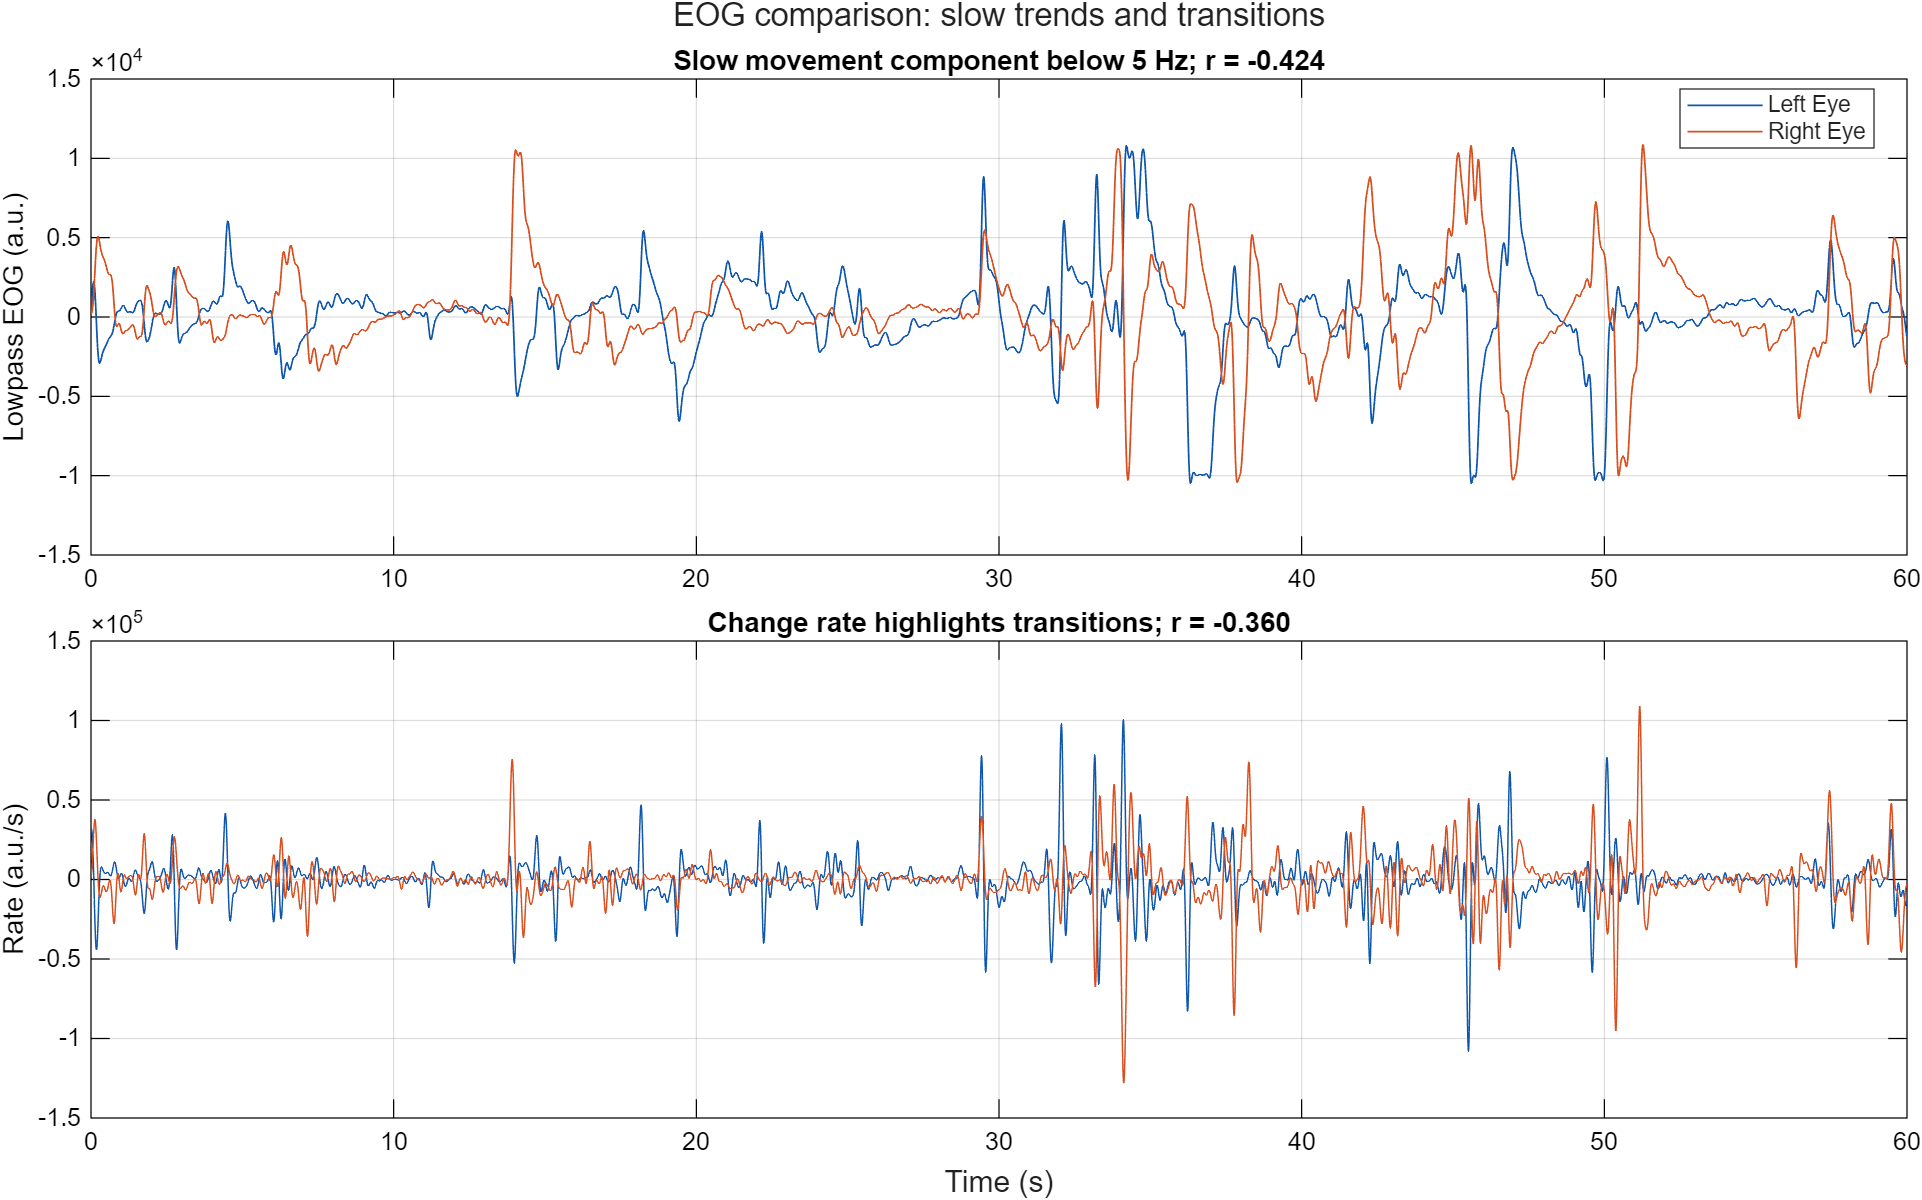
\includegraphics[width=0.95\textwidth]{fig21_eog_slow_trends_and_rate.png}
\caption{Comparison of the slow trends and their rates of change, for examining the timing of the eye transitions.}
\label{fig:eogslow}
\end{figure}

EOG recording relies on the potential difference between the cornea and the retina. An arrangement consistent with opposite changes in the two channels consists of lateral electrodes near the outer corners of the eyes and a common reference. Figure~\ref{fig:eogelec} shows this assumption from a frontal view; in this view, the left side of the person is on the right side of the image. From the two signals alone, the location of the reference, the exact locations of the electrodes or the polarity of the connection of the poles cannot be determined uniquely.

\begin{figure}[H]
\centering
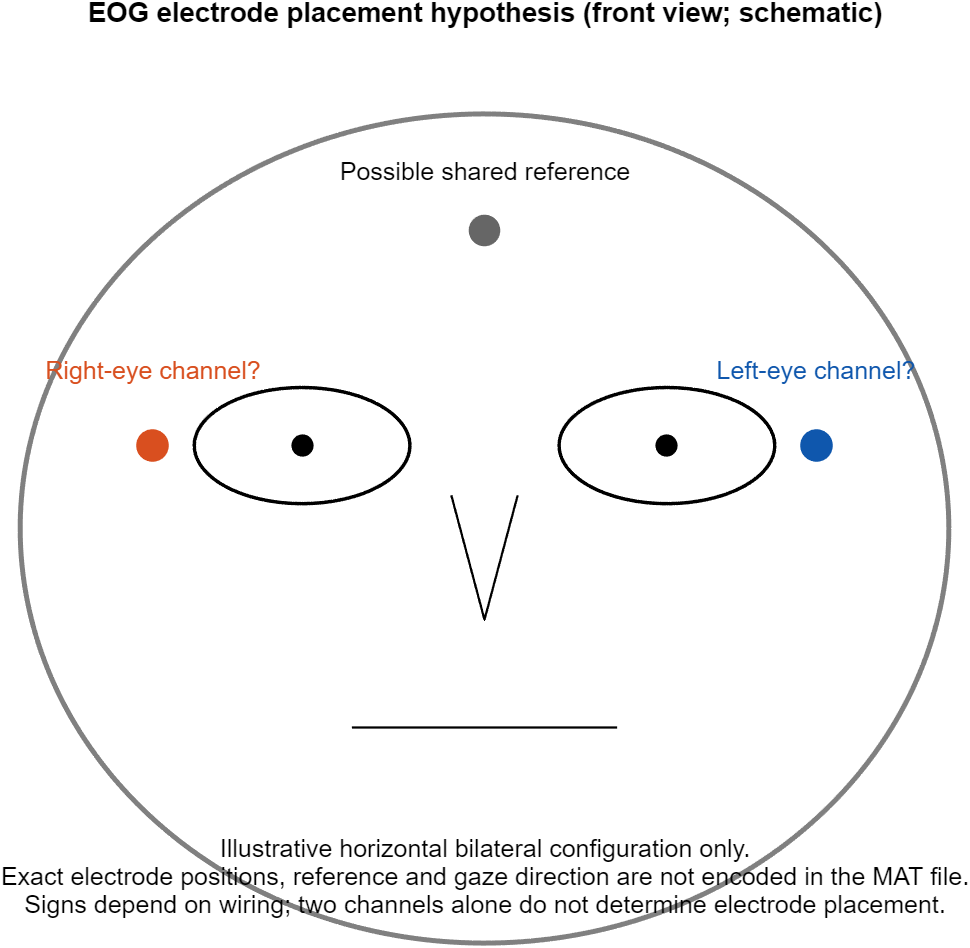
\includegraphics[width=0.6\textwidth]{fig22_eog_electrode_hypothesis.png}
\caption{A hypothetical lateral, horizontal arrangement of the electrodes for the eyes and the possible common reference.}
\label{fig:eogelec}
\end{figure}

From the time plot one can compare the timing and duration of the changes, the relative behavior of the two channels and the fast transitions. Determining the angle or the absolute direction of the gaze requires known calibration and polarity. Likewise, without a reference label, every fast transition cannot be called a blink or a saccade with certainty.

\subsection{Question 2: Frequency Spectrum and Spectrogram}
\begin{taskbox}
Plot the frequency spectrum and the time--frequency spectrum of the two channels and, based on them (and on the time-domain shape of the signals), explain the characteristics of the EOG signal.
\end{taskbox}

The one-sided Fourier transform was computed on the whole recording after removing the mean; the true spacing of its points is $1/60$~Hz. For Welch's method, a four-second Hann window, 75\% overlap and \texttt{nfft=2048} were used. According to Figure~\ref{fig:eogdft}, low-frequency components dominate. The integral of the power density below 5~Hz in both channels is about 98\% of the total Welch power.

\begin{center}
\begin{tabular}{@{}lccc@{}}
\toprule
\textbf{Channel} & \textbf{AC RMS} & \textbf{Power below 0.5~Hz (\%)} & \textbf{Power below 5~Hz (\%)}\\
\midrule
Left  & 2808.38 & 65.30 & 98.08\\
Right & 3058.52 & 58.01 & 98.00\\
\bottomrule
\end{tabular}
\end{center}

\begin{figure}[H]
\centering
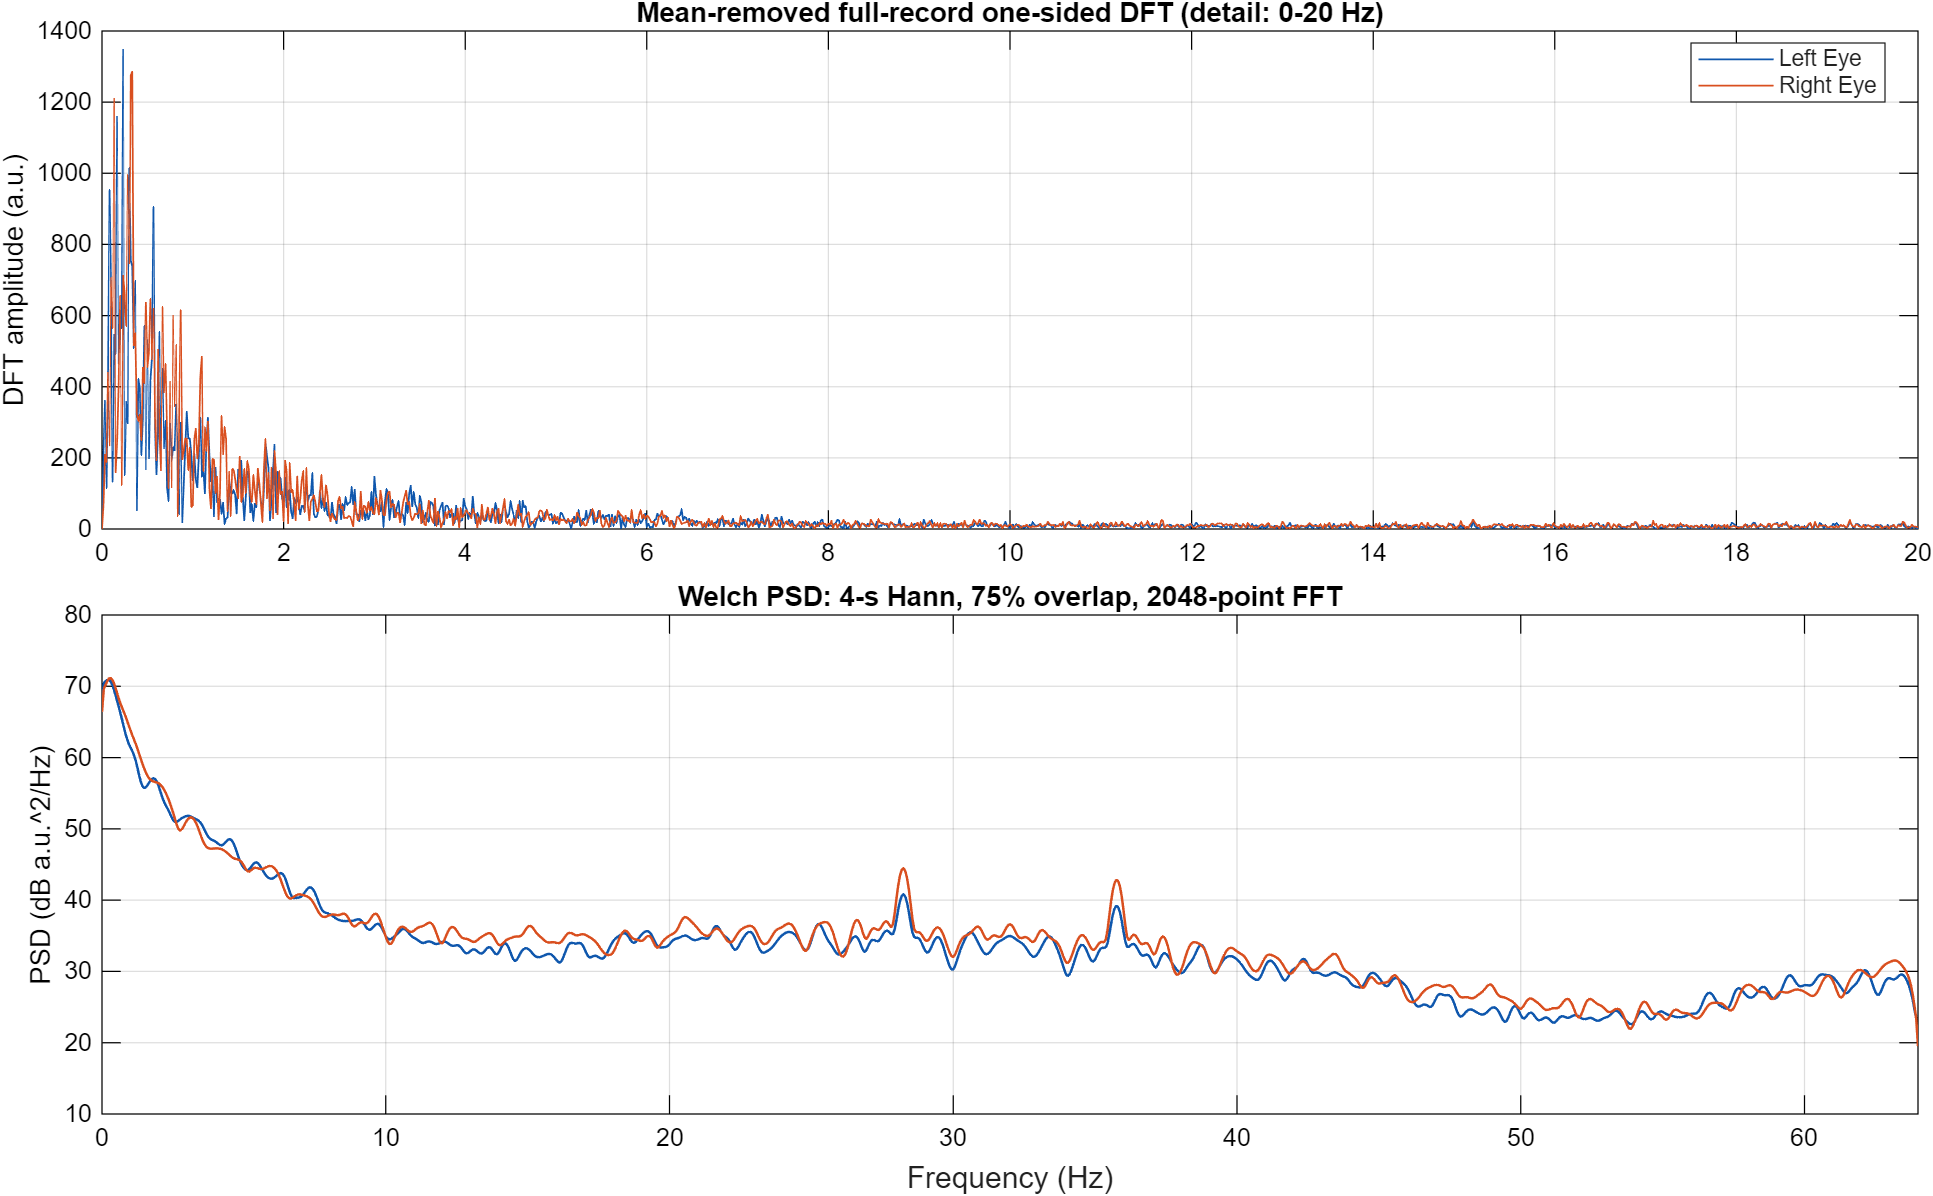
\includegraphics[width=0.95\textwidth]{fig23_eog_dft_and_psd.png}
\caption{Amplitude spectrum and power spectral density of the two eye channels, focusing on the low frequencies.}
\label{fig:eogdft}
\end{figure}

The dominance of low-frequency power is consistent with the slow changes of potential caused by eye displacement. Sharp transitions and noise can create broader energy. The RMS values of the left and right channels are close but not identical, and the peak-to-peak amplitudes of the two channels are 21168 and 21032~a.u., respectively.

For Figure~\ref{fig:eogstft}, a Hann window with a length of 256 samples, i.e.\ 2~s, an overlap of 224 samples and \texttt{nfft=1024} was used. The distribution of energy is not constant over time, and the transitions form regions of higher power at specific times. The overall spectrum shows the existence of low-frequency energy, but the spectrogram shows that this energy is not the same at all times. Faster components and noise are present alongside the dominant slow behavior.

\begin{figure}[H]
\centering
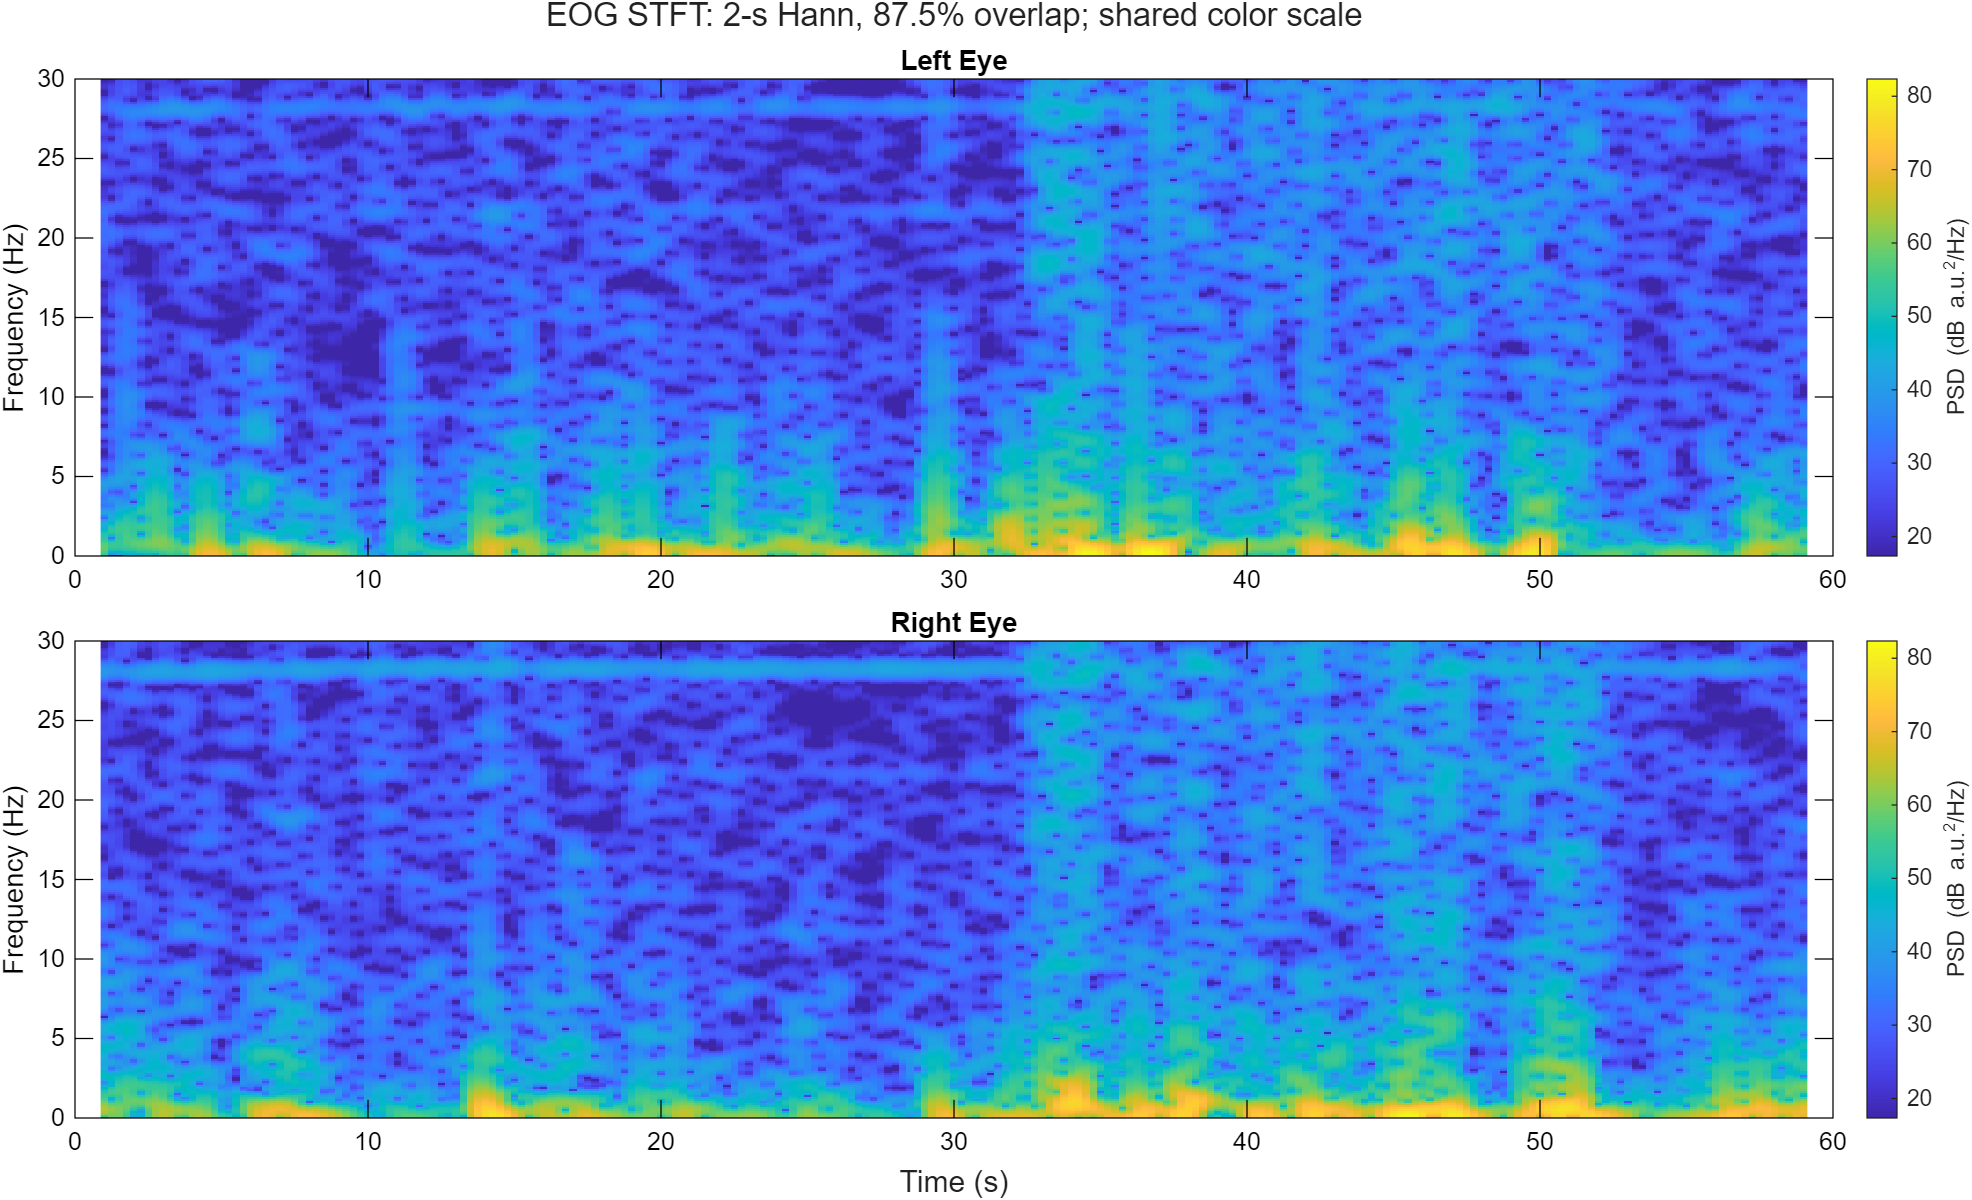
\includegraphics[width=0.95\textwidth]{fig24_eog_stft.png}
\caption{Spectrogram of the two eye channels with a common color scale, showing the temporal variations of the energy.}
\label{fig:eogstft}
\end{figure}

\subsection{Core Implementation (EOG)}

\begin{lstlisting}[language=Matlab]
t = (0:size(Sig,2)-1)/fs;
X = Sig-mean(Sig,2);
[P,f] = pwelch(X(1,:),hann(512,'periodic'),384,2048,fs);
[S,F,T,Ptf] = spectrogram(X(1,:),hann(256,'periodic'),224,1024,fs);
\end{lstlisting}

In this file the channels are rows; paying attention to this orientation prevents building an incorrect time axis or taking the Fourier transform along the channel axis. The complete implementation, together with the figure of the electrode arrangement, is in \texttt{code/lab1\_eog\_emg.m}.

\section{Part 4: Muscle Signal (EMG)}

\begin{taskbox}[Part 4: introduction in the lab manual]
Three EMG segments recorded from three subjects using needle electrodes are provided in the file \texttt{sig\_EMG.mat}. The signals were sampled at 50~kHz and the sampling frequency was then reduced to 4~kHz. One segment belongs to a healthy subject and the other two belong to two patients (Neuropathy and Myopathy). More details about the data can be found at \url{https://archive.physionet.org/physiobank/database/emgdb}.
\end{taskbox}

\subsection{Question 1: Displaying Three Subjects and Examining Waveform Shape at Several Times}
\begin{taskbox}
Plot the time-domain signal of each of the three subjects. Zoom on the horizontal axis in different parts of the signal, examine the features of each signal, and compare them with each other.
\end{taskbox}

Three segments from subjects labeled healthy, myopathy and neuropathy were analyzed. The recordings are of the needle type and, in the version of the data used in this experiment, have a sampling rate of 4000~Hz. According to the official description of the source, the needle electrode was placed in the tibialis anterior muscle, and the original recording was made during mild contraction while lifting the foot against resistance; the original rate of 50~kHz was then reduced to 4~kHz.

The lengths of the recordings are not equal: healthy 12.715~s, myopathy 27.584~s and neuropathy 36.9645~s. Figure~\ref{fig:emgfull} shows all the data with a common scale. The empty space after the end of each recording means that there is no data; it must not be interpreted as muscle silence or zero activity. In the neuropathy recording, transients of larger amplitude are prominent.

\begin{figure}[H]
\centering
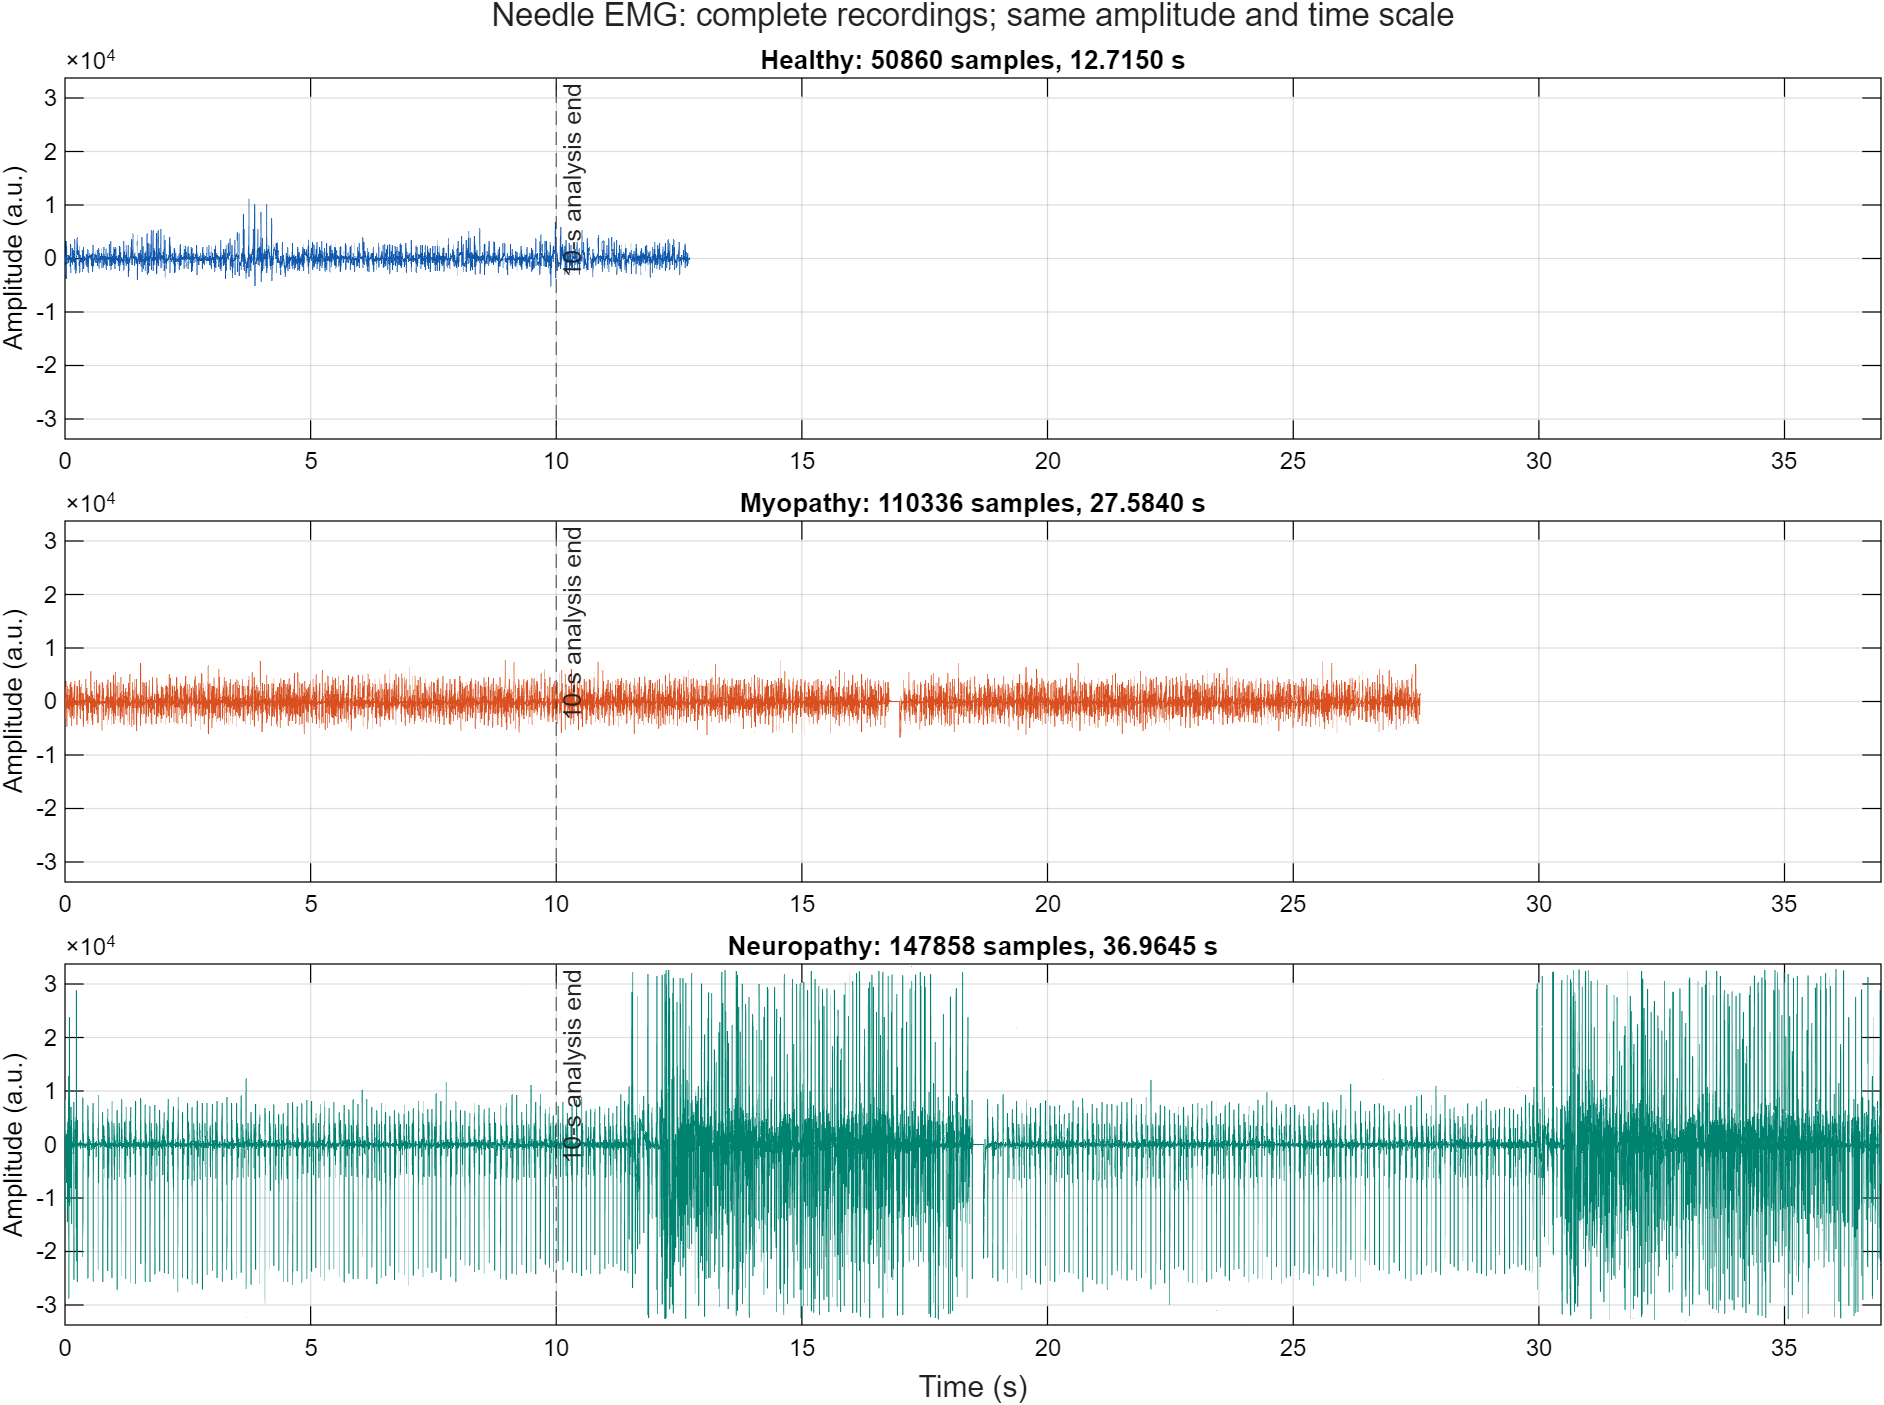
\includegraphics[width=0.95\textwidth]{fig25_emg_full_recordings.png}
\caption{Complete recordings of the three muscle samples with identical time and amplitude axes.}
\label{fig:emgfull}
\end{figure}

For the numerical and spectral comparison, only the first 10 seconds of each recording, i.e.\ 40000 common samples, were selected. Figure~\ref{fig:emg10} shows these intervals on an identical amplitude scale. The stored amplitudes were kept raw; the exercise file has no calibration. The headers of the original database give a factor of 10000~ADC/mV, but the complete equality of the versions, especially the one-sample difference in the original myopathy file, is not proved by the exercise file itself; the unit of the plots is therefore a.u.

\begin{figure}[H]
\centering
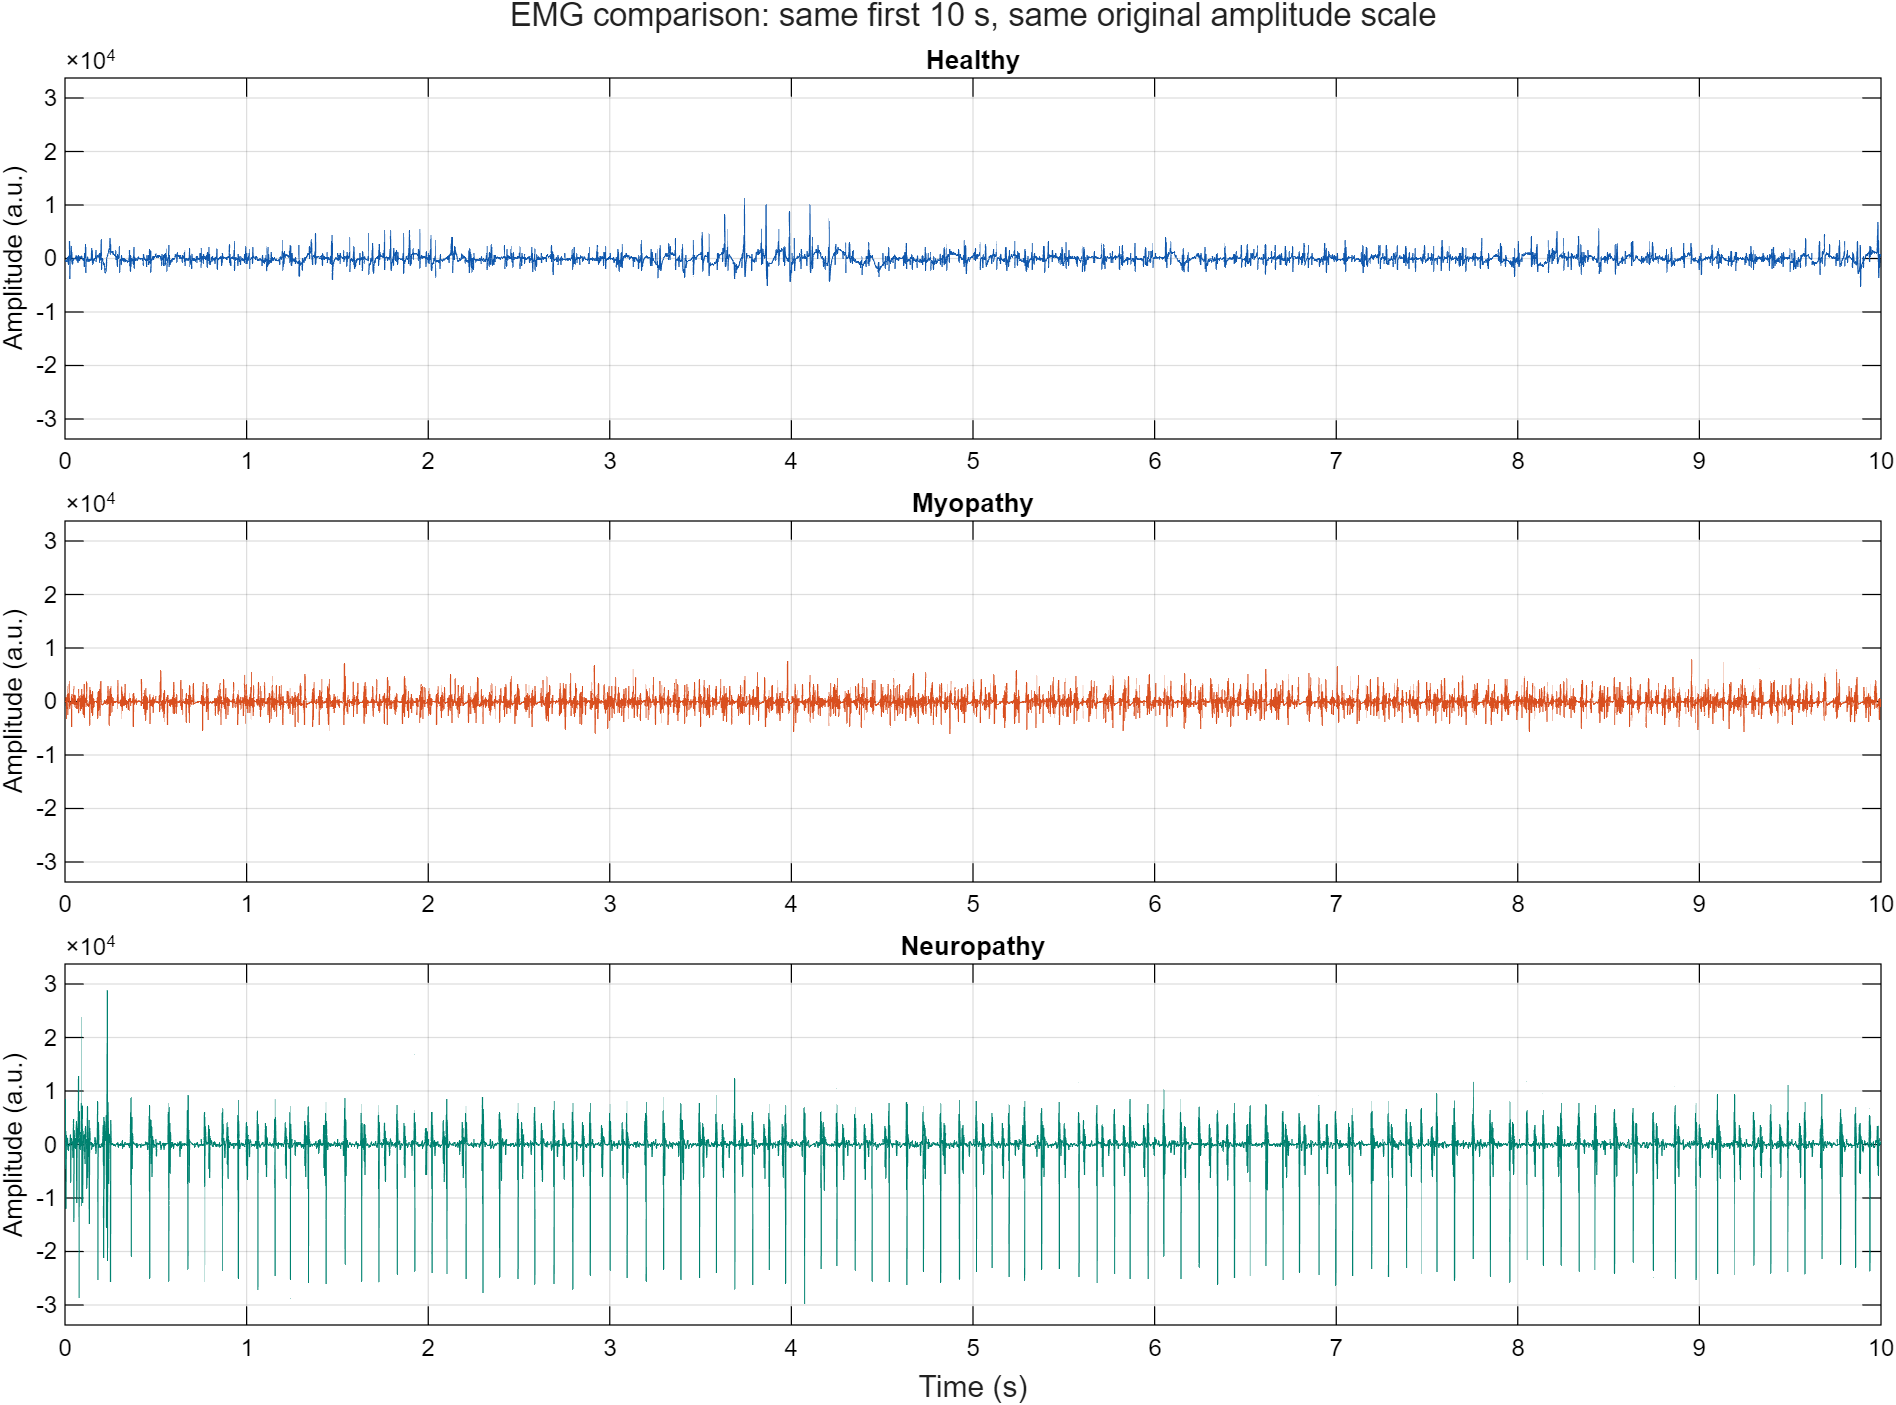
\includegraphics[width=0.95\textwidth]{fig26_emg_first_10s.png}
\caption{Comparison of the first ten seconds of all three recordings without amplitude normalization.}
\label{fig:emg10}
\end{figure}

To examine the local morphology, the intervals 1--1.2, 5--5.2 and 10--10.2~s were zoomed. Figure~\ref{fig:emgzoom} shows that the difference in amplitude and in the density of the transients cannot be determined from the whole recording alone; sharp potentials and local changes of shape are also important. In these samples, the large transients of neuropathy and the denser activity in parts of myopathy can be observed. Since the signal is the sum of several motor units, we do not attribute each peak to a single motor unit without separation.

\begin{figure}[H]
\centering
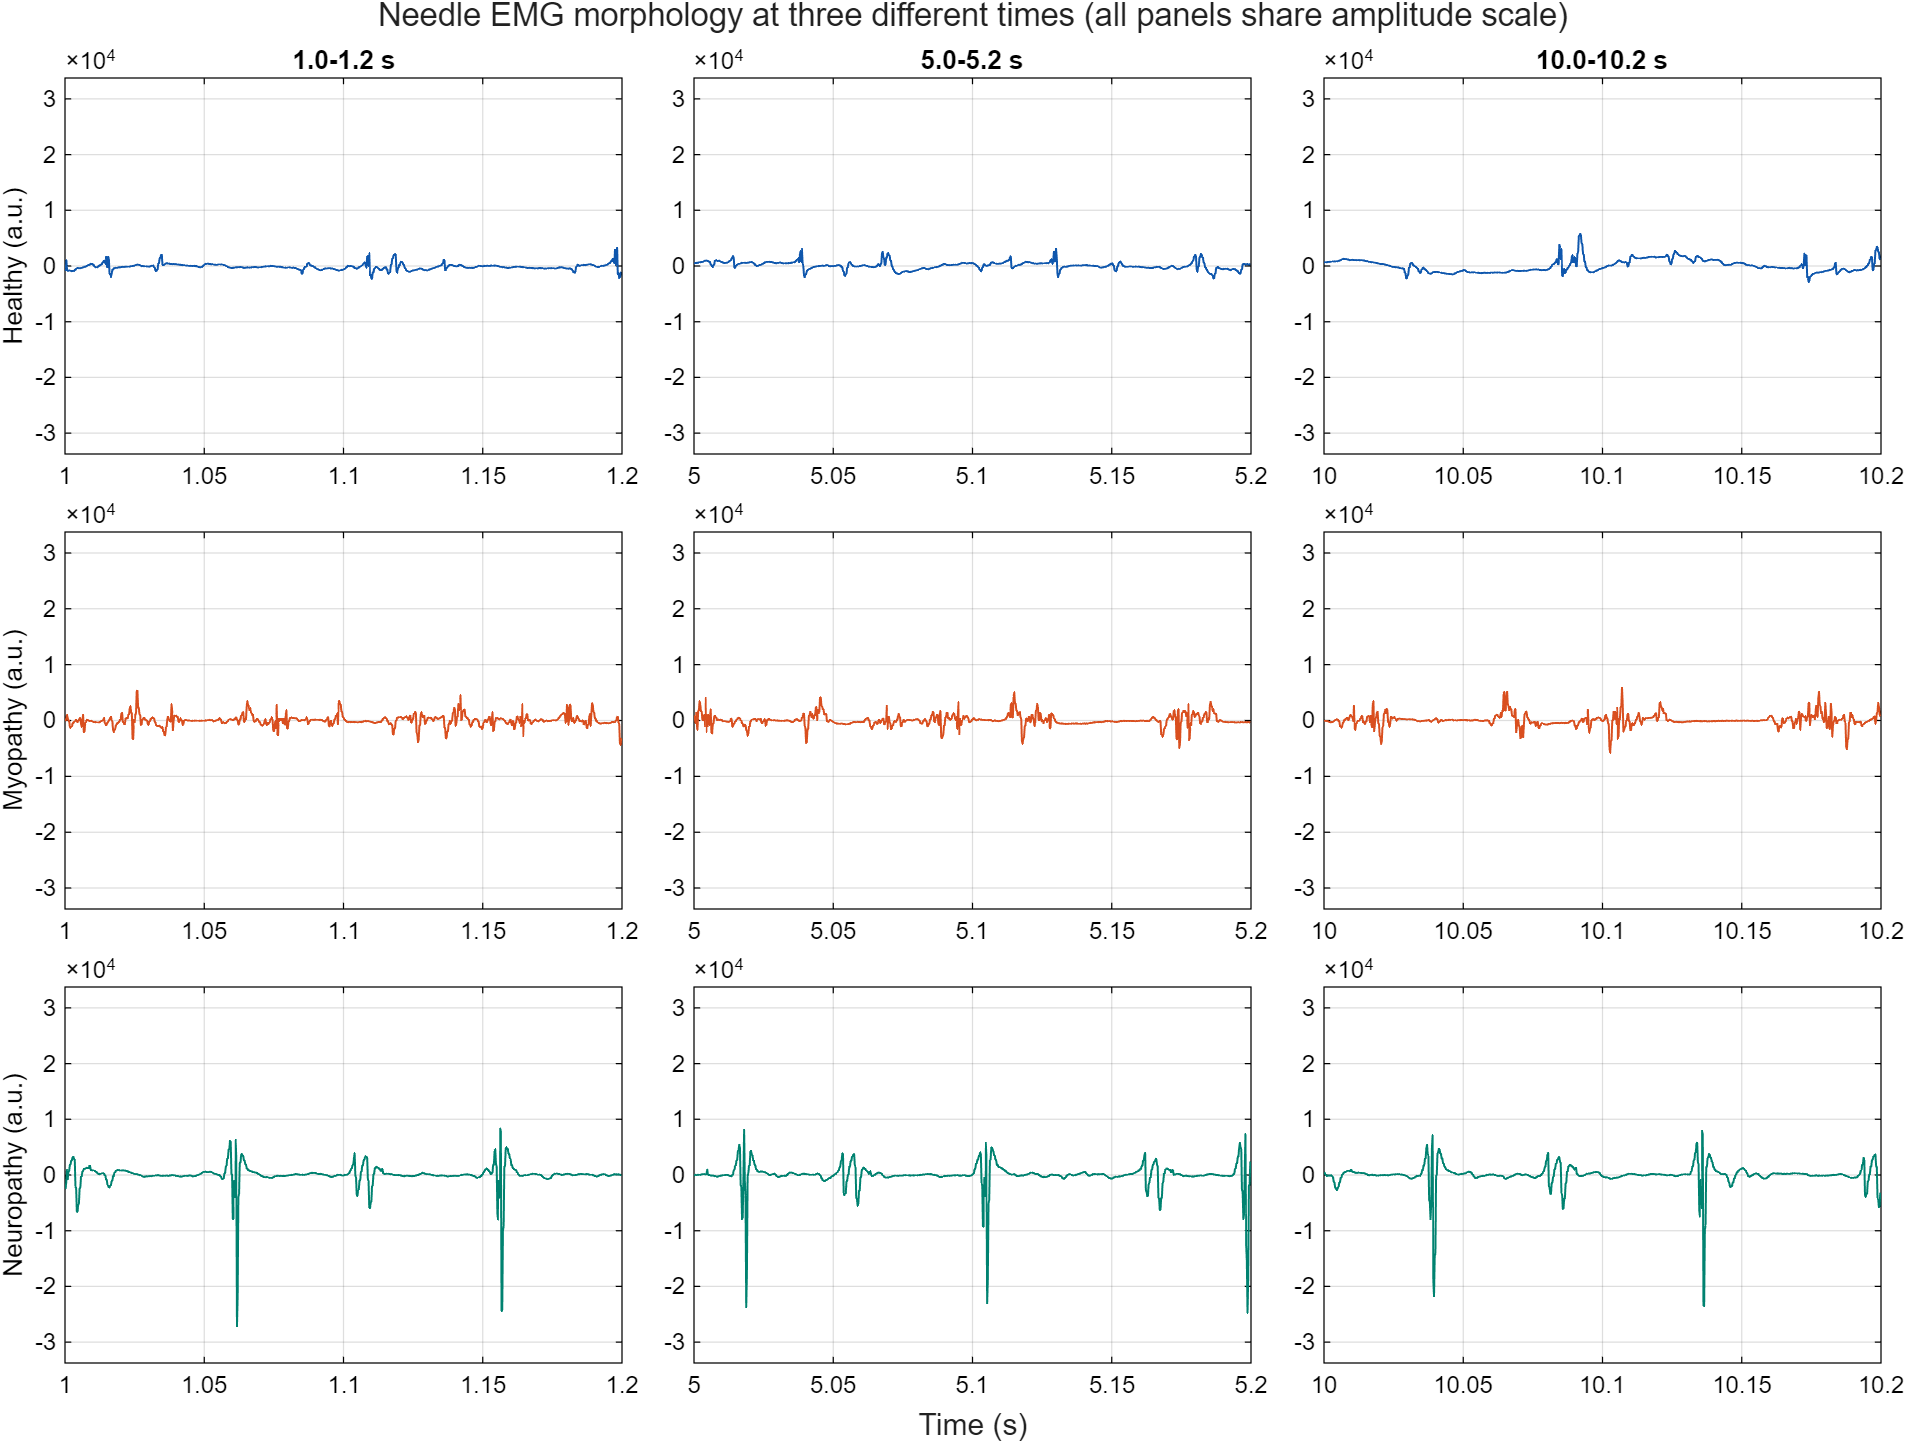
\includegraphics[width=0.95\textwidth]{fig27_emg_local_morphology.png}
\caption{Zoom on three short intervals of each subject, with a common amplitude axis.}
\label{fig:emgzoom}
\end{figure}

\subsection{Question 2: Frequency Spectrum and Spectrogram}
\begin{taskbox}
Plot the frequency spectrum and the time--frequency spectrum of the signal of each subject and compare them with each other.
\end{taskbox}

The Fourier transform and Welch's method were applied to the common ten-second interval after removing the mean. The spacing of the DFT is 0.1~Hz. Welch's estimate was computed with a Hann window of 1024 samples, i.e.\ 256~ms, an overlap of 512 and \texttt{nfft=4096}. Figure~\ref{fig:emgspec} shows both the absolute spectrum and the spectrum with unit area; the first compares the amplitude and power of the recordings, and the second separates the shape of the frequency distribution from the total power.

\begin{center}
\begin{tabular}{@{}lccc@{}}
\toprule
\textbf{Condition} & \textbf{AC RMS} & \textbf{Mean frequency (Hz)} & \textbf{Median frequency (Hz)}\\
\midrule
Healthy    &  820.08 & 166.49 &  63.31\\
Myopathy   &  962.72 & 429.21 & 238.52\\
Neuropathy & 2325.40 & 476.86 & 346.40\\
\bottomrule
\end{tabular}
\end{center}

The mean and the median frequency were computed from the power density:
\begin{equation}
\mathrm{MNF}=\frac{\int_{0}^{f_s/2} f\,P(f)\,df}{\int_{0}^{f_s/2}P(f)\,df},\qquad
\int_{0}^{\mathrm{MDF}}P(f)\,df=\frac12\int_{0}^{f_s/2}P(f)\,df .
\label{eq:mnf}
\end{equation}

\begin{figure}[H]
\centering
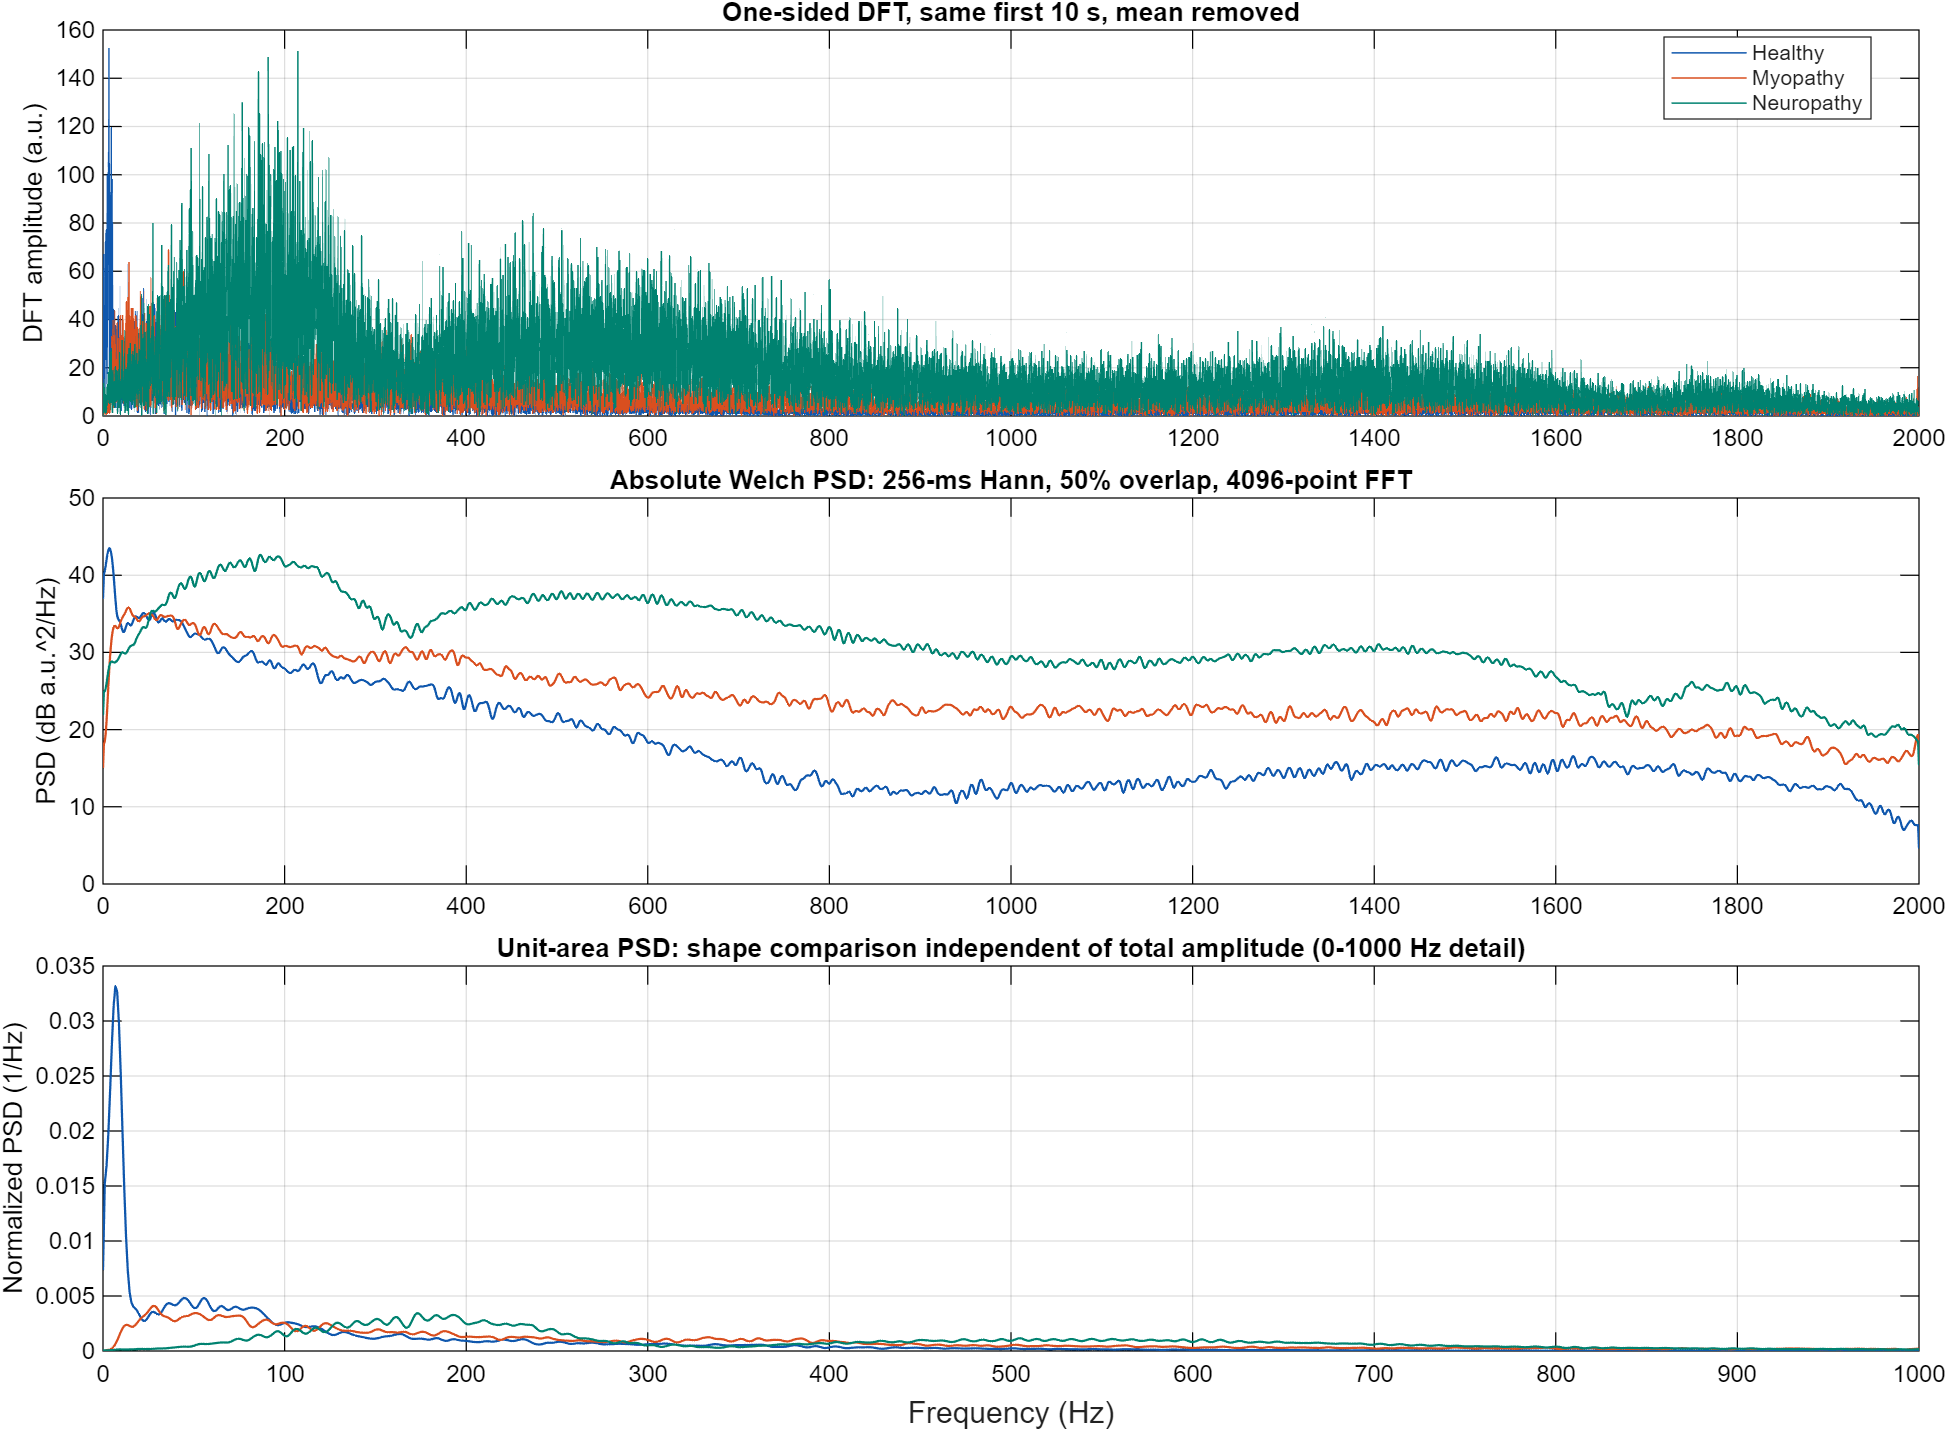
\includegraphics[width=0.95\textwidth]{fig28_emg_spectra.png}
\caption{Absolute amplitude spectrum and power density, and the unit-area power density, in the three muscle recordings.}
\label{fig:emgspec}
\end{figure}

In the present data, the RMS of myopathy is slightly greater than that of the healthy subject, and the RMS of neuropathy is much greater. This experiment is therefore not consistent with the claim that ``the total amplitude of myopathy is always smaller than that of a healthy subject.'' The mean and median frequencies of myopathy and neuropathy are also higher than those of the healthy sample. The Welch peak is about 6.84~Hz for the healthy subject, 28.32~Hz for myopathy and 172.85~Hz for neuropathy; the location of the peak is not the same as the center of mass of the spectrum or the firing rate of a single motor unit. Contraction, the location of the needle, the composition of the units and the quality of the recording also affect these indices.

In the complete neuropathy recording there are five samples with an absolute value of at least 32700, and its minimum is $-32767$. This closeness to the limit of a 16-bit integer raises the possibility of saturation, but by itself it is not proof of amplitude clipping. This issue can affect the amplitude and the fast content of the spectrum. The present analysis neither hid nor removed these samples.

In Figure~\ref{fig:emgstft}, a Hann window of 512 samples, i.e.\ 128~ms, an overlap of 448 samples and \texttt{nfft=2048} was used. The changes in energy intensity and the temporal transients show that the activity is not completely stationary. In neuropathy, more high-power, wide-frequency events are seen, and in the other two recordings the distribution of power over time has a different shape. The region after the end of the healthy or myopathy recording simply has no data. The Nyquist frequency of the present signal is 2000~Hz; the cutoff frequency of the analog filter of the original recording must not be taken as the Nyquist limit of the current version.

\begin{figure}[H]
\centering
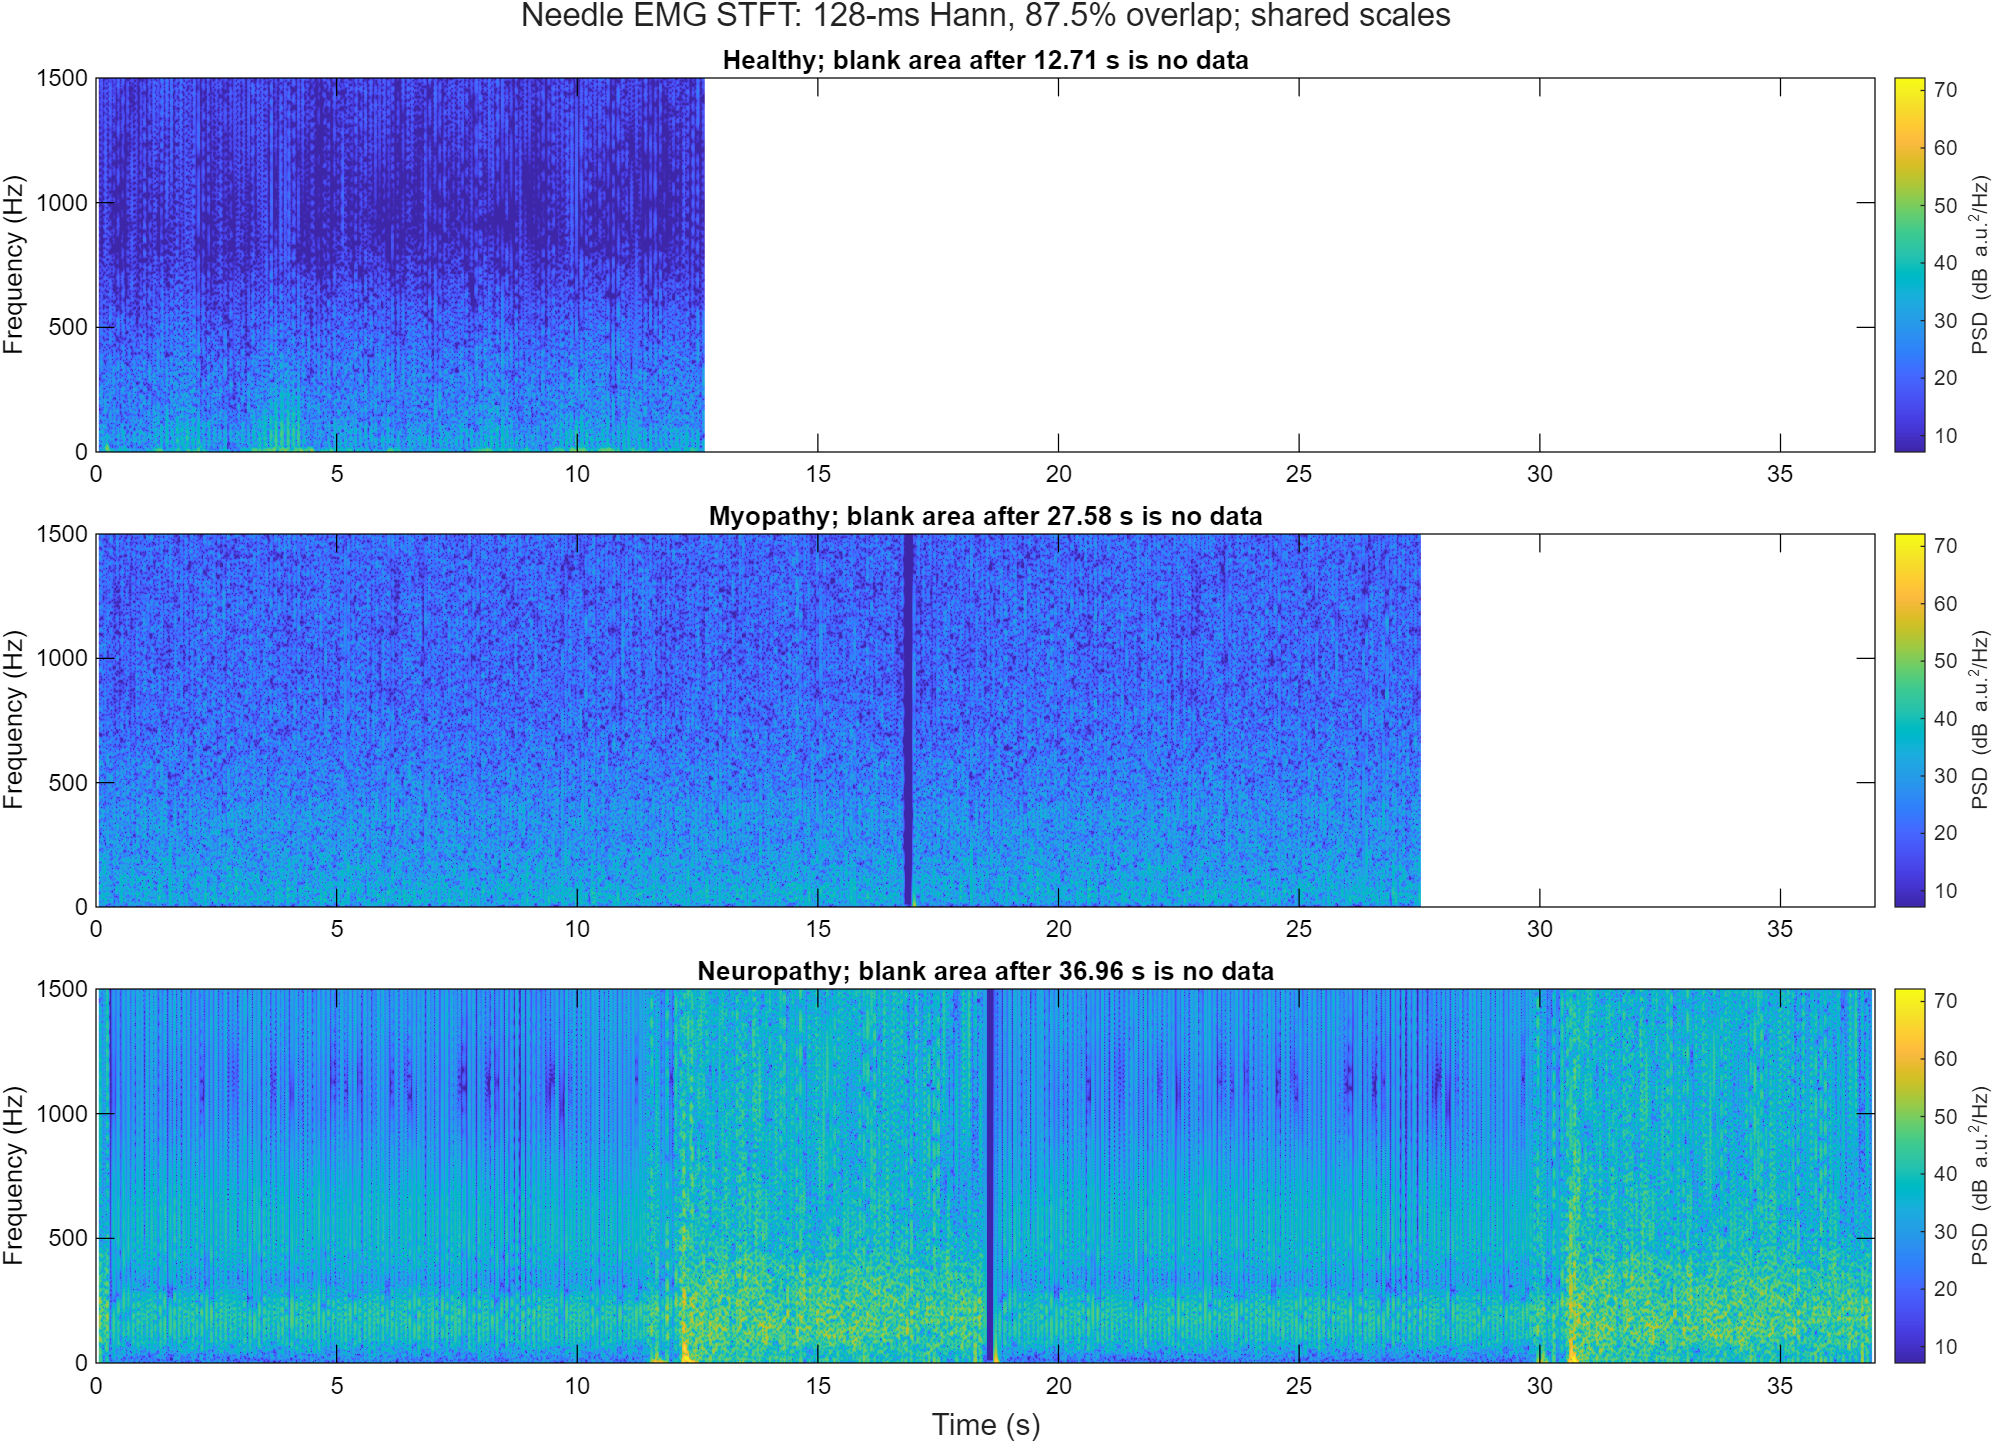
\includegraphics[width=0.95\textwidth]{fig29_emg_stft.png}
\caption{Spectrogram of the complete recordings of the three subjects with common time and frequency axes and common color limits.}
\label{fig:emgstft}
\end{figure}

\subsection{Question 3: Relating the Results to Neuropathy and Myopathy}
\begin{taskbox}
By studying the two diseases, Neuropathy and Myopathy, explain the results obtained in Questions 1 and 2.
\end{taskbox}

A motor unit consists of a motor neuron and the muscle fibers innervated by it, and the recorded signal is the sum of the potentials near the needle. In neuropathy, the main damage is in the nerve or the axon. In chronic neural damage, a reduction in the number of units and collateral reinnervation by the surviving axons can create larger units with longer, higher-amplitude potentials. This process is consistent with the larger transients in the present neuropathy recording, but to prove it, the potentials of the units must be analyzed individually.

In myopathy, the main damage is in the muscle itself. Damage to, or a reduction of, the active fibers of each unit can create shorter, smaller and shape-changed potentials. Nevertheless, the feature of the whole mixed signal is not the same as the characteristic of a single motor unit potential, and analyzing several potentials is important for drawing conclusions. In this experiment, separating the units and measuring the contraction force were not done; therefore the RMS or the median frequency of the three subjects is not a general diagnostic criterion for disease.

The larger transients in the neuropathy sample are consistent with changes in the motor units, but this cannot be proved from the spectrum alone. The myopathy data, in spite of an RMS slightly greater than that of the healthy subject, have a different shape and frequency distribution; this result shows that rules about the amplitude and duration of a single motor unit must not be generalized directly to the total power of the signal. The disease labels come from the data source and are not the product of a classifier built in this experiment.

\subsection{Core Implementation (EMG)}

\begin{lstlisting}[language=Matlab]
N = round(10*fs);                  % Equal duration for all three records
z = emg_healthym(1:N);
z = z(:)-mean(z);
[P,f] = pwelch(z,hann(1024,'periodic'),512,4096,fs);
normalizedPSD = P/trapz(f,P);      % Shape independent of total power
meanFrequency = trapz(f,f.*P)/trapz(f,P);
\end{lstlisting}

The motivation for choosing ten seconds and area normalization is to remove the differences in segment length from the comparison and to separate the difference in amplitude from the shape of the spectrum. This normalization does not remove the differences caused by the electrode location, the contraction intensity or artifacts. The features are stored in \texttt{results/emg\_features.csv}, and the complete code is in \texttt{code/lab1\_eog\_emg.m}.

\section{Conclusions and Reproducing the Experiment}

In the brain signal, the change in morphology was accompanied by a change in the spectral distribution, and the time--frequency analysis revealed the temporal location of these changes. Reducing the sampling rate after anti-aliasing filtering preserved the main band with a small difference and, at the same time, removed part of the fast power of the recording. In the cardiac signal, the two leads had common timing and different shapes, and separating the non-beat events from the real beats was essential for computing the intervals correctly. The eye data were mainly low-frequency and the muscle data contained faster transients; however, the physiological interpretation of both depended on the recording arrangement and on the limitations of the data.

All parts were run in MATLAB R2025b with the Signal Processing Toolbox. For reproduction, enter the folder of this report and run the command \texttt{run\_lab1}. The required data are in the \texttt{data} subfolder accompanying the package. By giving the path of the data to the function, using the original folder \texttt{Lab1\_data} is also possible. The code performs reading the data, checking the dimensions, computing the correct axes, building the plots and saving the tables. The output of a successful run is recorded in \texttt{results/run\_matlab.log}.

\begin{lstlisting}[language=Matlab]
results = run_lab1;
% Or:
results = run_lab1('C:\path\to\Lab 1_data');
\end{lstlisting}

The complete code is not repeated in the text of the report; only the decisive parts are given, with a statement of their purpose. The CSV and JSON files hold the exact numbers, the MAT files hold the results that can be loaded, and the PNG images hold the figures. The independent appendix of cardiac labels makes it possible to examine all the beats.

\end{document}
